\documentclass[11p,a4paper,fleqn]{report}

\usepackage{amsmath}		                          %Matheschreibweise...
\usepackage{amssymb}                              %...Und Symbole
%\usepackage{mathrsfs}
\usepackage[T1]{fontenc}
\usepackage[margin=2cm]{geometry}	                %Seitenrand
\usepackage{fancyhdr}	                            %Header
%\usepackage{graphicx}	                          %Bilder einfügen
%\usepackage{wrapfig}                              %Text um Graphiken "wickeln" (wrap)
\usepackage[most]{tcolorbox}
\usepackage{tikz,pgf,pgfplots}                    %Grafiken zeichnen
\usepackage{mdframed}	                            %Box			%\begin{mdframed} 		und			%\end{mdframed}
\usepackage{epstopdf}
\usepackage[utf8]{inputenc}
\usepackage[ngerman]{babel}
\usepackage{tabu}                                 %Bessere Tabellen
\usepackage{esvect}                               %Schönere Vektoren
\usepackage{listings}                             %Für Pseudocode/Code...
\usepackage{color}                                %...Und dessen Einfärbung
\usepackage{enumitem}                             %Angepasstes enumerieren
\usepackage{enumerate}                            %Zeichen der Enumerierung beliebig wählbar
\usepackage[hidelinks=true]{hyperref}
\usepackage[makeroom]{cancel}                     %Durchgestrichene Terme mit \cancel{}
\usepackage{tkz-tab}                              %Für Monotonietabellen??
\usepackage{marvosym}                             %Symbole wie Blitze und co. ...
\usepackage{stackengine}                          %Zeichen übereinander "stapeln"
\usepackage{epigraph}                             %Fürs Titelblatt
%\usepackage{array}			                          %Gleichungen mit mehr als einem Zeichen in der Zeile oder Tabellen
\usepackage{tocloft,titletoc,titlesec}            %Fürs Inhaltsverzeichnis

\pgfplotsset{compat=1.15}
\usetikzlibrary{arrows}
%\usetikzlibrary{fit}
%Für die Seitenangabe
\usepackage{flowfram}
\usepackage{nopageno}

\nonstopmode                                      %Fehler bei Kompilierung werden "leise" gestellt (sehr viel praktischer)



%Kapitel-Titelblatt
\makeatletter
\def\thickhrulefill{\leavevmode \leaders \hrule height 1.2ex \hfill \kern \z@}
\def\@makechapterhead#1{
  \vspace*{10\p@}%
  {\parindent \z@ \centering \reset@font
        \thickhrulefill\quad
        \huge\scshape\bfseries\textit{\@chapapp{}  \thechapter}\normalsize
        \quad \thickhrulefill
        \par\nobreak
        \vspace*{10\p@}%
        \interlinepenalty\@M
        \hrule
        \vspace*{10\p@}%
        \Huge \bfseries #1 \par\nobreak
        \par
        \vspace*{10\p@}%
        \hrule
        \vskip 50\p@
  }}


%Beweis:
\newenvironment{Beweis}
  {\begin{tcolorbox}[colback=gray!5!white,colframe=gray!75!black,opacityframe=0.5, opacitybacktitle=0.5,sharpish corners,boxrule=0pt,frame hidden,title=Beweis,breakable,break at=23cm,pad at break=1mm,]}
  {\end{tcolorbox}}


%Definition:
\newenvironment{Definition}
  {\begin{tcolorbox}[colback=red!7!white,colframe=red!70!black,sharpish corners,boxrule=0pt,frame hidden,title=Definition \thesubsection]}
  {\end{tcolorbox}}


%Theorem:
\newenvironment{Theorem}
  {\begin{tcolorbox}[colback=blue!5!white,colframe=blue!75!black,sharpish corners,boxrule=0pt,frame hidden,title=Theorem]}
  {\end{tcolorbox}}

%Beispiel
\newenvironment{Beispiel}
  {\par\noindent\normalfont\par\nopagebreak%
  \begin{mdframed}[
     linewidth=2pt,
     linecolor=green,
     bottomline=false,topline=false,rightline=false,
     innerrightmargin=0pt,innertopmargin=0pt,innerbottommargin=0pt,
     innerleftmargin=1em,% Distanz zwischen vertikaler Strich & Inhalt
     skipabove=.5\baselineskip
   ]\underline{Beispiel:}\\}
{\end{mdframed}}


%Bemerkung
\newenvironment{Bemerkung}
  {\par\noindent\normalfont\par\nopagebreak%
  \begin{mdframed}[
     linewidth=2pt,
     linecolor=yellow,
     bottomline=false,topline=false,rightline=false,
     innerrightmargin=0pt,innertopmargin=0pt,innerbottommargin=0pt,
     innerleftmargin=1em,% Distanz zwischen vertikaler Strich & Inhalt
     skipabove=.5\baselineskip
   ]\underline{Bemerkung:}\\}
{\end{mdframed}}


%GTR-Tipp
\newenvironment{GTR-Tipp}
  {\par\noindent\normalfont\par\nopagebreak%
  \begin{mdframed}[
     linewidth=2pt,
     linecolor=gray,
     bottomline=false,topline=false,rightline=false,
     innerrightmargin=0pt,innertopmargin=0pt,innerbottommargin=0pt,
     innerleftmargin=1em,% Distanz zwischen vertikaler Strich & Inhalt
     skipabove=.5\baselineskip
   ]\underline{GTR-Tipp:}\\}
{\end{mdframed}}


%Codebox, aufrufbar mit \begin{lstlisting}[typ_der_Sprache]
\definecolor{dkgreen}{rgb}{0,0.6,0}
\definecolor{gray}{rgb}{0.5,0.5,0.5}
\definecolor{mauve}{rgb}{0.58,0,0.82}
\lstset{
  backgroundcolor = \color{lightgray},
  frame=tb,
  aboveskip=3mm,
  belowskip=3mm,
  showstringspaces=false,
  columns=flexible,
  basicstyle={\small\ttfamily},
  numbers=false,
  numberstyle=\tiny\color{gray},
  keywordstyle=\color{blue},
  commentstyle=\color{dkgreen},
  stringstyle=\color{mauve},
  breaklines=true,
  breakatwhitespace=true,
  tabsize=3
}


\usepackage[scale=.9]{tgheros} % or helvet
\renewcommand{\familydefault}{\sfdefault}

\begin{document}
  \begin{titlepage}
	\begin{center}
	\line(1,0){300}  \\
	[0,5cm]
	\Huge{\bfseries Schülerskript SMP} \\
	[3cm]
	\textsc{ \bfseries MATHEMATIK}  \\
	[15cm]
	\small{\today} \\
	[2cm]
	\tiny{Clara, Bruno, Pascal, Rémy, ..., 1$^{ere}$ SMP}
	\end{center}
\end{titlepage}

  \blankpage
  \tableofcontents
  \begin{dynamiccontents*}{frameD-1a}
\begin{tikzpicture}
\draw(0,0) node [fill=titlepagecolor, minimum width=1cm, minimum height=1cm]{
{\sffamily\bfseries\large\color{white}\thepage}
};
\end{tikzpicture}
\end{dynamiccontents*}

\begin{dynamiccontents*}{frameD-1b}
\begin{tikzpicture}
\draw(0,0) node [fill=titlepagecolor, minimum width=1cm, minimum height=1cm]{
{\sffamily\bfseries\large\color{white}\thepage}
};
\end{tikzpicture}
\end{dynamiccontents*}

  %%%%%%%%%%%%%%%%%%%%%%%%%%%%%%%%%%%%%%%%%%%%%%%%%%%%%%%%%%%%%%%%%%%%%%%%%%%%%%
  %Kapitel bitte hier einbinden:
  \chapter{Folgen}



\begin{Definition}
Eine Funktion , bei der nur natürlichen Zahlen eine reelle Zahl zugeordnet wird, nennt man Folge.\\
Folgen können auch nur für Teilbereiche von $\N$ definiert sein.\\
$(a_{n})_{n\in\N}$ bezeichnet die Folge, wobei $a:\N\rightarrow\R$
\end{Definition}

\begin{Bemerkung}
In einem Ausdruck muss das $n$ immer dasselbe bleiben!
\end{Bemerkung}
		\section{Verschiedene Darstellungen}


	\subsection{Explizite Darstellung}

\begin{Definition}
Wenn ein beliebiges Glied der Folge direkt berechenbar ist, ist ihre Darstellung explizit.
\end{Definition}

\begin{Beispiel}
\begin{enumerate}
\item  $a_{n}=3^n \Rightarrow a_{4}=3^4=91$
\item Die Folge der $n-ten$ positiven, ungeraden Zahl:\\
$a_{n}=1+2\cdot(n-1) \Rightarrow$ Die 8. positive, ungerade Zahl ist $ a_{8}=1+2\cdot(8-1)=15$
\end{enumerate}
\end{Beispiel}


	\subsection{Rekursive Darstellung}

\begin{Definition}
Wenn für die Berechnung des $n-ten$ Gliedes einer Folge das $(n-1)-te$ Glied benötigt wird, ist ihre Darstellung rekursiv.
In diesen Fällen braucht man immer ein Startglied, oft $a_{0}$ oder $ a_{1}$.
\end{Definition}

\begin{Beispiel}
\begin{enumerate}
\item  $a_{n}=3\cdot a_{n-1}+2;a_{0}=5$\\
\indent$a_{1}=3\cdot a_{1-1}+2=3\cdot a_{0}+2=3\cdot5+2=17$\\
\indent$a_{2}=3\cdot a_{2-1}+2=3\cdot a_{1}+2=3\cdot17+2=53$\\
\indent$a_{3}=3\cdot a_{3-1}+2=3\cdot a_{2}+2=3\cdot53+2=159$\\
\indent und so weiter...
\item Die Folge der $n-ten$ positiven, ungeraden Zahl:\\
$a_{n}=a_{n-1}+2;a_{1}=1$
\end{enumerate}
\end{Beispiel}

\begin{Bemerkung}
Für manche Folgen sind beide Darstellungen möglich, wobei die explizite Darstellung oftmals viel praktischer ist, da die Berechnung der Folgeglieder anhand der rekursiven Darstellung schnell sehr aufwendig wird.
\end{Bemerkung}

\begin{GTR-Tipp}
Wie man im GTR macht
\end{GTR-Tipp}

\subsubsection{Web-Diagramme}
Hier handelt es sich um eine graphisches Verfahren, das dazu dient, das Verhalten einer Folge, deren Darstellung rekursiv ist, zu untersuchen.\\
Dazu muss man der rekursiven Folgenvorschrift eine Funktion $f(a_{n-1})=a_{n}$ zuordnen, sodass - grob gesagt - " die Funktion das Gleiche mit x macht, dass die Folge macht, um von $a_{n}$ auf $a_{n+1}$ zu kommen. Zusätzlich zeichnet man in ein kartesisches Koordinatensystem die Hauptdiagonale ein (entspricht dem Graphen von $f(x)=x$).\\
Dann trägt man das erste Folgeglied auf die Abzissenachse ein und verbindet ihn mit der entsprechenden Funktion anhand eines vertikalen\\

\begin{Bemerkung}
Dieses Verfahren kann aber ausschließlich bei rekusiven Folgen angewendet werden, bei denen keine zusätzliche Abhängigkeit von $n$ vorliegt (Beispiel: $a_{n}=3\cdot a_{n-1}+3+4\cdot n$) oder die Rekursivitätsebene den 1. Grad überschreitet, was bedeutet, dass $a_{n}$ nicht nur in Abhängigkeit von $a_{n-1}$ beschrieben wird, sondern zusätzlich von mindestens $a_{n-2}$ (Beispiel: die Fibonacci-Folge).\\
\end{Bemerkung}

\begin{GTR-Tipp}
Verwendung mit dem GTR
\end{GTR-Tipp}


		\section{Auffällige Folgen}


	\subsection{Arithmetische Folgen}

\begin{Definition}
Eine Folge wird arithmetisch genannt, wenn die Differenz zweier aufeinander folgender Glieder konstant ist.
\begin{enumerate}
\item Rekursive Darstellung:\\
\indent $a_{n}=a_{n-1}+d$
\item Explizite Darstellung:\\
\indent Mit Startglied $a_{0}$: $a_{n}=a_{0}+n\cdot d$\\
\indent Mit Startglied $a_{1}$: $a_{n}=a_{1}+(n-1)\cdot d$\\
\indent Mit Startglied $a_{x}$: $a_{n}=a_{x}+(n-x)\cdot d$
\end{enumerate}
\end{Definition}

\begin{Bemerkung}
Letzteres gilt auch für beliebige Folgeglieder, also ist $a_{n}=a_{p}+(n-p)\cdot d;n,p\in\N$
\end{Bemerkung}

\begin{Beispiel}
$a_{n}=a_{n-1}+3;a_{0}=0\Leftrightarrow a_{n}=0+n\cdot3$
\end{Beispiel}

\begin{Bemerkung}
Jedes Folgeglied einer solchen Folge ist das arithmetische Mittel seines Vorgängers und Nachgängers: $a_{n}=\dfrac{a_{n-1}+a_{n+1}}{2}$
\end{Bemerkung}

	\subsection{Geometrische Folgen}

\begin{Definition}
Eine Folge wird geometrisch genannt, wenn der Quotient zweier aufeinander folgender Glieder konstant ist.
\begin{enumerate}
\item Rekursive Darstellung:\\
\indent $a_{n}=a_{n-1}\cdot q$
\item Explizite Darstellung:\\
\indent Mit Startglied $a_{0}$: $a_{n}=a_{0}\cdot q^n$\\
\indent Mit Startglied $a_{1}$: $a_{n}=a_{1}\cdot q^{n-1}$\\
\indent Mit Startglied $a_{x}$: $a_{n}=a_{x}\cdot q^{n-x}$\\
\end{enumerate}
\end{Definition}

\begin{Bemerkung}
Letzteres gilt auch für beliebige Folgeglieder, also ist $a_{n}=a_{p}\cdot q^{n-p};n,p\in\N$
\end{Bemerkung}

\begin{Beispiel}
$a_{n}=a_{n-1}\cdot3;a_{0}=2\Leftrightarrow a_{n}=2\cdot3^n$
\end{Beispiel}

\begin{Bemerkung}
Jedes Folgeglied einer solchen Folge ist das geometrische Mittel seines Vorgängers und Nachgängers:\\
 $a_{n}=\sqrt{a_{n-1}\cdot a_{n+1}}$
\end{Bemerkung}

		\section{Klassifizierung von Folgen}


	\subsection{Monotonie}

\begin{Definition}
Eine Folge $(a_n)_n\in\N$ heißt monoton \begin{cases} \text{\textcolor{red}{steigend/wachsend}}\\\text{\textcolor{orange}{fallend/abnehmend}}\end{cases} wenn \begin{cases} \textcolor{red}{a_n+1\geq a_n}\\\textcolor{orange}{a_n+1\leq a_n}\end{cases}.\\\\
Gelten dabei sagar \textbf{strikte} Ordnungsrelationen ($>$ oder $<$), dann ist $(a_n)$ \textbf{streng} monoton wachsend beziehungsweise abnehmend.

\end{Definition}

	\subsection{Beschränktheit}

\begin{Definition}
Man nennt eine  Folge $(a_n)n\in\N$ nach  \begin{cases} \text{\textcolor{red}{oben}}\\\text{\textcolor{orange}{unten}}\end{cases} \textbf{beschränkt}\\ wenn es eine Zahl  \begin{cases} \textcolor{red}{S\in\R}\\\textcolor{orange}{s\in\R}\end{cases} gibt mit  \begin{cases} \textcolor{red}{a_n\leq S}\\\textcolor{orange}{a_n\geq s}\end{cases} $\forall n\in\N$.\\\\
\textcolor{red}{$S$} ist eine \textcolor{red}{obere }Schranke\\
\textcolor{orange}{$s$} ist eine \textcolor{orange}{untere} Schranke
\end{Definition}

\begin{Definition}
Die kleinste obere Schranke ist das \textbf{Supremum} der Menge $\{a_n;n\in\N\}$.\\
Die größte untere Schranke ist das \textbf{Infimum} der Menge $\{a_n;n\in\N\}$.
\end{Definition}


\begin{Definition}
Eine nach \textbf{oben und unten} beschränkte Folge heißt \textbf{beschränkte} Folge (suite bornée).}
\end{Definition}

\begin{Beispiel}
\end{Beispiel}



	\subsection{Konvergenz}

\begin{Definition}
Eine Folge $(a_n)n\in\N$ heißt konvergent, wenn sie einen Grenzwert besitzt.\\
Man sagt $a_n$ konvergiert gegen $g=\lim\limits_{n\to\infty}a_n$.
\end{Definition}



\begin{Theorem}
Eine Folge $(a_n)n\in\N$ konvergiert gegen $g$ genau dann, wenn $(a_n-g)$ gegen den Wert $0$ konvergiert:\\
$$\lim\limits_{n\to\infty}a_n=g\Leftrightarrow \lim\limits_{n\to\infty}(a_n-g)=0$$
\end{Theorem}

\begin{Theorem}
Eine monotone Folge ist genau dann konvergent, wenn sie beschränkt ist.
\end{Theorem}

\begin{Beweis}
\end{Beweis}

\subsubsection{Divergenz}
\begin{Definition}
Eine Folge $(a_n)n\in\N$, die keinen Grenzwert $g\in\R$ besitzt (nicht kovergiert), wird \textbf{divergent} genannt.
\end{Definition}

\subsubsection{Epsilon-n0-Definition}
\begin{Definition}
$$(a_n) \text{ konvergiert gegen $g$} \Leftrightarrow \forall  \epsilon > 0 \exists n_0 \in\N \forall n\geq n_0 |a_n-g|<\epsilon$$
\end{Definition}
\subsubsection{Grenzwertsätze}


Die Grenzwertsätze führen die Grenzwerte komplizierter Folgen auf einfachere Grenzwertbetrachtungen bekannter Folgen zurück.\\
\begin{Theorem}
\end{Theorem}



  \chapter{Reihen}

\begin{Definition}
Eine Reihe ist eine Folge, deren Glieder die Partialsummen einer anderen Folge ist. Das bedeutet, dass das $n-te$ Glied der Reihe, die Summe der ersten $n$ Glieder einer anderen Folge ist. \\
Man hat also:

\begin{enumerate} 
\item Mit Startglied $a_{0}$: $s_{n}=\sum\limits_{i=0}^{n-1}a_{i}$
\item Mit Startglied $a_{1}$: $s_{n}=\sum\limits_{i=1}^{n}a_{i}$
\item Mit Startglied $a_{x}$: $s_{n}=\sum\limits_{i=x}^{n+x-1}a_{i}$
\end{enumerate}

\end{Definition}

\begin{Bemerkung}
In manchen Fällen steht $s_{n}$ für die Partialsumme einer anderen Folge bis zum $n-ten$ Glied.
Dann gilt für ein beliebiges Startglied $a_{x}$ der Folge: $s_{n}=\sum\limits_{i=x}^{n}a_{i}$
\end{Bemerkung}

		\section{Artithmetische Reihen}


  \documentclass[../MAIN/main.tex]{subfiles}
\begin{document}
\chapter{Funktionsuntersuchung}\label{Funktionsuntersuchung}
\chapterauthor{Bruno}

Die \textbf{Analysis} (griechisch  análysis, deutsch "`Aufl"osung"') ist ein Teilgebiet der Mathematik. Die Untersuchung von reellen und komplexen Funktionen hinsichtlich Stetigkeit, Differenzierbarkeit und Integrierbarkeit z"ahlt zu den Hauptgegenst"anden der Analysis. Die hierzu entwickelten Methoden sind in allen Natur- und Ingenieurwissenschaften von großer Bedeutung.

\section{Stetigkeit}

\begin{Definition}
Eine Funktion ist stetig an der Stelle $x_{0}$, wenn:
\begin{enumerate}
\item $x_{0}\in D$
\item $\lim\limits_{x \rightarrow x_{0}} {f(x)}$ existiert
\item $\lim\limits_{x \rightarrow x_{0}^{\pm}} {f(x)}=f(x_{0})$\\
\end{enumerate}
\end{Definition}\\

Stetigkeit ist eine lokale Eigenschaft. Die Funktion $f$ hei"st dann stetig, wenn sie an jeder Stelle ihrer Definitionsmenge stetig ist.

\begin{Bemerkung}
\begin{Theorem}
	Ist $f$ stetig und $I\subset \R$ ein reelles Intevall, dann ist $f(I)$ ebenfalls ein Intervall. Ist $f$ zudem streng monoton, so ist die Umkehrfunktion $f^{-1}$ ebenfalls stetig.
\end{Theorem}
\end{Bemerkung}

\begin{Bemerkung}
Stetige Funktionen haben sehr angenehme Eigenschaften, die intuitiv mit der ''Definition'' des Stiftes, welcher beim Zeichnen des Funktionsgraphen nicht angehoben wird, im Zusammenhang stehen.\\
\\
So sagt der \textbf{Zwischenwertsatz} aus, dass eine reelle, im Intervall $[a;b]$ stetige Funktion $f$ jeden Wert zwischen $f(a)$ und $f(b)$ ainnimmt.\\
Haben $a$ und $b$ zudem verschiedene Vorzeichen, so verspricht der Zwischenwertsatz mindestens eine Nullstelle von $f$ in diesem abgeschlossenen Intervall. Dieser Sonderfall ist als \textbf{Nullstellensatz} von Bolzano bekannt.
\end{Bemerkung}

\begin{Theorem}[- Zwischenwertsatz]
Ist $f:[a;b]\Rightarrow$ eine stetige reelle Funktion die auf einem Intervall definiert ist, dann existiert zu \textbf{jedem} $s \in [f(a);f(b)]$ bzw. $[f(b);f(a)]$ (vom Vorzeichen der Funktionswerte abh"angig) \textbf{ein} $c \in [a;b] $ mit $f(c)=s$
\end{Theorem}

\subsubsection{Stetige Fortsetzungen}

Beim Vereinfachen von gebrochenrationalen Funktionen ist Vorsicht geboten, denn eine hebbare Definitionsl"ucke ''aufzuheben'' ver"andert den Definitionsbereich der Funktion. Die daraus resultierende Funktion wird \textbf{stetige Fortsetzung} genannt.



\section{Differenzierbarkeit}

\begin{Definition}
Eine Funktion ist differenzierbar an der Stelle $x_{0} \in D$, wenn der beitseitige Grenzwert des Differenzenquotienten f"ur $h\rightarrow 0$ existiert. Anschaulich soll Die Funktion links und rechts des $x_{0}$ die selbe Ableitung haben. \\
\\
$\lim\limits_{h \rightarrow 0^{+}} {\dfrac{f(x_{0}+h)-f(x_{0})}{h}} = \lim\limits_{h \rightarrow 0^{-}} {\dfrac{f(x_{0}+h)-f(x_{0})}{h}} =f'(x_{0})$\\
\\
Dieser Grenzwert ist die \textbf{Ableitung} von $f$ an der Stelle $x_{0}$.\\
Die Funktion hei"st differenzierbar, wenn sie $\forall x \in D$ differenzierbar ist.\\
\end{Definition}
\\

Die Funktion $f(x)=|x|$ ist nicht differenzierbar, da bei der Stelle $x_{0}=0$ der linksseitige Grenzwert des Differenzenquotienten ($\lim\limits_{h \rightarrow 0^{-}}{f'(x_{0})=-1}$) nicht mit dem rechtsseitigen Grenzwert (1) "ubereinstimmt.\\

\subsection{Zusammenhang zwischen Stetigkeit und Differenzierbarkeit}

Ist eine Funktion $f$ an der Stelle $x_{0}$ differenzierbar, so ist sie an dieser Stelle auch stetig.
Die Umkehrung gilt erst einmal nicht, aber es gibt eine verneinende Aussage: Ist $f$ an der Stelle $x_{0}$ nicht stetig, so ist sie hier auch nicht differenzierbar.\\
\begin{Theorem}
	$f$ differenzierbar $\Rightarrow f$ stetig.
\end{Theorem}
\begin{Bemerkung}
	Ist eine Funktion differenzierbar und ist ihre Ableitung zus"atzlich stetig, dann wird sie \textbf{Stetig differenzierbar} genannt.
\end{Bemerkung}

\section{Ableitungsregeln}


Ein Ableitungswert gibt die Steigung an einem bestimmten Punkt an. Im Allgemeinen und zum Beweisen wird der Differentenquotient ben"otigt, um eine Ableitungsfunktion zu definieren, es geht aber in vielen F"allen schneller.

\begin{Theorem}[- Produktregel]
Sind die Funktionen $u$ und $v$ an der Stelle $x_{0}$ $\in$ $D$ differenzierbar, dann ist die Funktion $f(x)=u(x)\cdot v(x)$ bei $x_{0}$ auch differenzierbar und es gilt: \\
$$f'(x_{0}) = u'(x_{0})v(x_{0})+u(x_{0})v'(x_{0})$$
\end{Theorem}
\begin{Beweis}
$
\begin{array}{rcl}
\lim\limits_{h \rightarrow 0} {\dfrac{f(x_{0}+h)-f(x_{0})}{h}} & = & \lim\limits_{h \rightarrow 0} {\dfrac{u(x_{0})v({x_{0}+h)-u(x_{0})v(x_{0})}}{h}}\\
&=&\lim\limits_{h \rightarrow 0} {\dfrac{u(x_{0}+h)v(x_{0}+h)\textcolor{red}{-u(x_{0})v(x_{0}+h)+u(x_{0})v(x_{0}+h)}-u(x_{0})v(x_{0}) }{h}}\\
&=&\lim\limits_{h \rightarrow 0} {\dfrac{u(x_{0}+h)v(x_{0}+h)-u(x_{0})v(x_{0}+h)}{h}} + \lim\limits_{h \rightarrow 0} {\dfrac{u(x_{0})v(x_{0}+h)-u(x_{0})v(x_{0})}{h}}\\
&=&\lim\limits_{h \rightarrow 0} {v(x_{0}+h)\dfrac{u(x_{0}+h)-u(x_{0})}{h}} \lim\limits_{h \rightarrow 0} {u(x_{0})\dfrac{v(x_{0}+h)-v(x_{0})}{h}}\\
&=& v(x_{0})\lim\limits_{h \rightarrow 0}{\dfrac{u(x_{0}+h)-u(x_{0})}{h}} +u(x_{0}) \lim\limits_{h \rightarrow 0} {\dfrac{v(x_{0}+h)-v(x_{0})}{h}}\\
&=& u'(x_{0})v(x_{0}) - u(x_{0})v'(x_{0})
\end{array}
$
\end{Beweis}

\begin{Theorem}[- Quotientenregel]
Sind die Funktionen $u$ und $v$ an der Stelle $x_{0}$ $\in$ $D$ differenzierbar, dann ist die Funktion $f(x)=\frac{u(x)} {v(x)}$ bei $x_{0}$ auch differenzierbar und es gilt: \\
$$f'(x_{0})=\frac{u'(x_{0})\cdot v(x_{0})-u(x_{0})\cdot v'(x_{0})}{v^2(x_{0})}$$\\
\end{Theorem}
\begin{Beweis}
$
\begin{array}{rcl}
\lim\limits_{h \rightarrow 0} {\dfrac{f(x_{0}+h)-f(x_{0})}{h}}&=& \lim\limits_{h \rightarrow 0} { \dfrac{ \dfrac{u(x_{0}+h)} {v(x_{0}+h)}- \dfrac{u(x_{0})}  {v(x_{0})}}  {h}}\\
&=&\lim\limits_{h \rightarrow 0} {\dfrac{\dfrac {u(x_{0}+h)}{v(x_{0}+h)}-\dfrac {u(x_{0})} {v(x_{0})}}   {h}}\\
&=&\lim\limits_{h \rightarrow 0} {\dfrac {\dfrac{  u(x_{0}+h)v(x_{0})}{v(x_{0}+h)v(x_{0})}   -\dfrac{u(x_{0})v(x_{0}+h)}{v(x_{0})v(x_{0}+h))}} {h}}\\
&=&\lim\limits_{h \rightarrow 0} {\dfrac     {u(x_{0}+h)v(x_{0})-u(x_{0})v(x_{0}+h)}    {v(x_{0}+h)v(x_{0})h }}\\
&=&\lim\limits_{h \rightarrow 0} {\dfrac {u(x_{0}+h)v(x_{0}) \textcolor{red}{-u(x_{0})v(x_{0})} -u(x_{0})v(x_{0}+h) \textcolor{red}{+u(x_{0})v(x_{0})}}  {v(x_{0}+h)v(x_{0})h}   }\\
&=&\lim\limits_{h \rightarrow 0} {\dfrac   {\dfrac{u(x_{0}+h)v(x_{0})-u(x_{0})v(x_{0})}{h}  -   \dfrac{u(x_{0})v(x_{0}+h)-u(x_{0})v(x_{0})} {h} }    {v(x_{0}+h)v(x_{0})}}\\
&=&\lim\limits_{h \rightarrow 0} { \dfrac     {\dfrac{u(x_{0}+h)-u(x_{0})}{h} v(x_{0})  -   u(x_{0}) \dfrac   {v(x_{0}+h)-v(x_{0})}  {h}  }         {v(x_{0}+h)v(x_{0})}     }\\
&=&\lim\limits_{h \rightarrow 0} { \dfrac  {\lim\limits_{h \rightarrow 0} {\dfrac{u(x_{0}+h)-u(x_{0})}{h}   }v(x_{0})  - u(x_{0}) \lim\limits_{h \rightarrow 0} { \dfrac{ v(x_{0}+h)-v(x_{0})}{h}   }  }      {v(x_{0})v(x_{0})}}    \\
&=& { \dfrac{u'(x_{0})v(x_{0})-u(x_{0})v'(x_{0})} {(v(x_{0}))^2}    }\\
\end{array}
$
\end{Beweis}

\begin{Theorem}[- Kettenregel]
Die Funktion $v$ sei an der Stelle $x_{0}$ differenzierbar und die Funktion $u$ an der Stelle $v(x_{0})$. Dann ist die Funktion $f=u\circ v$ mit der Gleichung $f(x)= u(v(x))$ an der Stelle $x_{0}$ differenzierbar. Es gilt:\\

$$f'(x_{0})=v'(x_{0})\cdot u'(v(x_{0}))$$
\end{Theorem}

\subsection{Tangente und Normale}
\begin{Theorem}
Ist die Funktion $f$ differenzierbar an der Stelle $x_{0}$, dann hat die \textbf{Tangente} an dem Graphen von $f$ die Steigung $a=f'(x_{0})$ und den Y-Achsenabschnitt $b=-f'(x_{0})\cdot x_{0}+f(x_{0})$. Daraus ergibt sich die Tangentengleichung:\\

$$T_{x_{0}}(x)=f'(x_{0})\cdot (x-x_{0})+f(x_{0}) $$ \\
\end{Theorem}
\\
\begin{Bemerkung}
	Eine Merkhilfe dazu ist das Wort "`Fuxufu"', wobei "`u"' dem $x_{0}$ entspricht.\\
\end{Bemerkung}
\\
\begin{Definition}
Die \textbf{Normale} an der Stelle $x_{0}$ bezeichnet die Gerade, die genau senkrecht zur Tangente steht und diese im Ber"uhrpunkt des Graphen schneidet.\\
$$N_{x_{0}}(x)=-\frac{1}{f'(x_{0})}\cdot (x-x_{0})+f(x_{0})$$\\
\end{Definition}

\section{Vollst"andige Funktionsuntersuchung}


\subsection{Definitionsbereich}

Am Anfang muss der Definitionsbereich angegeben werden, um eventuelle Divisionen durch null zu vermeiden. Man achte dabei auch auf hebbare Definitionsl"ucken (siehe ''Stetigkeit'') \\


\subsection{Achsenschnittpunkte}

Es gibt zwei Arten von Achsenschnittpunkten:
\begin{enumerate}
\item X-Achsenschittpunkte (Nullstellen), die man mit der notwendigen und hinreichenden Bedingung f"ur Nullstellen $f(x)=0$ herausfindet
\item Y-Achsenschnittpunkt, den man durch einsetzen bekommt: $f(0)$ \\
\end{enumerate}

\subsection{Symmetrie}

\subsubsection{Y-Achsensymmetrie}

Durch L"osung der Gleichung $f(x)=f(-x)$ findet man heraus ob die Funktion achsensymmetrisch ist.\\
Zudem ist die Funktion dann achsensymmetrisch, wenn nur gerade Exponenten vorhanden sind.\\
Die Funktion nennt man \textbf{gerade}.\\

\subsubsection{Symmetrie zum Origo}

Durch L"osung der Gleichung $f(x)=-f(-x)$ findet man heraus ob die Funktion punktsymmetrisch ist.\\
Zudem ist die Funktion dann punktsymmetrisch, wenn nur ungerade Exponenten vorhanden sind.\\
Die Funktion nennt man \textbf{ungerade}.\\


\subsubsection{Symmetrie zu einem beliebigen Punkt}
\begin{Definition}
Symmetrie zu einem Punkt liegt vor, wenn f"ur den Punkt $P(x_{0}|y_{0})$ gilt:\\
$$f(x_{0}+h)-y_{0}=-f(x_{0}-h)+y_{0}$$
\end{Definition}
\begin{Beispiel}
\\
$f(x)=\frac{x}{x-1}$\\
\\
Aus dem Schnittpunkt der Asymptoten kann man vermuten, dass $f(x)$ achsensymmetrisch zum Punkt $P(1|1)$ ist.\\
\\
$\left. \begin{array}{rcl}
\Rightarrow f(x_{0}+h)-y_{0}=\frac{1+h}{1+h-1}-1=\frac{1}{h}\\
\\
\Rightarrow -f(x_{0}-h)+y_{0}=-[\frac{1-h}{1-h-1}+1]=\frac{1}{h}\\
\end{array}\right\} \frac{1}{h}=\frac{1}{h}$ Die Funktion $f$ ist zu $P$ symmetrisch.\\
\end{Beispiel}


\subsection{Grenzwerte}

\begin{Definition}
Das Symbol $\lim\limits_{x \rightarrow x_{0}}f(x)$ mit $x_{0} \in \overline{\R}$ ($\pm \infty$ eingeschlossen) bezeichnet den Limes der reellen Funktion $f:D\rightarrow \R$ f"ur den Grenz"ubergang von $x$ gegen eine Stelle $x_{0}$, wobei $x_{0}$ nicht umbedingt in der Definitionsmenge von $f$ enthalten sein muss.\\
\\
Eine Zahl $g \in \overline{\R}$ ist der Grenzwert einer Funktion $f:D\rightarrow \R$ f"ur $x\rightarrow x_{0}$, falls f"ur jede Folge $(a_{n})_{n\in \N}$ mit Folgegliedern aus $D$ und Grenzwert $x_{0}$ die Folge $(f(a_{n}))_{n\in \N}$ den Grenzwert $g$ hat.
\begin{center}
$\lim\limits_{x \rightarrow x_{0}}f(x) = g $\quad $\Leftrightarrow$ \quad $\forall (a_{n})_{n\in \N}$ mit $\lim\limits_{n \rightarrow \infty}a_{n}=x_{0} : \lim\limits_{n \rightarrow \infty}f(a_{n})=g$
\end{center}
\end{Definition}

\begin{Definition}
	Regel von l'Hospital: für Grenzwerte des Typs $0/0$ und $\infty/\infty$\\
	Seien zwei differenzierbare Funktionen $f$ und $g$ und gelte entweder\\
	$$\lim\limits_{x \rightarrow x_{0}}g(x) = \lim\limits_{x \rightarrow x_{0}}f(x) = \infty \qquad \text{ODER} \qquad  \lim\limits_{x \rightarrow x_{0}}g(x) = \lim\limits_{x \rightarrow x_{0}}f(x) = 0$$\\
	(sie sind also entweder konvergent gegen $0$ oder bestimmt divergent) dann gilt:\\
	$$\lim\limits_{x \rightarrow x_{0}} \dfrac{f(x)}{g(x)} = \lim\limits_{x \rightarrow x_{0}}\dfrac{f'(x)}{g'(x)}$$
\end{Definition}

\begin{Bemerkung}
	\begin{enumerate}
		\item Falls die Funktionsvorschrift nicht direkt ein Bruch ist (siehe 2. Beispiel) sollte man diese erst zu einem Bruch umformen, um mit der Hospital-Regel fortfahren zu können.
		\item ACHTUNG: Die Hospital-Regel ist nicht umkehrbar!
	\end{enumerate}
\end{Bemerkung}

\begin{Beispiel}

$f(x) = \dfrac{\sin(x)}{x} \qquad x_{0} = 0\qquad \qquad D=\R\backslash\{0\}$ \\\\
$\Rightarrow \lim\limits_{x \rightarrow x_{0}}f(x) = \lim\limits_{x \rightarrow x_{0}}\dfrac{\sin(x)}{x} = \lim\limits_{x \rightarrow x_{0}} \dfrac{\cos(x)}{1} = 1 $\\\\ \\

$g(x) = x\cdot \log\left(\dfrac{x+1}{x-1}\right) \qquad $f"ur $ x\to \infty \qquad \qquad D=\R\backslash\{1\}$ \\\\
\begin{array}{rcl}
$\Rightarrow \lim\limits_{x \rightarrow \infty} g(x) & = & \lim\limits_{x \rightarrow \infty} x\cdot \log\left(\dfrac{x+1}{x-1}\right) $\\
&=& \lim\limits_{x \rightarrow \infty} \dfrac{\log\left(\dfrac{x+1}{x-1}\right)}{\dfrac{1}{x}}\\
&=& \lim\limits_{x \rightarrow \infty} \dfrac{\dfrac{x-1}{x+1} \cdot \dfrac{-2}{(x-1)^2}}{-\dfrac{1}{x^2}}\\
&=& \lim\limits_{x \rightarrow \infty} \dfrac{\dfrac{-2}{x^2-1}}{-\dfrac{1}{x^2}}\\
&=& \lim\limits_{x \rightarrow \infty} \dfrac{2x^2}{x^2-1} = 2 \\
\end{array}

\end{Beispiel}


\subsection{Asymptoten}

Eine Asymptote ist eine Gerade oder Kurve, die sich dem Graphen einer Funktion immer weiter ann"ahert. Dabei unterscheidet man verschiedene F"alle:\\
\begin{Definition}
\begin{enumerate}
	\item \textbf{Senkrechte Asymptote:}\\
	Hat $f$ an der stelle $x_{0}$ eine Polstelle, und gilt:
		$$\lim\limits_{x \rightarrow x_{0^{\pm}}} f(x) = \pm \infty$$
	dann ist die Gerade $x=x_{0}$ eine senkrechte Asymptote von $f$.

	\item \textbf{Waagerechte Asymptote:}\\
	Konvergiert $f$ f"ur $x\rightarrow \infty$ gegen eine reelle Zahl $g\in \R$, das heißt $\lim\limits_{x \rightarrow \infty }{f(x)}=g$, dann ist die Gerade $y=g$ die \textbf{waagerechte} Asymptote von $f$. Das Gleiche gilt f"ur $\lim\limits_{x \rightarrow -\infty}$.\\
	Bei gebrochenrationalen Funktionen ist dies der Fall, wenn der Z"ahlergrad kleiner (dann ist $g=0$) oder gleich dem Nennergrad $m$ ist.

	\item \textbf{Schr"age Asymptote:}\\
	Sie ist eine Gerade ($g:\R \rightarrow \R$), der sich $f$ mit $|x|\rightarrow \infty$ beliebig ann"ahert:
	$$\lim\limits_{x \rightarrow \infty}{[f(x)-g(x)]}=0 \text{ oder } \lim\limits_{x \rightarrow -\infty}{[f(x)-g(x)]}=0$$
	Bei einer gebrochenrationalen Funktion ist der ''Fehlergrad'', das hei"st der Abstand von $g$ zu $f$ durch den Rest der Polynomdivision von Z"ahler mit Nenner gegeben.

	\item \textbf{Asymptotische Kurven:}\\
	Indem man in der Definition der schr"agen Asymptote auch Polynome zul"asst, erh"alt man N"aherungskuven, die die gleiche Limesbedingung erf"ullen m"ussen:
	$$\lim\limits_{x \rightarrow \infty}{[f(x)-P(x)]}=0 \text{ oder } \lim\limits_{x \rightarrow -\infty}{[f(x)-P(x)]}=0$$
	Diese erscheinen bei gebrochenrationalen Funktion mit $n>m+1$.
\end{enumerate}
\end{Definition}

\subsection{Monotonie}

\begin{Definition}
Eine stetige Funktion $f$ mit $a,b\in I \subset D_{f}$ ist:\\
\begin{enumerate}
\item ... auf dem Intervall $I$ monoton wachsend, wenn $\forall a < b: f(a)\leq f(b)$
\item ... auf dem Intervall $I$ monoton fallend, wenn $\forall a < b: f(a) \geq f(b)$ \\
\end{enumerate}
Wenn die Ordnungsrelation strikt sind, dann wird die Funktion als \textbf{streng monoton} bezeichnet.\\
Die Funktion $f$ hat eine Ableitungsfunktion $f'$. Falls $f$...
\begin{enumerate}
\item monoton wachsend auf $I$ ist, dann ist $f'(x)\geq0$, \quad $\forall x \in I$
\item monoton fallend auf $I$ ist, dann ist $f'(x)\leq0$, \quad $\forall x \in I$
\item konstant auf $I$ ist, dann ist $f'(x)=0$, \quad $\forall x \in I$
\end{enumerate}
Beim Aufstellen der Monotonietabelle sind Definitionsl"ucken zu beachten.\\
\\
Es handelt sich dabei um eine Tabelle, die die Definitionsmenge in Intervalle mit monotonen Steigungsverhalten unterteilt wird. Das Monotonieverhalten ver"andert sich an Extrem- oder Polstellen.\\
\end{Definition}
\begin{Bemerkung}
$f$ sei eine Funktion...
\begin{description}
\item[$\bullet$] dann ist die Zahl $S$ obere Schranke, wenn $\forall x : f(x)\leq S$. $f$ hei"st in diesem Fall nach oben beschr"ankt. Die in diesem Fall kleinstm"ogliche Zahl wird \textbf{Supremum} genannt: sup$f$
\item[$\bullet$] dann ist die Zahl $s$ untere Schranke, wenn $\forall x : f(x) \geq s$. $f$ ist in diesem Fall nach unten beschr"ankt. Die in diesem Fall gr"o"stm"ogliche Zahl wird \textbf{Infimum} genannt: inf$f$
\end{description}
\end{Bemerkung}
\begin{Bemerkung}
Eine Funktion $f$ ist...
\begin{description}
\item[$\bullet$] \textbf{konvergent}, wenn sie einen Grenzwert $g\in\R$ hat
\item[$\bullet$] \textbf{bestimmt divergent}, wenn sie  \textbf{keinen} reellen Grenzwert, also $\lim\limits_{x \rightarrow +\infty}{f(x)} = \pm \infty$
\item[$\bullet$] \textbf{unbestimmt divergent}, wenn es keine Zahl $g\in\overline{\R}$ ($\overline{\R} = \R$ mit $\infty$ und $-\infty$) gibt mit $\lim\limits_{x \rightarrow +\infty}{f(x)} = g$
\end{description}
\end{Bemerkung}
\begin{Beispiel}
	$f(x)=x\cdot\sin{x}$
\end{Beispiel}

\subsection{Extremstellen}

F"ur die Bestimmung von Extremstellen gilt es zwei Bedingungen zu "uberpr"ufen:\\

Hat an einer Stelle $x_{0}$ die erste Ableitung von $f$ eine Nullstelle, also $f'(x_{0}) = 0$, dann handelt es sich um eine Extremstelle \textbf{oder} um einen Sattelpunkt. Diese Bedingung ist die notwendige Bedingung f"ur eine Extremstelle. Mit ihr ist eine grobe Kategorisierung gemacht, eine Extremstelle ist noch nicht bewiesen.  \\\\

Hat $f'$ an der Stelle $x_{0}$ einen Vorzeichenwechsel oder ist $f''(x_{0})\neq 0$, dann ist der Sonderfall des Wendepunktes ausgeschlossen und es handelt sich um deine Extremstelle. Es gilt also: \\\\ $\exists! $ $ x_{0} \in I \subseteq D_{f} : f(x_{0}) \geq oder \leq f(x) $ \\\\ Der Punkt $P(x_{0}|f(x_{0}))$ hei"st Hochpunkt oder Tiefpunkt. Diese Bedingung ist die hinreichende Bedingung f"ur eine Extremstelle.

\subsection{Wendestellen}

F"ur die Bestimmung von Wendestellen gilt es auch zwei Bedingungen zu "uberpr"ufen:\\

Hat an einer Stelle $x_{0}$ die zweite Ableitung von $f$ eine Nullstelle, also $f''(x_{0}) = 0$, dann handelt es sich um eine Wendestelle \textbf{oder} um einen geraden Abschnitt. Diese Bedingung ist die notwendige Bedingung f"ur eine Wendestelle. \\\\

Hat $f''$ an der Stelle $x_{0}$ einen Vorzeichenwechsel oder ist $f'''(x_{0})\neq 0$, dann ist der Sonderfall ausgeschlossen und es handelt sich um deine Wendestelle. Der Punkt $W(x_{0}|f(x_{0}))$ hei"st Wendepunkt. Diese Bedingung ist die hinreichende Bedingung f"ur eine Wendestelle.\\\\

\begin{Bemerkung}
  \label{NEW-Regel}
Eine Hilfsformel, die den Zusammenhang zwischen den verschiedenen Ableitungen einfach darstellt ist die NEW-Regel:\\\\

\begin{minipage}[b]{0.2\linewidth}
\\
N $=$ Nullstellen\\
E $=$ Extremstellen\\
W $=$ Wendestellen
\end{minipage}
\hfill \vline \hfill
\begin{minipage}[b]{0.4\linewidth}
\begin{array}{rcccccl}
f & \qquad \qquad& N & E & W & & \\
f' & \qquad \qquad && N & E & W & \\
f'' & \qquad \qquad &&& N & E & W \\
\end{array}
\end{minipage}
\end{Bemerkung}

\subsection{Funktionseinordnung}

\begin{Definition}
Jede Funktion $f$ bildet auf verschiedene Weise eine Definitionsmenge $D_{f}$ auf eine Wertmenge $W_{f}$ ab. \\Hat eine Menge $G$ eine größere Mächtigkeit (notiert $|G|$) als $K$, dann besitzt $G$ mehr Elemente als $K$. Dies gilt eigentlich nicht für überabzählbar unendlich große Mengen, diese sind theoretisch alle gleich groß (unendlich groß!).\\\\
Eine Funktion $f$ ist ...
\begin{description}
\item[$\bullet$] \textbf{surjektiv}, wenn sie jedes Element der Zielmenge mindestens einmal als Funktionswert annimmt. Das heißt, jedes Element der Zielmenge hat mindestens ein Urbild.\\\\
$$\forall y \in W_{f} \quad \exists x \in D_{f}:\quad f(x)=y $$\\\\
$|D_{f}| \geq |W_{f}|$. \quad Beispiel: $\qquad f(x)=\sin{x} $\\

\item[$\bullet$] \textbf{injektiv}, wenn zu jedem Element der Wertmenge höchstens ein (oder auch gar kein) Element der Definitionsmenge existiert. Zwei verschiedene Elemente $x_{1}$ und $x_{2}$ der Definitionsmenge bilden also nie auf den gleichen Term $y$ der Wertmenge ab.\\\\
$$\forall x_{1}, x_{2} \in D_{f} :\qquad f(x_{1}) = f(x_{2}) \quad \Rightarrow \quad x_{1}=x_{2} $$\\\\
\danger \quad Dies bedeutet \textbf{nicht}:\quad $\forall x_{1}, x_{2} \in D_{f} :\qquad x_{1} = x_{2} \quad\Rightarrow\quad f(x_{1}) = f(x_{2}) $ \\\\
$|D_{f}| \leq |W_{f}|$.\quad Beispiel: $\quad f(x)=2x$ \quad mit \quad $D_{f}=\Z$\\

\item[$\bullet$] \textbf{bijektiv}, wenn eine vollständige Paarbildung existiert. Jedes Element der Wertmenge besitzt genau ein Element der Definitionsmenge und jedes Element der Definitionsmenge besitzt genau ein Element der Wertmenge. Eine Funktion ist genau dann bijektiv, wenn sie sowohl surjektiv, als auch injektiv ist.\\\

$|D_{f}| = |W_{f}|$. \quad Beispiel: $\qquad f(x)=x^3 $\\\\
\end{description}
\end{Definition}
\begin{Bemerkung}
Ausführlichere Erklärungen hier, einfach auf die Links klicken:\\
\href{http://www.math.uni-konstanz.de/~huynh/Vorkurs2015/Vorlesung_12.pdf}{\textcolor{blue}{Uni Vorlesungsskript}} \qquad oder \qquad
\href{https://www.mathe-online.at/mathint/fun1/i_isb.html}{\textcolor{blue}{Überschaubar(er) mit Graphen}} \\
\end{Bemerkung}


\subsection{Umkehrbarkeit}


\\
\\
\begin{Definition}
Sei $f$ eine Funktion mit $f:D_{f}\mapsto W_{f}$ mit $x\mapsto y$, dann ist die Funktion genau dann eindeutig umkehrbar, wenn es zu jedem $y \in W_{f}$ \textbf{genau ein} $x \in D_{f}$ existiert. \\ \\
Wenn diese Funktion umkehrbar ist, dann existiert auch eine Umkehrfunktion $\overline{f}(x)$ die jedem $x \in W_{f}$ genau ein $y\in D_{f}$ zuordnet, analog zur Funktion, nur andersrum, also mit $y\mapsto x$\\
\\Es gilt: \qquad $D_{\overline{f}} = W_{f}}$ \qquad und \qquad $W_{\overline{f}}=D_{f}$
\end{Definition}

\begin{Bemerkung}
Es gibt viele Funktionen (surjektive Funktionen) die nicht in ihrer vollst"andigen Definitionsmenge umkehrbar sind, zum Beispiel $x^n$ mit $n$ als gerade Zahl, $\sin(x), \tan(x)$, und viele mehr.  Hier beschr"ankt man die Funktion auf ein bestimmtes Intervall, um sie umkehren zu k"onnen.\\ \\
Die Funktion $f(x)=x^2$ mit $D_{f}=\R$ und $W_{f}=\R_{0}^{+}$ hat f"ur $y=4$ zwei Urbilder: $-2$ und $2$. Beschr"ankt man die Funktion auf $D_{f}=\R_{0}^{+}$, ist sie umkehrbar und die Umkehrfunktion lautet $\overline{f}(x)=\sqrt{x}$\\
\end{Bemerkung}\\ \\ \\

\begin{Definition}
Umkehrregel oder Inversenregel\\

Sei $f$ eine bijektive (also umkehrbare), differenzierbare, reelle Funktion bei der gilt: $f'(x)\neq 0$, dann ist die Umkehrfunktion auch differenzierbar mit der Ableitung \\\\
$\overline{f}'(y) = \dfrac{1}{f'(\overline{f}(y))} = \dfrac{1}{f'(x)}$

\end{Definition}

\begin{Beweis}
\begin{array}{rcccl}
$\Rightarrow & \overline{f}(f(x)) &=& x $&\qquad \qquad | $ ableiten \\\\
$\Leftrightarrow & \overline{f}'(f(x)) \cdot f'(x) &=& 1 &$ \\\\
$\Leftrightarrow & \overline{f}'(f(x)) &=& \dfrac{1}{f'(x)}&$\\\\
$\Leftrightarrow & \overline{f}'(y) &=& \dfrac{1}{f'(x)}$& \qquad \qquad | $ mit $y=f(x)$  \\
\end{array}
\end{Beweis}


\begin{minipage}[b]{0.5\linewidth}
\begin{Bemerkung}
Anschaulich ist eine Umkehrfunktion eine Axenspiegelung entlang der Winkelhalbierende am Ursprung, also dem Funktionsgraphen von $f(x)=x$
\end{Bemerkung}
\begin{Beispiel}
Die Funktion $f(x)=x^2$ mit $D_{f} = \R_{0}^{+}$ ist umzukehren. Leichtes Spiel...\\ \\
\begin{array}{rcccccl}
$\Rightarrow $& $y$ &$ = $&$ x^2$\\
$\Leftrightarrow $&$ x $&$ = $&$ \pm \sqrt{y}$ &\quad \small { \textit{Variablen tauschen}}\\
$\Leftrightarrow $&$ y $&$ = $&$ \pm \sqrt{x}$\\
$\Rightarrow $&$ \overline{f}(x)$&$=$&$ \pm \sqrt{x}$\\

\end{array}
\end{Beispiel}

\end{minipage}
\hfill
\begin{minipage}[b]{0.4\linewidth}
\definecolor{ffvvqq}{rgb}{1.,0.3333333333333333,0.}
\definecolor{qqttcc}{rgb}{0.,0.2,0.8}
\definecolor{ttqqqq}{rgb}{0.2,0.,0.}
\definecolor{cqcqcq}{rgb}{0.7529411764705882,0.7529411764705882,0.7529411764705882}
\begin{tikzpicture}[line cap=round,line join=round,>=triangle 45,x=0.7cm,y=0.7cm]
\draw [color=cqcqcq,, xstep=1.4cm,ystep=1.4cm] (-3.,-3.8) grid (7.8,5.8);
\draw[->,color=black] (-3.,0.) -- (7.8,0.);
\foreach \x in {-2.,2.,4.,6.}
\draw[shift={(\x,0)},color=black] (0pt,2pt) -- (0pt,-2pt) node[below] {\footnotesize $\x$};
\draw[->,color=black] (0.,-3.8) -- (0.,5.8);
\foreach \y in {-2.,2.,4.}
\draw[shift={(0,\y)},color=black] (2pt,0pt) -- (-2pt,0pt) node[left] {\footnotesize $\y$};
\draw[color=black] (0pt,-10pt) node[right] {\footnotesize $0$};
\clip(-3.,-3.8) rectangle (7.8,5.8);
\draw[line width=0.4pt,color=ttqqqq,smooth,samples=100,domain=-3.0:7.8] plot(\x,{(\x)});
\draw[line width=2.pt,color=qqttcc,smooth,samples=100,domain=-3.0:7.8] plot(\x,{(\x)^(2.0)});
\draw[line width=1.2pt,color=ffvvqq,smooth,samples=100,domain=2.4000001559384112E-8:7.8] plot(\x,{sqrt((\x))});
\draw[line width=1.2pt,dash pattern=on 3pt off 3pt,color=ffvvqq,smooth,samples=100,domain=2.4000001559384112E-8:7.8] plot(\x,{0-sqrt((\x))});
\draw (2.4867074111243883,-0.32603907695652323) node[anchor=north west] {$p \left(x \right) \, = \,-\sqrt{x}$};
\draw (2.8429337294434633,1.8367635699807134) node[anchor=north west] {$h \left(x \right) \, = \,\sqrt{x}$};
\draw (-2.958466311752897,1.0734214592969828) node[anchor=north west] {$g \left(x \right) \, = \,x^{2}$};
\begin{scriptsize}
\draw[color=ttqqqq] (-5.4774952770092105,-5.504043061094496) node {$f$};
\draw[color=qqttcc] (-1.635339986567762,4.164957007566092) node {$g$};
\draw[color=ffvvqq] (1.6215863523494927,1.0352543537627963) node {$h$};
\draw[color=ffvvqq] (1.5706968783039106,-0.669543026764202) node {$p$};
\end{scriptsize}
\end{tikzpicture}
\end{minipage}\\\\



\subsection{Beispiel}

$f(x) = \dfrac{4x^2 -8x +4}{2x-1} = \dfrac{(2x-2)^2}{2x-1}$ \qquad \qquad $D_{f}=\R \backslash \{ \frac{1}{2} \}$ \\ \\ \\
$f'(x) = \dfrac{(8x-8)(2x-1)-(4x^2-8x+4)(2)}{(2x-1)^2} = \dfrac{16x^2-8x-16x+8-8x^2+16x-8}{4x^2-4x+1} = \dfrac{8x^2-8x}{(2x-1)^2}$\\ \\ \\
\begin{array}{rcccl}
$f''(x) $ &$ = $&$ \dfrac{\textcolor{red}{(16x-8)}(4x^2-4x+1)-(8x^2-8x)\textcolor{red}{(8x-4)}}{(\textcolor{red}{(2x-1)}^2)^2}$\\ \\
& $=$ & $\dfrac{\cancel{(2x-1)}\cdot 8 \cdot (4x^2-4x+1) - (8x^2-8x)\cdot 4 \cdot \cancel{(2x-1)}}{(2x-1)^{\cancel{4} 3}}$ & $=$ & $\dfrac{8}{8x^3-12x^3+6x-1} $\\
\end{array}

\subsubsection{Achsenschnittpunkte}

\underline{Bestimmung der Nullstelle(n):} \\

\begin{array}{rcccl}
$\Rightarrow    &    f(x)    &    =    &    0 & D=\R \backslash \{ \frac{1}{2} \}$ \\
$\Leftrightarrow    &    \dfrac{(2x-2)^2}{(2x-1)}     &     =     &      0$\\
$\Leftrightarrow    &    2x-2     &     =     &     0$\\
$\Leftrightarrow    &    x      &    =     &     1   &  L = \{ 1 \} $    \\
\end{array}\\

Die Gleichung f"ur die senkrechte Asymptote lautet deshalb $x=1$ \\

\underline{Bestimmung des Y-Achsenabschnitts:} \\ \\
$\Rightarrow f(0) = \frac{4}{-1} = -4$ \\\\\\

\underline{Symmetrie:} \\ \\

Man kann anhand des GTR vermuten dass $f$ punktsymmetrisch ist. Dieser Symmetriepunkt $P_{0}$ l"asst sich entweder dort ablesen oder ist (h"aufig) den Schnittpunkt der Asymptoten. $P_{o}(\frac{1}{2}|-2)$\\

\begin{array}{rccl}
$\Rightarrow & f(x_{0}+h)-y_{0} & = & f(\frac{1}{2} + h) +2 $\\ \\
$&&=&\dfrac{4(\frac{1}{2}+h)^2 -8(\frac{1}{2}+h) +4}{2(\frac{1}{2}+h)-1}+2$\\ \\
$&&=&\dfrac{4(\frac{1}{4} +h +h^2)-4 -8h +4}{2h} + \dfrac{4h}{2h}    $\\ \\
$&&=&\dfrac{1+4h+4h^2-8h+4h}{2h} = \dfrac{4h^2+1}{2h}\\�\\�\\
\end{array}

\begin{array}{rccl}
$\Rightarrow & -f(x_{0}-h)+y_{0} & = & -f(\frac{1}{2} - h) -2 $\\ \\
$&&=&-\dfrac{4(\frac{1}{2}-h)^2 -8(\frac{1}{2}-h) +4}{2(\frac{1}{2}-h)-1}-2$\\ \\
$&&=&-\dfrac{4(\frac{1}{4} -h +h^2)-4 +8h +4}{-2h} - \dfrac{4h}{2h}    $\\ \\
$&&=&\dfrac{1-4h+4h^2+8h-4h}{2h} = \dfrac{4h^2+1}{2h}\\ \\
\end{array}\\
Hiermit hat man die Punktsymmetrie von $f$ zu $P_{0}$ bewiesen.\\\\\\

\underline{Bestimmung der Grenzwerte der Funktion:} \\ \\

$\Rightarrow \lim\limits_{x \rightarrow +\infty} {f(x)} = \lim\limits_{x \rightarrow +\infty} {\dfrac{4x^2-8x+4}{2x-1}} = \dfrac{\lim\limits_{x \rightarrow +\infty} {(4-\frac{8}{x} + \frac{4}{x^2}) }}{{\lim\limits_{x \rightarrow +\infty}}{ \frac{2}{x} - \frac{1}{x^2} }} = \dfrac{4-0+0}{0-0} = +\infty $\\ \\

$\Rightarrow \lim\limits_{x \rightarrow -\infty} {f(x)} = \lim\limits_{x \rightarrow -\infty} {\dfrac{4x^2-8x+4}{2x-1}} = \dfrac{\lim\limits_{x \rightarrow +\infty} {(-4+\frac{8}{x} + \frac{4}{x^2}) }}{{\lim\limits_{x \rightarrow +\infty}}{ -\frac{2}{x} - \frac{1}{x^2} }} = \dfrac{-4+0+0}{-0-0} = -\infty $\\ \\

\begin{Bemerkung}
Da die Punktsymmetrie vorher bewiesen wurde h"atte der $\lim\limits_{x \rightarrow -\infty} {f(x)}$ gar nicht errechnet werden m"ussen!
\end{Bemerkung}

\begin{array}{rccccl}
$\Rightarrow &  \lim\limits_{x \rightarrow {\frac{1}{2}}^{+}} {f(x)} & = & \lim\limits_{h \rightarrow 0} {\dfrac{4(\frac{1}{2} +h)^2 -8(\frac{1}{2} +h) +4}{2(\frac{1}{2}+h) -1} } & = & \lim\limits_{h \rightarrow 0} {\dfrac{1+4h+4h^2-4+h+4 }{2h}}\\ \\
&&&&=&\dfrac{\lim\limits_{h \rightarrow 0} {1+5h+4h^2}}{\lim\limits_{h \rightarrow 0}{2h}} $\\ \\
&&&&=& \dfrac{1}{0} = +\infty \\ \\
\end{array}

\begin{array}{rccccl}
$\Rightarrow &  \lim\limits_{x \rightarrow {\frac{1}{2}}^{-}} {f(x)} &=& \lim\limits_{h \rightarrow 0} {\dfrac{4(\frac{1}{2} -h)^2 -8(\frac{1}{2} -h) +4}{2(\frac{1}{2}-h) -1} } &=& \lim\limits_{h \rightarrow 0} \dfrac{1-4h+4h^2-4-4h+4}{-2h} \\ \\
&&&&=& \dfrac{\lim\limits_{h \rightarrow 0} {1-8h+4h^2} }{\lim\limits_{h \rightarrow 0}{-2h}} \\ \\
&&&&=& -\dfrac {1}{0} = - \infty $\\
\end{array}

\underline{Asymptoten:} \\ \\

Es liegt eine nicht hebbare Definitionsl"ucke bei $x=\dfrac{1}{2}$ vor, also ist dies die Gleichung der senkrechten Asymptote.\\\\
Da der Grenzwert $\rightarrow \pm \infty$ keinen eindeutigen Wert annimmt, macht man eine Polynomdivision ...\\\\

\begin{array}{rccccccl}
$ \Rightarrow & (4x^2 & -8x & +4) & : & (2x-1) &=& 2x-3+\dfrac{1}{2x-1} \\ \\
& -(4x^2 & -2x) & & & & & \\ \\
& & -6x & +4 & & & & \\ \\
& & -(-6x & +3) & & & & \\ \\
& & & 1 & & & &$ \\ \\
\end{array}

... und erh"alt die Gleichung der schiefen Asymptote $y = 2x-3$ \\

\underline{Monotonieverhalten:} \\ \\

Untersuchung auf Extremstellen:
\begin{itemize}
\item Notwendige Bedingung: $\Rightarrow f'(x)=0 \\ \\
\Leftrightarrow \dfrac{8x^2-8x}{4x^2-4x+1}=0 \qquad \qquad D=\R \backslash \{ \frac{1}{2} \}\\\\
\Leftrightarrow x(8x-8)=0 \\ \\
\Leftrightarrow x=0 \quad \lor \quad x=1 \qquad \qquad L=\{1;0\}$ \\�

\item Hinreichende Bedingung: Vorzeichenwechsel $f'(x)$ oder $f''(x)\neq 0$ \\

\begin{tikzpicture}
\tikzset{arrow style/.style = {blue,->,> = latex',
shorten > = 6pt,
shorten < = 6pt}}
\tkzTabInit{$x$ /1, $ x $ /1.2, $(8x-8) $ /1.2, $(2x-1)^2$ /1.2, $f'(x)$ /1.2, $f(x)$ /3,}   {$-\infty$ ,$0$ , $\frac{1}{2}$, $1$ ,$+\infty$}
\tkzTabLine{{},-,z,+,t,+,t,+,}
\tkzTabLine{{},-,t,-,t,-,z,+,}
\tkzTabLine{{},+,t,+,d,+,t,+}
\tkzTabLine{{},+,z,-,d,-,z,+,}
\tkzTabVar{ - / $-\infty$ , + / $(0|f(0))$ / , -D+ / $-\infty$/$+\infty$  , - / $(1|f(1))$ , + / $+\infty$ }
\end{tikzpicture}\\

\end{itemize}

\underline{Kr"ummungsverhalten:} \\

Untersuchung auf Wendestellen:
\begin{itemize}
\item Notwendige Bedingung: $\Rightarrow f''(x)=0 \\ \\
 \Leftrightarrow \dfrac{8}{(2x-1)^3} = 0\\\\
 \Leftrightarrow 8 = 0 \qquad$ \Lightning \\

\end{itemize}

Die Funktion weist keine Wendestellen vor. Bei L"osbarkeit der Gleichung ist als hinreichende Bedingung ein Vorzeichenwechsel von $f''(x)$ zu zeigen oder $f'''\neq 0$ zu beweisen. Dann kann die Skizze beginnen:

\definecolor{ccqqqq}{rgb}{0.8,0.,0.}
\definecolor{dcrutc}{rgb}{0.8627450980392157,0.0784313725490196,0.23529411764705882}
\definecolor{ududff}{rgb}{0.30196078431372547,0.30196078431372547,1.}
\definecolor{qqwuqq}{rgb}{0.,0.39215686274509803,0.}
\definecolor{cqcqcq}{rgb}{0.7529411764705882,0.7529411764705882,0.7529411764705882}
\begin{tikzpicture}[line cap=round,line join=round,>=triangle 45,x=1.0cm,y=1.0cm]
\draw [color=cqcqcq,, xstep=1.0cm,ystep=1.0cm] (-5.9,-6.9) grid (6.9,3.9);
\draw[->,color=black] (-5.9,0.) -- (6.9,0.);
\foreach \x in {-5.,-4.,-3.,-2.,-1.,1.,2.,3.,4.,5.,6.}
\draw[shift={(\x,0)},color=black] (0pt,2pt) -- (0pt,-2pt) node[below] {\footnotesize $\x$};
\draw[->,color=black] (0.,-6.9) -- (0.,3.9);
\foreach \y in {-6.,-5.,-4.,-3.,-2.,-1.,1.,2.,3.}
\draw[shift={(0,\y)},color=black] (2pt,0pt) -- (-2pt,0pt) node[left] {\footnotesize $\y$};
\draw[color=black] (0pt,-10pt) node[right] {\footnotesize $0$};
\clip(-5.9,-6.9) rectangle (6.9,3.9);
\draw[line width=2.pt,color=qqwuqq,smooth,samples=100,domain=-5.9:6.9] plot(\x,{(4.0*(\x)^(2.0)-8.0*(\x)+4.0)/(2.0*(\x)-1.0)});
\draw [line width=1.2pt,color=dcrutc] (0.5,-6.9) -- (0.5,3.9);
\draw[line width=1.2pt,color=ccqqqq,smooth,samples=100,domain=-5.9:6.9] plot(\x,{2.0*(\x)-3.0});
\begin{scriptsize}
\draw[color=qqwuqq] (-1.0968171494014107,-6.204884007477092) node {$f$};
\draw [fill=ududff] (0.5,-2.) circle (1.5pt);
\draw[color=ududff] (0.8603982501879224,-1.9345958629185638) node {$P$};
\draw[color=dcrutc] (0.24753282203368673,3.363724612737388) node {$g$};
\draw [fill=ududff] (1.,0.) circle (2.5pt);
\draw[color=ududff] (1.2854500793916663,-0.5012815551385023) node {$E_{2}$};
\draw [fill=ududff] (0.,-4.) circle (2.5pt);
\draw[color=ududff] (-0.8299241403665018,-3.3086006131353125) node {$E_{1}$};
\draw[color=ccqqqq] (-2.105079627977734,-5.908336219660527) node {$h$};
\end{scriptsize}
\end{tikzpicture}

	\section{Funktionenscharen}


Erkl"arung:\\

\begin{minipage}[b]{0.5\linewidth}
Eine \textbf{Funktionenschar} ist eine Menge von Funktionen, die neben der Variable auch noch einen ver"anderlichen Parameter im Funktionsterm enth"alt. Jedem Wert des Parameters ist ein Graph der Schar zugeordnet. Der Parameter, oft $a$, wird hierbei "uberall wie eine Konstante behandelt.\\
Der Punkt, den alle Graphen, unabh"angig von ihren Parametern, beinhalten, nennt man B"undel. Die Graphen einer
Funktionenschar bilden gemeinsam eine Kurvenschar.\\
Hier ist die Kurvenschar der Funktion\\ $f(x)=ax^3$. Sie verlaufen alle durch das B"undel $P(0|0)$
\end{minipage}
\hfill
\begin{minipage}[b]{0.4\linewidth}
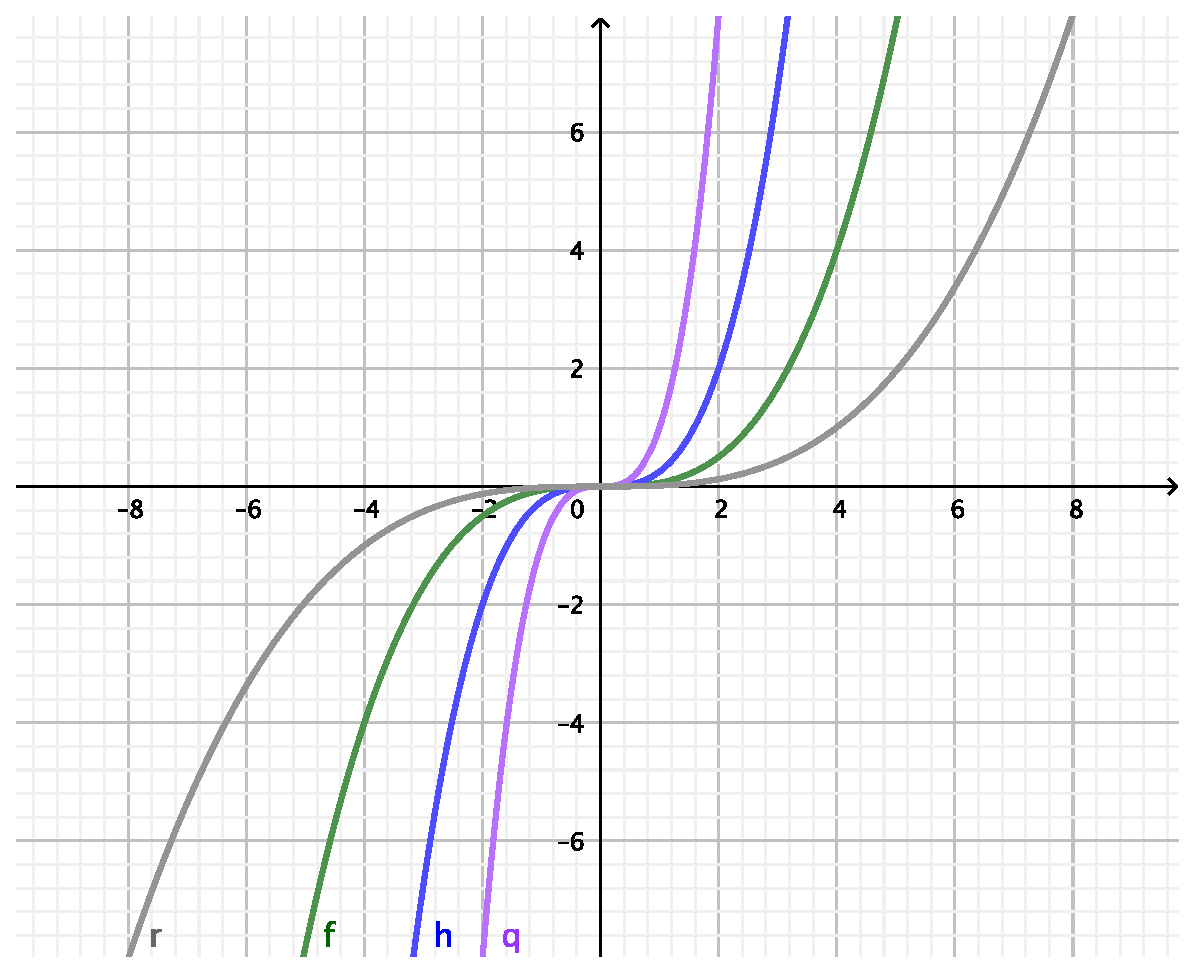
\includegraphics[height=12\baselineskip]{kap3/BundelFunktionenscharen.eps}
\end{minipage}

\subsection{Beispiel}

$f_{a}(x)= \dfrac{x^2-3ax}{x+a} \qquad \qquad D_{f} = \R \backslash \{ -a \}, \qquad a \in \R^+$ \\ �\\
Sei $K_{a}$ der Graph der Funktion.\\


\subsubsection{Bestimmen Sie die Schnittpunkte von $K_{a}$ mit den Koordinatenachsen}\\ \\

$f_{a}(0)=\dfrac{0}{x+a} = 0$ \\ \\ \\
\begin{array}{rcccl}
$\Rightarrow f_{a}(x)=0 & \Leftrightarrow & x^2-3x & = & 0 $\\
$&\Leftrightarrow & x(x-3a) & = & 0$ \\
$&\Leftrightarrow & x=0 & \lor & x  =  3a $ \\
\end{array}\\�\\�

Es ergeben sich die Punkte $P_{1}(0|0)$ und $P_{2}(3a|0)$\\\\

\subsubsection{Bestimmen Sie die Asymptoten von $K_{a}$}\\ \\

\begin{array}{rccccccl}
$ \Rightarrow & (x^2 & -3ax & +0) & : & (x+a) &=& x - 4a +\dfrac{4a^2}{x+a} \\ \\
& -(x^2 & +ax) & & & & & \\ \\
& & -4ax & +0 & & & & \\ \\
& & -(-4ax & -4a^2) & & & & \\ \\
& & & 4a^2 & & & &$ \\ \\
\end{array}\\ \\

Man erh"alt die schiefe Asymptote $y=x-4a$\\\\

Es liegt eine nicht hebbare Definitionsl"ucke bei $-a$ vor, daraus ergibt sich eine vertikale Asymptote $\Rightarrow x=-a$\\\\

 \subsubsection{Zeigen Sie $f''_{a}(x) = \frac{8a^2}{(x+a)^3}$}\\ \\

\begin{array}{rcl}
$f'_{a}(x) &=& \dfrac{(2x-3a)(x+a) - (x^2-3ax)(1)}{(x+a)^2} $\\
$&=& \dfrac{2x^2+2ax-3ax-3a^2-x^2-3ax}{x^2+2ax+a^2}$\\
$&=& \dfrac{x^2+2ax-3a^2}{(x+a)^2} $ \\ \\
$f''_{a}(x) &=& \dfrac{(\textcolor{red}{2x+2a})(x^2+2ax+a^2) - (x^2-2ax-3a^2)(2(\textcolor{red}{x+a}) ) }{(x+a)^{\textcolor{red}{4}}} $ \\
$ &=& \dfrac{2x^2+4ax+2a^2-2x^2+4ax+6a^2}{(x+a)^3}$\\
$&=& \dfrac{8a^2}{(x+a)^3}$
\end{array}

\subsubsection{Weisen Sie nach, dass $K_{a}$ genau einen Hochpunkt und genau einen Tiefpunkt besitzt. \\ Geben Sie die Koordinaten dieser Punkte in Abh"angigkeit von $a$ an und erstellen Sie eine Monotonietabelle der Funktionen $f_{a}$}\\ \\

Notwendige Bedingung f"ur Extremstellen: $\Rightarrow f'(x)=0 \\ \\
\Leftrightarrow x^2+2ax-3a^2 = 0 \qquad \qquad D= \R \backslash\{ -a \}  \\\\
\Rightarrow $\Delta$ = 4a^2 +12a^2 = 16a^2 \\ \\
\Leftrightarrow x_{1}=a \quad \lor \quad x_{2}=-3a \qquad \qquad L=\{a;-3a\}$ \\\\

$\Rightarrow f(a)=\dfrac{a^2-3a^2}{2a} = -a$\\\\
$\Rightarrow f(-3a)= \dfrac{9a^2+9a^2}{-2a} = -9a$ \\\\

Es ergeben sich somit die Extremstellen $H(-3a|-9a)$ und $T(a|-a)$. Bevor man mit der Monotonietabelle beginnt, muss die Polstelle untersucht werden.\\\\

\lim\limits_{x \rightarrow {-a^+}}{f_{a}} = \lim\limits_{x \rightarrow {-a^+}}{\dfrac{x^2-3ax}{x+a}} =\lim\limits_{h \rightarrow {0}}{\dfrac{(-a+h)^2 -3a(-a+h)}{(-a+h)+a}} = \lim\limits_{h \rightarrow {0}}{\dfrac{h^2-5ah+4a^2}{h}} = + \infty \\ \\

\lim\limits_{x \rightarrow {-a^-}}{f_{a}} = \lim\limits_{x \rightarrow {-a^-}}{\dfrac{x^2-3ax}{x+a}} =\lim\limits_{h \rightarrow {0}}{\dfrac{(-a-h)^2 -3a(-a-h)}{(-a-h)+a}} = \lim\limits_{h \rightarrow {0}}{\dfrac{h^2+5ah+4a^2}{-h}} = - \infty $\\ \\ \\
�
Jetzt kann die Monotonietabelle erstellt werden:\\\\

\begin{tikzpicture}
\tikzset{arrow style/.style = {blue,->,> = latex',
shorten > = 6pt,
shorten < = 6pt}}
\tkzTabInit{$x$ /1, $ x^2-2ax-3a $ /1.2, $(x+a)^2 $ /1.2, $f_{a}'(x)$ /1.2, $f_{a}(x)$ /3,}   {$-\infty$ ,$-3a$ , $-a$, $a$ ,$+\infty$}
\tkzTabLine{{},+,z,-,t,-,z,+,}
\tkzTabLine{{},+,t,+,d,+,t,+,}
\tkzTabLine{{},+,z,-,d,-,z,+,}
\tkzTabVar{ - / $-\infty$ , + / $H(-3a|-9a)$ / , -D+ / $-\infty$/$+\infty$  , - / $T(a|-a)$ , + / $+\infty$ }
\end{tikzpicture}\\ \\

\subsubsection{Zeigen Sie, dass es genau einen Punkt gibt, durch den alle Graphen $Ka$ gehen.}\\ \\

Diesen Punkt haben wir schon per ''Zufall'' herausgefunden, da wir eine Nullstelle gefunden haben, die nicht von $a$ abh"angt. Wenn man diesen aber nicht gefunden hat, geht man diesen L"osungsweg:\\\\

\begin{array}{rcccccl}
$\Rightarrow & f_{1}=f_{2} & \Leftrightarrow & \dfrac{x^2-3x}{x+1} & = & \dfrac{x^2-6x}{x+2} & \qquad \qquad D=\R \backslash \{-1;-2\} \\ \\
&&\Leftrightarrow& \dfrac{x-3}{x+1} &=& \dfrac{x-6}{x+2}&  \\\\
&&\Leftrightarrow& -x & = & -5x &\\ \\
&&\Leftrightarrow& x &=& 0 &�\qquad \qquad L=\{ 0 \} \\
$
\end{array}

\subsubsection{Bestimmen Sie $a\in \R^+$ so, dass der Graph $K_{a}$ durch den Punkt $P(5|\frac{5}{3})$ verl"auft}\\ \\

\begin{array}{rcccccl}
$\Rightarrow & f_{a}(5) = \dfrac{5}{3} & \Leftrightarrow & \dfrac{5^2-15a}{5+a} &=& \dfrac{5}{3} & \qquad \qquad D=\R \backslash \{-5\} \\\\
&&\Leftrightarrow & 15-9a &=& 5+a &\\\\
&&\Leftrightarrow & a&=&1&\qquad \qquad L=\{1\}$\\\\
\end{array}

\subsubsection{ Berechnen Sie die Schnittpunkte von $K_{1}$ mit der Geraden $j(x) =-15x -4$ }\\ \\

\begin{array}{rcccl}
$\Rightarrow  f_{1}(x) & = & \dfrac{x^2-3x}{x+1} &=& -15x-4 \quad = \quad y\\\\
&\Leftrightarrow & x^2-3x &=& -15x^2-19x-4\\\\
&\Leftrightarrow & 4x^2+4x+1 &=& 0\\\\
\Delta = 0 & \Rightarrow &x &=& -\dfrac{1}{2}$\\\\
\end{array}

$\Rightarrow f_{1}(-\dfrac{1}{2}) = \dfrac{(\frac{1}{2})^2 -3\cdot (\frac{1}{2})}{-\frac{1}{2}+1} = \dfrac{7}{2}$ \\ \\

Es existiert genau ein Schnittpunkt von $K_{1}$ mit der Geraden $j$: $P_{K_{1}j}(-\frac{1}{2}|\frac{7}{2})$

\subsubsection{ Vom Punkt $A(0|-4)$ wird die Tangente an $K_{1}$ gelegt. Bestimmen Sie eine Gleichung der Tangente und die Koordinaten des Ber"uhrpunktes }\\ \\

Sei $B(x_{0}|f_(x_{0}))$, dann lautet die Tangentengleichung:\\

\begin{array}{rccl}
$\Rightarrow & T_{x_{0}}(x) &=& f'(x_{0}) \cdot (x-x_{0}) +f(x_{0}) \\ \\
&&=& \dfrac{x_{0}^2 +2x_{0}-3}{(x_{0}+1)^2} \cdot (x-x_{0}) + \dfrac{x_{0}^2 -3x_{0}}{x_{0}+1} \\ \\
\end{array}

Jetzt werden die Koordinaten des Punktes $A(0|-4)$, durch den die Tangente auch noch geht, eingesetzt. \\

\begin{array}{rcccccl}
$\Rightarrow & T_{x_{0}}(0) &=& -4 & = & \dfrac{x_{0}^2 +2x_{0}-3}{(x_{0}+1)^2} \cdot (-x_{0}) + \dfrac{x_{0}^2 -3x_{0}}{x_{0}+1} &\qquad \qquad D=\R \backslash \{ -1\}$\\\\
$\Leftrightarrow &&& -4 (x_{0}+1)^2 &=& (x_{0}^2+2x_{0}-3)(-x_{0})+(x_{0}^2-3x_{0})(x_{0}+1) & $\\\\
$\Leftrightarrow &&& -4x_{0}^2-8x_{0}-4 &=& -x_{0}^3-2x_{0}^2+3x_{0}+x_{0}^3+x_{0}^2-3x_{0}^2-3x_{0}& $\\\\
$\Leftrightarrow &&& 4x_{0}^2+8x_{0}+4 &=& 4x_{0}^2&$\\\\
$\Leftrightarrow &&& x_{0} &=& -\dfrac{1}{2}&\qquad \qquad L=\left\{-\dfrac{1}{2}\right\}$\\\\
\end{array}

Nun werden die Koordinaten des Ber"uhrpunktes mit der Urspr"unglichen Funktion $f$ durch einsetzen errechnet. \\

$\Rightarrow f_{1}\left(-\dfrac{1}{2}\right) =  \dfrac{\left(-\frac{1}{2}\right)^2-3\cdot - \frac{1}{2}}{-\frac{1}{2}+1} = \dfrac{7}{2} $\\ \\

$\Rightarrow B\left(-\dfrac{1}{2}| \dfrac{7}{2} \right)$\\\\

Da es sich um eine Tangente handelt, muss nun die Steigung am Ber"uhrpunkt errechnet werden, um die Tangentengleichung bestimmen zu k"onnen. \\

$\Rightarrow f_{1}' \left(-\dfrac{1}{2}\right) = \dfrac{\left(-\frac{1}{2}\right)^2 +2\left(-\frac{1}{2}\right) -3 }{\left(-\frac{1}{2} \right)^2}  = -15$\\\\

Die Tangentengleichung lautet:\\ \\
$t(x) = -15x-4$\qquad \qquad mit \quad $D_{t}=\R$
\end{document}

  \chapter{Trigonometrie}
\@fleqntrue

\section{Kurze Wiederholung}
\begin{Definition}
  Im Kreis mit Radius 1 gelte:
  \begin{align*}
    \cos(\alpha)&= x_{_M}\\
    \sin(\alpha)&= y_{_M}\\
    \tan(\alpha)&=\dfrac {\sin(\alpha)} {\cos(\alpha)}
  \end{align*}
\end{Definition}\\
\definecolor{qqwuqq}{rgb}{0,0.39,0}
\definecolor{ttzzqq}{rgb}{0.2,0.6,0}
\definecolor{ffqqqq}{rgb}{1,0,0}
\definecolor{ttttff}{rgb}{0.2,0.2,1}
\definecolor{uququq}{rgb}{0.25,0.25,0.25}
\begin{tikzpicture}[line join=round,x=2.0833333333333335cm,y=2.0833333333333335cm]
  \draw[->,color=black] (-1.2,0) -- (1.2,0) node[below]{$x$};
  \foreach \x in {-1,1}
  \draw[shift={(\x,0)},color=black] (0pt,2pt) -- (0pt,-2pt) node[below] {\footnotesize $\x$};
  \draw[->,color=black] (0,-1.2) -- (0,1.2) node[left]{$y$};
  \foreach \y in {-1,1}
  \draw[shift={(0,\y)},color=black] (2pt,0pt) -- (-2pt,0pt) node[left] {\footnotesize $\y$};
  \draw[color=black] (0pt,-10pt) node[right] {\footnotesize $0$};
  \clip(-1.2,-1.2) rectangle (1.2,1.2);
  \draw [shift={(0,0)},color=qqwuqq,fill=qqwuqq,fill opacity=0.1] (0,0) -- (0:0.21) arc (0:57.13:0.21) -- cycle;
  \draw [line width=0.4pt] (0,0) circle (2.08cm);
  \draw (0,0)-- (0.54,0.84);
  \draw [line width=1.6pt,color=ttttff] (0,0.84)-- (0.54,0.84);
  \draw [line width=1.6pt,color=ffqqqq] (0.54,0.84)-- (0.54,0);
  \draw [line width=1.6pt,color=ttzzqq] (1,-1.2) -- (1,1.2);
  \begin{scriptsize}
    \fill [color=uququq] (0,0) circle (1.5pt);
    \draw[color=uququq] (-0.11,-0.11) node {$O$};
    \fill [color=black] (0.54,0.84) circle (1.5pt);
    \draw[color=black] (0.61,0.92) node {$M$};
    \fill [color=uququq] (0,0.84) circle (1.5pt);
    \draw[color=uququq] (0.03,0.94) node {$A$};
    \fill [color=uququq] (0.54,0) circle (1.5pt);
    \draw[color=uququq] (0.7,0.04) node {$B$};
    \draw[color=ttttff] (0.3,0.74) node {cos(α)};
    \draw[color=ffqqqq] (0.74,0.4) node {sin(α)};
    \draw[color=ttzzqq] (0.82,1.1) node {tan(α)};
    \draw[color=qqwuqq] (0.12,0.07) node {$\alpha$};
  \end{scriptsize}
\end{tikzpicture}
\\\\\\
Es ergeben sich folgende (wissenswerte) Werte:
\\
\begin{center}
  \begin{tabu} to 0.9\textwidth{| X[c] | X[c] | X[c] | X[c] | X[c] | X[c] | X[c] | X[c] | X[c] |}

    \hline
    & 0$^\circ$ & 30$^\circ$ & 45$^\circ$ & 60$^\circ$ & 90$^\circ$ & 180$^\circ$ & 270$^\circ$ & 360$^\circ$\\
    & 0 & $\dfrac{\pi}{6}$ & $\dfrac{\pi}{4}$ & $\dfrac{\pi}{3}$ & $\dfrac{\pi}{2}$ & \pi & $\dfrac{3\pi}{2}$ & $2\pi$\\
    \hline
    $\sin(\alpha)$ & 0 & $\dfrac{1}{2}$ & $\dfrac{1}{\sqrt{2}}$ & $\dfrac{\sqrt{3}}{2}$ & 1 & 0 & -1 & 0\\
    \hline
    $\cos(\alpha)$ & 1 & $\dfrac{\sqrt{3}}{2}$ & $\dfrac{1}{\sqrt{2}}$ & $\dfrac{1}{2}$ & 0 & -1 & 0 & 1\\
    \hline
    $\tan(\alpha)$ & 0 & $\dfrac{{1}}{\sqrt{3}}$ & 1 & $\sqrt{3}$ & X & 0 & X & 0\\
    \hline
  \end{tabu}

\end{center}
\section{Additions- und Verdopplungssätze}
\begin{Theorem}
  \begin{align*}
    \cos(a - b) & = \cos(a)\cos(b) + \sin(a)\sin(b)\\
    \sin(a - b) & = \sin(a)\cos(b) - \cos(a)\sin(b)\\
    \cos(a + b) & = \cos(a)\cos(b) - \sin(a)\sin(b)\\
    \sin(a + b) & = \sin(a)\cos(b) + \cos(a)\sin(b)
  \end{align*}
\end{Theorem}
\begin{Bemerkung}
  Hieraus ergeben sich einige weitere Relationen, wie z.B. $\sin(2a)$. Diese lassen sich jedoch schnell und leicht herleiten.
\end{Bemerkung}
\section{Allgemeine Sinus- und Kosinussätze}
In einem beliebigen Dreieck gelten abgewandelte Formen der aus der 8. Klasse bekannten Sätze:
\begin{Theorem}
  \begin{minipage}{0.6\textwidth}
    $\dfrac {a} {sin(\alpha)}=\dfrac {b} {sin(\beta)}=\dfrac {c} {sin(\gamma)}$\\\\
    $c^2=a^2+b^2-2abcos(\gamma)$
  \end{minipage}
  \begin{minipage}{0.4\textwidth}
    \definecolor{qqwuqq}{rgb}{0,0.39,0}
    \begin{tikzpicture}[line cap=round,line join=round,>=triangle 45,x=0.5cm,y=0.6cm]
      \clip(-0.4,-4.3) rectangle (9,3);
      \draw [shift={(4.22,1.92)},color=qqwuqq,fill=qqwuqq,fill opacity=0.1] (0,0) -- (-134.14:1.5) arc (-134.14:-47.61:1.5) -- cycle;
      \draw [shift={(-0.38,-2.82)},color=qqwuqq,fill=qqwuqq,fill opacity=0.1] (0,0) -- (1.04:1.5) arc (1.04:45.86:1.5) -- cycle;
      \draw [shift={(8.4,-2.66)},color=qqwuqq,fill=qqwuqq,fill opacity=0.1] (0,0) -- (132.39:1.5) arc (132.39:181.04:1.5) -- cycle;
      \draw (4.22,1.92)-- (8.4,-2.66);
      \draw (4.22,1.92)-- (-0.38,-2.82);
      \draw (8.4,-2.66)-- (-0.38,-2.82);
      \begin{scriptsize}
        \draw[color=black] (6.7,-0.44) node {$a$};
        \draw[color=black] (1.76,-0.08) node {$b$};
        \draw[color=black] (4.06,-2.28) node {$c$};
        \draw[color=qqwuqq] (4.4,1.05) node {$\gamma$};
        \draw[color=qqwuqq] (0.7,-2.45) node {$\alpha$};
        \draw[color=qqwuqq] (7.5,-2.2) node {$\beta$};
      \end{scriptsize}
    \end{tikzpicture}
  \end{minipage}
\end{Theorem}
\begin{Bemerkung}
  Man bemerkt, dass sich die bekannten Relationen ergeben, wenn einer der Winkel den Wert $\dfrac{\pi}{2}$ annimmt.
\end{Bemerkung}
\section{Sinusfunktionen}
Zur Vollständigen Funktionsdiskussion einer Sinus-Funktion sind einige Besonderheiten zu beachten:
\begin{enumerate}
  \item Amplitude und Periodizität\\
  Eine Funktion der Form $f(x)=a\cdot\sin(b(x-c))+d$ hat:
  \begin{itemize}
    \item die Periode $P = \dfrac{2\pi}{|b|}$
    \item die Amplitude $A = |a|$
    \item die Verschiebung entlang der $x$-Achse um $d$ und entlang der $y$-Achse um $c$
    \end{itemize}
  \item Symmetrieeigenschaften\\
  Hier sollte zumindest bekannt sein, dass $f(x)=\sin(x)$ punktsymmetrisch zum Origo ist, und dass $f(x)=\cos(x)$ Achsensymmetrisch zur $y$-Achse ist.
  \item Die Null-, Extrem- und Wendestellen sind in Form einer Menge anzugeben. (Es sei denn, die Aufgabenvorschrift fordert explizit zu einer Begrenzung auf ein angegebenes Intervall auf)\\
  \begin{Beispiel}
    Die Nullstellen der Funktion $f(x)=\sin(x)$ lassen sich dartstellen als: $x \in \{k\pi|k \in \Z\}$
  \end{Beispiel}
  \item Bei der Teilung durch eine Sinusfunktion können Definitionslücken an dessen Nullstellen entstehen. Auch diese können in der bereits gezeigten Form angegeben werden.
  \end{enumerate}
\section{Polarkoordinaten}
In der Kursstufe beschränken wir uns auf die Benutzung von Polarkoordinaten für Punkte in der Ebene (2D).
\begin{Definition}
  Polarkoordinaten sind eine Form der eindeutigen Punktangaben, doch anstatt wie kartesische Koordinaten 2 Entfernungen $x$ und $y$ zu verwenden, haben sie die Form $(r|\varphi)$. $r$ ist hierbei die Entfernung zum Origo und $\varphi$ ein orientierter Winkel (in $rad$).
\end{Definition}
\definecolor{zzzzzz}{rgb}{0.6,0.6,0.6}
\definecolor{ffqqqq}{rgb}{1,0,0}
\definecolor{qqzzqq}{rgb}{0,0.6,0}
\begin{tikzpicture}[line cap=round,line join=round,x=1.0cm,y=1.0cm]
  \draw[->,color=black] (-0.2,0) -- (2.64,0);
  \foreach \x in {,1,2}
  \draw[shift={(\x,0)},color=black] (0pt,-2pt);
  \draw[color=black] (2.47,0.04) node [anchor=south west] { x};
  \draw[->,color=black] (0,-0.29) -- (0,2.63);
  \draw[color=black] (0.05,2.43) node [anchor=west] { y};
  \clip(-0.2,-0.29) rectangle (2.64,2.63);
  \draw [shift={(0,0)},color=ffqqqq,fill=ffqqqq,fill opacity=0.1] (0,0) -- (0:0.41) arc (0:46.48:0.4) -- cycle;
  \draw [color=qqzzqq] (0,0)-- (2.05,2.16);
  \draw [color=zzzzzz] (0,2.16)-- (2.05,2.16);
  \draw [color=zzzzzz] (2.05,2.16)-- (2.05,0);
  \begin{scriptsize}
    \fill [color=black] (2.05,2.16) circle (1.5pt);
    \draw[color=black] (2.12,2.29) node {$P$};
    \draw[color=qqzzqq] (1.16,1.04) node {r};
    \draw[color=ffqqqq] (0.5,0.17) node {$\varphi$};
    \draw[color=zzzzzz] (0.96,2.02) node {y};
    \draw[color=zzzzzz] (1.9,1.03) node {x};
  \end{scriptsize}
\end{tikzpicture}
\subsection{Umrechnung}
\subsubsection{Kartesisch $\rightarrow$ Polar}
\begin{itemize}
  \item  $r=\sqrt{x^2+y^2}$
  \item $\varphi = \tan(\dfrac{y}{x})$
\end{itemize}
\subsubsection{Polar $\rightarrow$ Kartesisch}
\begin{itemize}
  \item $x = r\cdot\cos(\varphi)$
  \item  $y=r\cdot\sin(\varphi)$
\end{itemize}


\section{Beispiel einer Funktionsdiskussion}
Sei die Funktion $f(x)=2\cos(x)+2\sin(x)\cos(x)$, ihr Schaubild sei K.\\
Untersuchen Sie K im Intervall $[0;2\pi]$ auf gemeinsame Punkte mit der $x$-Achse, sowie Extrem- und Wendepunkte. Zeichnen Sie K im Intervall $[0;2\pi]$. Untersuchen Sie K auf Symmetrie.

\subsection{Definitionsmenge}
  $D=\R$

\subsection{Periodizität und Amplitude}
Die Periode von $f$ ist $P=2\pi$. Die Amplitude $A$ beträgt $\dfrac{3}{2}\sqrt{3}$.
\\

\begin{minipage}{0.5\textwidth}
  \subsection{Nullstellen}
  \subsubsection{Notwendige und hinreichende Bedingung:}
  \begin{align*}
    f(x)&=0\\
    \Leftrightarrow 2\cos(x)+2\sin(x)\cos(x)&=0\\
    \Leftrightarrow 2\cos(x)(1+\sin(x))&=0\\
    \stackrel{S.d.N}{\Rightarrow}
    \left\{\begin{array}{rccl}
      2\cos(x)&=&0&\\
      1+\sin(x)&=&0&
    \end{array}\right\\
    \Leftrightarrow
    \left\{ \begin{array}{rccl}
      \cos(x)&=&0&\\
      \sin(x)&=&-1&
    \end{array}\right\\
    \Leftrightarrow
    \left\{ \begin{array}{rccl}
      x_1&=&\dfrac{1}{2}\pi&\\\\
      x_2&=&\dfrac{3}{2}\pi&
    \end{array}\right\\
    \Rightarrow \mathbb{L}=\{(\dfrac{1}{2}\pi|0);(\dfrac{3}{2}\pi|0)\}
  \end{align*}
\end{minipage}
\vline
\begin{minipage}{0.5\textwidth}
  \subsection{Ableitungen}
    \begin{align*}
      f'(x)&=-2\sin(x)+2(\cos(x)\cos(x)-\sin(x)\sin(x))\\
      &=-2\sin(x)+2(\cos^2(x)-\sin^2(x))\\
      &=-2\sin(x)+2(1-\sin^2(x)-\sin^2(x))\\
      &=-4\sin^2(x)-2\sin(x)+2\\
      f''(x)&=-4(\cos(x)\sin(x)+\sin(x)\cos(x))-2\cos(x)\\
      &=-8\sin(x)\cos(x)-2\cos(x)\\
      f'''(x)&=-8(\cos(x)\cos(x)-\sin(x)\sin(x))+2\sin(x)\\
      &=-8(1-\sin^2(x)-\sin^2(x))+2\sin(x)\\
      &=16\sin^2(x)+2\sin(x)-8
    \end{align*}\\
\end{minipage}

\subsection{Extremstellen}
\begin{minipage}{0.5\textwidth}
  \subsubsection{Notwendige Bedingung:}
    f'(x)&=0\\
    \Leftrightarrow4\sin^2(x)-2\sin(x)+2&=0\\
    Substitution: y&=\sin(x)\\
    \Rightarrow4y^2-2y+2=0\\
    \stackrel{ABC-Formel}{\Rightarrow}y_{1,2}=\dfrac{2\pm\sqrt{(-2)^2-4*(-4)*2}}{-8}\\
    Resusbsitution:\\
    \Rightarrow
    \left\{\begin{array}{rccl}
      \sin(x)&=\dfrac{2+\sqrt{20}}{-8}\\
      \sin(x)&=\dfrac{2-\sqrt{20}}{-8}
    \end{array}\right\\
    \Rightarrow\mathbb{L}=\{\dfrac{1}{6}\pi;\dfrac{5}{6}\pi;\dfrac{3}{2}\pi\}
\end{minipage}
\vline
\begin{minipage}{0.5\textwidth}
  \subsubsection{Hinreichende Bedingung:}
  \begin{align*}
    f''(x)&\neq0\\
    \Rightarrow
    \left\{\begin{array}{rccl}
      f''(\dfrac{1}{6}\pi)&\stackrel{?}{=}0\\\\
      f''(\dfrac{5}{6}\pi)&\stackrel{?}{=}0\\\\
      f''(\dfrac{3}{2}\pi)&\stackrel{?}{=}0
    \end{array}\right\\
    \Leftrightarrow
    \left\{\begin{array}{rccl}
      8\sin(\dfrac{1}{6}\pi)\cos(\dfrac{1}{6}\pi)-2\sin(\dfrac{1}{6}\pi)&\stackrel{?}{=}0\\\\
      8\sin(\dfrac{5}{6}\pi)\cos(\dfrac{5}{6}\pi)-2\sin(\dfrac{5}{6}\pi)&\stackrel{?}{=}0\\\\
      8\sin(\dfrac{3}{2}\pi)\cos(\dfrac{3}{2}\pi)-2\sin(\dfrac{3}{2}\pi)&\stackrel{?}{=}0
    \end{array}\right\\
    \Leftrightarrow
    \left\{\begin{array}{rccl}
      8*\dfrac{1}{2}*\dfrac{\sqrt{3}}{2}-2*\dfrac{\sqrt{3}}{2}&\stackrel{!}{\neq}&0&,  <0 \Rightarrow HP\\
      8*\dfrac{1}{2}*-\dfrac{\sqrt{3}}{2}-2*-\dfrac{\sqrt{3}}{2}&\stackrel{!}{\neq}&0&,  >0 \Rightarrow TP\\
      8*(-1)(0)-2(0)&\stackrel{!}{=}&0& \Rightarrow \text{kein } EP
    \end{array}\right\\
  \end{align*}
\end{minipage}

\subsubsection{Ergebnis}
Auf dem Intervall $[0;2\pi]$  besitzt K den Hochpunkt H$(\dfrac{1}{6}\pi|f(\dfrac{1}{6}\pi))$ und den Tiefpunk T$(\dfrac{5}{6}\pi|f(\dfrac{5}{6}\pi))$.\\
$\Leftrightarrow$ H$(\dfrac{1}{6}\pi|\dfrac{3}{2}\sqrt{3})$ und T$(\dfrac{5}{6}\pi|-\dfrac{3}{2}\sqrt{3})$.
\subsection{Wendestellen}
\subsubsection{Notwendige Bedingung:}
\begin{align*}
  f''(x)=0\\
  \Leftrightarrow -8\sin(x)\cos(x)-2\cos(x)=0\\
  \Leftrightarrow \cos(x)(-2-8\sin(x))=0\\
  \stackrel{SdN}{\Rightarrow}
  \left\{\begin{array}{rccl}
    \cos(x)&=&0\\
    \sin(x)&=&-\dfrac{1}{4}
  \end{array}\right\\
  \Rightarrow \mathbb{L}=\{\dfrac{1}{2}\pi;\dfrac{3}{2}\pi;\sim3,394;\sim6,031\}
\end{align*}
\subsubsection{Hinreichende Bedingung:}

\begin{align*}
  f'''(x)&\neq0\\
  \Rightarrow
  \left\{\begin{array}{rccl}
    f'''(\dfrac{1}{2}\pi)&\stackrel{?}{=}0\\\\
    f'''(\dfrac{3}{2}\pi)&\stackrel{?}{=}0\\\\
    f'''(3,394)&\stackrel{?}{=}0\\\\
    f'''(6,031)&\stackrel{?}{=}0
  \end{array}\right\\
  \Leftrightarrow
  \left\{\begin{array}{rccl}
    16\sin^2(\dfrac{1}{2}\pi)+\sin(\dfrac{1}{2}\pi)-8&\stackrel{?}{=}0\\\\
    16\sin^2(\dfrac{3}{2}\pi)+\sin(\dfrac{3}{2}\pi)-8&\stackrel{?}{=}0\\
    16\sin^2(3,394)+\sin(3,394)-8&\stackrel{?}{=}0\\
    16\sin^2(6,031)+\sin(6,031)-8&\stackrel{?}{=}0
  \end{array}\right\\
  \Leftrightarrow
  \left\{\begin{array}{rccl}
    16*1+1-8&\stackrel{!}{\neq}&0&,>0\Rightarrow WP\\
    16*1-1-8&\stackrel{!}{\neq}&0&,>0,\text{ außerdem: } f'(\dfrac{3}{2}\pi)=0\Rightarrow Sattelpunkt\\
    -7,5&\stackrel{!}{=}&0&,<0\Rightarrow WP\\
    -7,5&\stackrel{!}{=}&0&,<0\Rightarrow WP&
  \end{array}\right\\
\end{align*}
\subsubsection{Ergebnis}
Auf dem Intervall $[0;2\pi]$  besitzt K die Wendepunkte $(\dfrac{1}{2}\pi|f(\dfrac{1}{2}\pi))$, $(3,394|f(3,394))$, $(6,031|f(6,031))$ und den Sattelpunkt $(\dfrac{3}{2}\pi|f(\dfrac{3}{2}\pi))$.\\
\Leftrightarrow $W_1(\dfrac{1}{2}\pi|0)$, $W_2(3,394|-1,452)$, $W_3(6,031|1,452)$, $S(\dfrac{3}{2}\pi|0)$.\\
\subsection{Schaubild}
\definecolor{ccqqqq}{rgb}{0.8,0,0}
\definecolor{cqcqcq}{rgb}{0.75,0.75,0.75}
\begin{tikzpicture}[line cap=round,line join=round,>=triangle 45,x=1.0cm,y=1.0cm]
  \draw [color=cqcqcq,dash pattern=on 1pt off 1pt, xstep=1.0cm,ystep=1.0cm] (-0.62,-3.28) grid (7.22,3.26);
  \draw[->,color=black] (-0.62,0) -- (7.22,0);
  \foreach \x in {,1,2,3,4,5,6,7}
  \draw[shift={(\x,0)},color=black] (0pt,-2pt) node[below] {\footnotesize $\x$};
  \draw[color=black] (7.04,0.04) node [anchor=south west] { x};
  \draw[->,color=black] (0,-3.28) -- (0,3.26);
  \foreach \y in {-3,-2,-1,1,2,3}
  \draw[shift={(0,\y)},color=black] (2pt,0pt) -- (-2pt,0pt) node[left] {\footnotesize $\y$};
  \draw[color=black] (0.05,3.05) node [anchor=west] { y};
  \draw[color=black] (0pt,-10pt) node[right] {\footnotesize $0$};
  \draw[color=ccqqqq] (1.5,2.5) node {K};
  \clip(-0.62,-3.28) rectangle (7.22,3.26);
  \draw[line width=1.6pt,color=ccqqqq, smooth,samples=100,domain=-0.6249016652708163:7.217846281536262] plot(\x,{2*cos(((\x))*180/pi)+2*sin(((\x))*180/pi)*cos(((\x))*180/pi)});
\end{tikzpicture}
\subsection{Symmetrie}
K ist punktsymmetrisch zu $W_1$, denn es gilt:
\begin{align*}
  f(\dfrac{1}{2}\pi+x)&=-1*f(\dfrac{1}{2}\pi-x)\\
  \Leftrightarrow
  2\cos(\dfrac{1}{2}\pi+x)+2\sin(\dfrac{1}{2}\pi+x)\cos(\dfrac{1}{2}\pi+x)&=-1*(2\cos(\dfrac{1}{2}\pi-x)+2\sin(\dfrac{1}{2}\pi-x)\cos(\dfrac{1}{2}\pi-x))\\
  \Leftrightarrow
  -2\sin(x)-2\cos(x)\sin(x)&=-1*(2\sin(x)+2\cos(x)\sin(x))
\end{align*}
K ist außerdem zu $S$ punktsymmetrisch, denn es gilt:
\begin{align*}
  f(\dfrac{3}{2}\pi+x)&=-1*f(\dfrac{3}{2}\pi-x)\\
  \Leftrightarrow
  2\cos(\dfrac{3}{2}\pi+x)+2\sin(\dfrac{3}{2}\pi+x)\cos(\dfrac{3}{2}\pi+x)&=-1*(2\cos(\dfrac{3}{2}\pi-x)+2\sin(\dfrac{3}{2}\pi-x)\cos(\dfrac{3}{2}\pi-x))\\
  \Leftrightarrow
  2\sin(x)+2\cos(x)\sin(x)&=-1*(-2\sin(x)-2\cos(x)\sin(x))
\end{align*}

  \chapter{Vektorielle Geometrie}


\section{Vektoren}
    \begin{Definition}
        Ein Vektor ist Element eines Vektorraums.
    \end{Definition}\\
    \paragraph{} Vektorräume, wir erinnern uns zurück. Verknüpfungen, inverse Elemente und die dazugehörenden Gesetze, konsequente Definitionen und mathematische Korrektheit, die guten alten Zeiten...\\
    Tatsächlich kann ein Vektor in den meisten Fällen als Verschiebung bezeichnet werden, \textbf{nicht aber als Pfeil oder Strich!}\\

    \subsection{Besondere Vektoren}

        \subsubsection{Der Ortsvektor}

            \paragraph{} Der Vektor von $O$ auf den Punkt $P$, geschrieben als $\vec{OP}$ oder $\vec{o}$.\\
            \paragraph{} Hat $P$ die Koordinaten $(P_1|P_2|...|P_n)$, so besitzt $\vec{o}$ die Darstellung $\left(\begin{array}{c} P_1 \\ P_2 \\ ...\\P_n\end{array}\right)$.

        \subsubsection{Der Nullvektor}

            \paragraph{} Der Vektor mit Wert $\left(\begin{array}{c} 0 \\ 0 \\ ...\\0\end{array}\right)$, er hat keine und alle Richtungen zugleich.
            \begin{Bemerkung}
                Er ist somit das neutrale Element der Vektoraddition.
            \end{Bemerkung}

        \subsubsection{Der Verbindungsvektor}

            \paragraph{} Der Vektor $\vec{AB}$ ist der Vektor, der den Punkt $A$ auf den Punkt $B$ abbildet. Er ist definiert als:\\ $\vec{AB}=\vec{OB}-\vec{OA}$, woraus folgt, dass: \begin{center} $\vec{AB} = \left(\begin{array}{c} b_1 - a_1 \\ b_2 - a_2 \\ ... \\ b_n - a_n \end{array}\right)$. \end{center}

        \subsubsection{Der Gegenvektor}

            \paragraph{} Der Gegenvektor zu $\vec{AB}$ ist $\vec{BA}$, definiert als  $-\vec{AB}$.
            \begin{Bemerkung}
                Er ist somit das inverse Element der Vektoraddition.
            \end{Bemerkung}

    \subsubsection{Der Einheitsvektor}

        \subsubsubsection{Norm eines Vektors}

            \paragraph{} Die Norm eines Vektors ist anschaulich als seine Länge zu interpretieren. Der Betrag, wie sie ebenfalls genannt wird, eines Vektors $\vec{v}$ ist folgendermaßen definiert: $\text{|}\vec{v}\text{|} = \sqrt{\displaystyle\sum_{i=1}^{n}v_{i^2}} ; \vec{v}\in\R^n$.
            \\
            \begin{tikzpicture}
                \draw[dashed, ->] (0,0,0) -- (0,0,3);
                \draw[dashed, ->] (0,0,0) -- (5,0,0);
                \draw[dashed, ->] (0,0,0) -- (0,3,0);
                \draw[dashed, color=red] (0,0,0) -- (5,0,3);
                \draw (0,0,3) -- (5,0,3) -- (5,3,3) -- (0,3,3) -- (0,0,3);
                \draw (0,3,3) -- (0,3,0) -- (5,3,0) -- (5,3,3);
                \draw (5,3,0) -- (5,0,0) -- (5,0,3);
                \draw[->, color=red] (0,0,0) -- (5,3,3);
                \draw (0,0,3.3) node {$x_1$};
                \draw (5.3,0,0) node {$x_2$};
                \draw (0,3.3,0) node {$x_3$};
                \draw (2.5,1.8,1.5) node [color=red]{$\vec{v}$};
                \draw (6.5,3,3) node [color=blue]{$P_1 (v_1, v_2, v_3)$};
                \draw (6.5,0,3) node [color=blue]{$P_2 (v_1, v_2, 0)$};
                \draw (1.7,0,1.9) node [color=red]{$\sqrt{v_1^{2}+v_2^{2}}$};
            \end{tikzpicture}
            \paragraph{} Anhand dieser Graphik lässt sich die Berechnung der Norm eines Vektors $\vec{v}\in\R^3$ verdeutlichen. Für diesen glit: $\text{|}\vec{v}\text{|}=\sqrt{v_1^{2}+v_2^{2}+v_3^{2}}$.
            \paragraph{} Ein Vektor, dessen Norm 1 beträgt wird als normiert oder Einheitsvektor bezeichnet. Für jeden Vektor $\vec{v}\in\R^{3}$ existiert ein Einheitsvektor $\vec{v^{*}}$ , der folgendermaßen definiert wird: $\vec{v^{*}}=\frac{1}{\text{|}\vec{v}\text{|}}*\vec{v}$.

\section{Linearkombination}

    \paragraph{} Vektoren lassen sich allgemein mit der additiven Verknüpfung des Vektorraumes verknüpfen. Diese Verknüpfung zwischen zwei beliebigen Vektoren $\vec{v}$ und $\vec{u}$ erfolgt, wie auch schon im Teil Verbindungsvektor gezeigt wird, wie folgt: $\vec{v}+\vec{u}=\left(\begin{array}{c}{v_1+u_1 \\ v_2+u_2 \\ ... \\ v_n+u_n}\end{array}\right)$.
    \\
    \begin{Definition}
       Eine Familie von Vektoren $\vec{a_1},\vec{a_2},...,\vec{a_n}\in V$ wird als linear abhängig bezeichnet, wenn die Gleichung: \\$r_1\cdot\vec{a_1}+r_2\cdot\vec{a_2}+...+r_n\cdot\vec{a_n}=\vec{0};r_i\in\R$ nicht nur die triviale Lösung $r_1=r_2=...=r_n=0$ besitzt. Existiert nur diese Lösung, ist die Familie linear unabhägig.
    \end{Definition}
    \paragraph{} Anders gesagt, ist eine Familie von Vektoren linear abhängig, wenn sich einzelne Vektoren dieser Familie als Linearkombination von einer beliebigen Anzahl anderer Vektoren der Familie darstellen lassen.
    \begin{Bemerkung}
      Eine linear abhängige Familie \textbf{aus genau zwei} Vektoren wird als kollinear bezeichnet.
      \\
      Eine linear abhängige Familie \textbf{aus genau drei} Vektoren, als komplanar.
    \end{Bemerkung}
\section{Basen und Erzeugendensystem}
    \paragraph{} Eine endliche Anzahl von Vektoren $\vec{a_1},\vec{a_2},...,\vec{a_n}\in V$ heißt Erzeugendensystem, wenn sich \texbf{jeder} Vektor $\vec{v}\in V$ als Linearkombination dieser Vektoren schreiben lässt. Um ein Erzeugendensystem zu bilden benötigt man mindestens die Anzahl Vektoren, die der Anzahl von Dimensionen von $\vec{v}$ entspricht. Wenn man \textbf{genau} diese Anzahl besitzt, spricht man von einer Basis.
    \subsection{Besondere Basen}
        \subsubsection{Orthogonalbasis}
        \paragraph{} Sind die Vektoren der Basis paarweise orthogonal zueinander, so spricht man von einer \textbf{Orthogonalbasis}.
        \subsubsection{Orthonormalbasis}
        \paragraph{} Sind die Vektoren zusätzlich zu dieser Bedingung normiert, wird sie als \textbf{Orthonormalbasis} bezeichnet. Die einfachste und meist benutzte Basis des $\R^3$ besteht aus den drei Vektoren $\vec{e_1}=\left(\begin{array}{c}{1\\0\\0}\end{array}\right),\vec{e_2}=\left(\begin{array}{c}{0\\1\\0}\end{array}\right),\vec{e_3}=\left(\begin{array}{c}{0\\0\\1}\end{array}\right)$. Sie wird als \textbf{Standardbasis} des $\R^3$ bezeichnet.
    \subsection{Basistransformation}

\section{Winkel zwischen Vektoren}\subsection{Orientierte Winkel}

\section{Geraden}
\section{Ebenen}
\section{Skalarprodukt}

  \chapter{Komplexe Zahlen}


\section{Einführung}

	\paragraph{} Die Ursache für die Einführung der komplexen Zahlen ist vergleichbar mit der jeglicher anderer Zahlenmengen (abgesehen
	von $\N$). Alles basiert auf einer Rechnung oder einer Menge an Rechnungen, welche für die vorhandenen Zahlenmengen \textbf{keine Lösung besitzen} oder aber diese Zahlenmengen einem nicht erlauben eine Lösung zu finden. Ein Beispiel hierfür ist die Einführung der
	negativen Zahlen. Gleichungen der Form $2 + x = 1$ waren eine Zeit lang nicht lösbar. Ebenso galt einmal, dass $x^2 - 2 = 0$ keine
	Lösung besitzt, da hierfür die reellen Zahlen benötigt werden. Analog dazu wird die Erweiterung auf die komplexen Zahlen begründet.
	Dies wird an folgendem klassischen Beispiel erläutert:

	\begin{align*}
		\qquad \qquad x^2 + 1 &= 0 \\
			\Leftrightarrow x &= \sqrt{-1} \quad \text{\Lightning}
	\end{align*}

	\paragraph{} Um dieser und anderen Gleichungen eine Lösung zuzuteilen ist es nicht nur notwendig die Zahlenmenge zu erweitern, sondern
	auch, neue Symbole und Zeichen einzuführen um die neuen Zahlen zu kennzeichnen. Für die $\Z$ ist es das Symbol \dq-\dq, für $\Q$
	\dq,\dq und $\dfrac{a}{b}$, für $\R$ $\sqrt{a}$ und die Zeichen $\pi$ und $e$ zum Beispiel (auch wenn beide sich anders darstellen lassen). (Ein) gewisse(r) Mathematiker (Leibniz glaube ich) hat entschieden, dass das einzige benötigte Zeichen $i$ sein sollte, da er sie imaginäre Zahl nannte (Für den Fall, dass ich hier ein bisschen was durcheinander bringe, sind Direktverbesserungen kommentarlos erlaubt und erwünscht).
 	Und dem war so, weshalb nun gilt:
											$$i \in \C : i^2 = -1; \C \definedBy \R \cup \left\{i\right\}$$

	\begin{Definition}
		Komplexe Zahlen werden standartmäßig mit dem Buchstaben $z$ dargestellt. Die allgemeine Formel einer solchen Zahl lautet:
		\\
		\begin{tikzpicture}
			\draw (0,0) node {" "};
			\draw (7.9, 0) node {$z = x + y \cdot i; x,y \in \R; i \in \C$};
			\draw[line width=0.8pt][decorate,decoration={brace,amplitude=3pt},rotate around={180:(7.6,-0.25)}] (7.6,-0.25) -- (8.1,-0.25);
			\draw[line width=0.8pt][decorate,decoration={brace,amplitude=2pt},rotate around={180:(6.7,-0.25)}] (6.7,-0.25) -- (7,-0.25);
		    \draw[line width=0.4pt] (6.55,-0.5) -- (5.1,-1.4) node[color=blue,left] {$Re(z)$};
		    \draw[line width=0.4pt] (7.35,-0.5) -- (9.2,-1.4) node[color=blue,right] {$Im(z)$};
		\end{tikzpicture}
		\\
		Hierbei wird $x = Re(z)$ Realteil und $y = Im(z)$ und zwar \textbf{nur $y$} Imaginärteil genannt.
	\end{Definition}

	\begin{Bemerkung}
		Eine Zahl $z = x + yi \in \C$ heißt rein imaginäre Zahl für $x = 0$. Analog dazu wird sie für $y = 0$ als reell bezeichnet.
	\end{Bemerkung}


\section{Der Körper der komplexen Zahlen}

	\paragraph{} Da wir nun wissen (oder halt auch nicht), weshalb wir die komplexen Zahlen benötigen, gilt es nun die verschiedenen Verknüpfungen, mit welchen wir zwei komplexe Zahlen verbinden, zu definieren. Wie alle anderen bekannten Mengen (außer $\N$), ist $\C$ teil eines \textbf{Körpers} welcher die zwei Verknüpfungen, denen wir allgemein die Namen \textbf{Addition} und \textbf{Multiplikation} geben. Das 3-Tupel (oder auch Tripel) ($\C$, +, *) ist somit der Körper, mit welchem wir arbeiten werden (jemals gefragt warum keine weiteren Verknüpfungen eingeführt wurden?). Jedoch muss auch erstmal bewiesen werden, dass dieses Tripel ein Körper ist:

	\begin{Beweis}
		\underline{\textbf{Die Addition}}:

		\paragraph{} Für die Addition gilt bekanntlich zu beweisen, dass ($\C$, $\oplus$) eine abelsche oder auch kommutative Gruppe ist:

		\begin{enumerate}[1)]
			\item \begin{align*}
						\forall z_1, z_2 \in \C: z_1 \oplus z_2 &\definedBy (x_1 + y_1i) \oplus (x_2 + y_2i) \\
														   		&= ((x_1 + x_2) + (y_1 + y_2)i) \\
														   		&\in \C \\
						\Rightarrow \forall z_1, z_2 \in \C: \oplus : \C \times \C \rightarrow \C & \quad \text{(Abgeschlossenheit)}
				  \end{align*}
			\item \begin{align*}
				  		(z_1 \oplus z_2) \oplus z_3 &= ((x_1 + x_2) + (y_1 + y_2)i) \oplus (x_3 + y_3i) \\
										  			&= ((x_1 + x_2 + x_3) + (y_1 + y_2 + y_3)i) \\
												    &= (x_1 + y_1i) \oplus ((x_2 + x_3) + (y_2 + y_3)i) \\
												    &= (x_1 + y_1i) \oplus ((x_2 + y_2i) \oplus (x_3 + y_3i)) \\
												    &= z_1 \oplus (z_2 \oplus z_3) \\
						\Rightarrow \forall z_1, z_2, z_3 \in \C: (z_1 + &z_2) \oplus  z_3 = z_1 \oplus (z_2 + z_3) \quad \text{(Assoziativität)}
				  \end{align*}
			\item \begin{align*}
						e = (0 + 0i) \in \C, \forall z \in \C:& \\
												   z \oplus e &= (x + yi) \oplus (0 + 0i) \\
													  		  &= ((x + 0) + (y + 0)i) \\
															  &= (x + yi) \\
															  &= z \\
						\Rightarrow \exists e: z \oplus e = z; z \in \C \quad &\text{(Neutrales Element)}
				  \end{align*}
			\item \begin{align*}
	  					z* = -(x + yi) \in \C, z \in \C \text{ (Hierbei gilt es z* nicht} & \text{mit $\overline{z}$ zu verwechseln)}: \\
								  z \oplus z* = (x + yi) \oplus (-(x + yi)) \text{          } & \\
								  			  = ((x - x) + (y - y)i) \text{ 				} & \\
											  = (0 + 0i) \text{ 							} & \\
											  = e \text{								    } & \\
						\Rightarrow \exists z*: z \oplus z* = e; z \in \C \quad \text{(Inverses Element)} \qquad &
	  			  \end{align*}
			\item \begin{align*}
						z_1 \oplus z_2 &= (x_1 + y_1i) \oplus (x_2 + y_2i) \\
									   &= ((x_1 + x_2) + (y_1 + y_2)i) \\
									   &= ((x_2 + x_1) + (y_2 + y_1)i) \\
									   &= (x_2 + y_2i) \oplus (x_1 + y_1i) \\
									   &= z_2 \oplus z_1 \\
						\Rightarrow \forall z_1, z_2 \in \C: z_1 \oplus z_2 = z_2 \oplus z_1 \quad \text{(Kom}&\text{mutativität)}
				  \end{align*}
		\end{enumerate}
		\newpage
		\underline{\textbf{Die Multiplikation}}:

		\paragraph{} Für die Multiplikation gilt ebenfalls zu beweisen, dass ($\C$, $\otimes$) eine kommutative Gruppe ist:

		\begin{enumerate}[1)]
			\item \begin{align*}
						\forall z_1, z_2 \in \C: z_1 \otimes z_2 &\definedBy (x_1 + y_1i) \otimes (x_2 + y_2i) \\
														   		 &= ((x_1x_2 - y_1y_2) + (x_1y_2 + x_2y_1)i) \\
														   		 &\in \C \\
						\Rightarrow \forall z_1, z_2 \in \C: \otimes : \C \times \C \rightarrow \C & \quad \text{(Abgeschlossenheit)}
				  \end{align*}
			\item \begin{align*}
				  		(z_1 \otimes z_2) \otimes z_3 &= ((x_1x_2 - y_1y_2) + (x_1y_2 + x_2y_1)i) \otimes (x_3 + y_3i) \\
										  			  &= ((x_1x_2x_3 - y_1y_2x_3 - x_1y_2y_3 - x_2y_1y_3) + (x_1x_2y_3 - y_1y_2y_3 + x_1y_2x_3 + x_2y_1x_3)i) \\
												      &= (x_1 + y_1i) \otimes ((x_2x_3 - y_2y_3) + (x_2y_3 + x_3y_2)i) \\
												      &= (x_1 + y_1i) \otimes ((x_2 + y_2i) \otimes (x_3 + y_3i)) \\
												      &= z_1 \otimes (z_2 \otimes z_3) \\
						\Rightarrow \forall z_1, z_2, z_3 \in \C: (z_1 + &z_2) \otimes  z_3 = z_1 \otimes (z_2 + z_3) \quad \text{(Assoziativität)}
				  \end{align*}
			\item \begin{align*}
						e = (1 + 0i) \in \C, \forall z \in \C:& \\
												   z \otimes e &= (x + yi) \otimes (1 + 0i) \\
													  		   &= ((1 \cdot x - 0 \cdot y) + (1 \cdot y + 0 \cdot x)i) \\
															   &= (x + yi) \\
															   &= z \\
						\Rightarrow \exists e: z \otimes e = z; z \in \C \quad &\text{(Neutrales Element)}
				  \end{align*}
			\item \begin{align*}
	  					z^{-1} = (x + yi)^{-1} \in \C, z \in \C:& \\
								  z \otimes z^{-1} &= (x + yi) \otimes \dfrac{1}{(x + yi)} \\
								  			  	   &= \dfrac{(x + yi) \cdot (x - yi)}{(x + yi) \cdot (x - yi)} \\
												   &= \dfrac{((x^2 + y^2) + (0i))}{((x^2 + y^2) + (0i))} \\
											  	   &= (1 + 0i) \\
											  	   &= e \\
						\Rightarrow \exists z^{-1}: z \otimes z^{-1} = e; z \in \C \quad \text{(Inverses Element)} \qquad &
	  			  \end{align*}
			\item \begin{align*}
						z_1 \otimes z_2 &= (x_1 + y_1i) \otimes (x_2 + y_2i) \\
									    &= ((x_1x_2 - y_1y_2) + (x_1y_2 + x_2y_1)i) \\
									    &= ((- y_1y_2 + x_1x_2) + (x_2y_1 + x_1y_2)i) \\
									    &= (x_2 + y_2i) \otimes (x_1 + y_1i) \\
									    &= z_2 \otimes z_1 \\
						\Rightarrow \forall z_1, z_2 \in \C: z_1 \otimes z_2 = z_2 \otimes z_1 \quad \text{(Kom}&\text{mutativität)}
				  \end{align*}
		\end{enumerate}
	\end{Beweis}

	\newpage

\section{Die Gauß'sche Zahlenebene}

	\paragraph{} Da jetzt der Körper der komplexe Zahlen definiert wurde, gilt es ihn nun in unser bekanntes Zahlensystem zu integrieren.
	Hierfür kann man zum Beispiel beobachten, wie sich komplexe Zahlen auf der \textbf{reellen Zahlengerade} (welche eine Veranschaulichung des euklidischen Vektorraums $\R^1$ ist) verhalten. Nun sollte erstmal der Begriff des \textbf{Zeiger}s eingeführt werden.
	\begin{Definition}
		Als Zeiger definieren wir ein visuelles Hilfsmittel, welches dem Darstellungsmodul eines Vektors, einem Pfeil, sehr ähnlich ist, jedoch sich durch eine kleine Nuance von Letzterem zu unterscheiden ist.
	\end{Definition}
	\\
	\begin{center}
		\begin{tikzpicture}[>=triangle 45]
			\draw[->,line width=0.8pt] (-5.5,0) -- (6,0);
			\foreach  \x in {-5,...,5}
    			\draw (\x,0.2) -- (\x,-0.2) node[below] {\x};
			\draw[->,line width=0.8pt,color=red] (0,0) -- (3,0);
		\end{tikzpicture}
	\end{center}
	\\
	\paragraph{} Zunächst muss verstanden werden, welche Transformation jeweils Addition und Multiplikation im $\R^1$ auf reelle Zahlen ausführt:
	\\
	\begin{center}
		\begin{tikzpicture}[>=triangle 45]
			\draw[->,line width=0.8pt] (-5.5,0) -- (6,0);
			\foreach  \x in {-5,...,5}
    			\draw (\x,0.2) -- (\x,-0.2) node[below] {\x};
			\draw[->,line width=1.3pt,color=red,dashed] (0,0) -- (3.3,0);
			\draw[->,line width=1.3pt,color=red] (0,0) -- (-3.3,0);
			\draw[line width=1.3pt,color=red] (1.5,0.6) node {3};
			\draw[line width=1.3pt,color=red] (-1.5,0.6) node {-3};
			\draw[->,color=red] (2.7,0) arc (0:180:2.7);
			\draw[line width=0.8pt,color=red] (0,3) node {180 \degree};
		\end{tikzpicture}
	\end{center}

  \chapter{Statistik und Wahrscheinlichkeit}

\section{Hypothesentests}

  \chapter{Arithmetik}
Nur ein weiterer kleiner Test\\
\section{Die Macht der Arithmetik}
Sie ist unglaublich star... Stärker als alle andere... Die Eine, um sie alle zu knechten... Sie ist mein $Scccchhhattzz$

  \documentclass[../MAIN/main.tex]{subfiles}
\begin{document}
\chapter{Matrizen}
\chapterauthor{Bruno}

	\section{Lineare Gleichungssysteme und Gaußalgorithmus}

Lineare Gleichungssysteme lassen sich aufwendig mit Einsetzungsverfahren oder Additionsverfahren l"osen, Carl Friedrich Gauß (1777-1855) hat ein Algorithmus erfunden, mit dem sie sich ohne Taschenrechner leicht und relativ schnell l"osen lassen.\\
Am Besten wird dieser mit einem Beispiel Erl"autert:\\
\\
$\Rightarrow$ $\left\{ \begin{array}{rccl}
4x+3y+z&=&13& (1)\\
2x-5y+3z& =& 1 &(2)\\
7x-y-2z&=&-1&(3)\\
\end{array}\right.$ \qquad \{ $1\cdot (1) -2\cdot (2)$ \}  und \{ $7\cdot (1) -4\cdot (3)$ \}  \qquad \qquad $D=\R^3$\\
\\
\\
Hier versucht man in Zeile (2) und (3) die erste Variabel zu eliminieren\\
\\
$\Leftrightarrow$ $\left\{ \begin{array}{rcl}
4x+3y+z&=&13\\
0x +13y -5z&=& 11\\
0x +25y +15z&=& 95\\
\end{array}\right.$ \qquad \{ $25\cdot(2) -13\cdot(3)$ \}  \\
\\
\\
Jetzt versucht man die zweite Variabel in der dritten Gleichung zu eliminieren\\
\\
$\Leftrightarrow$ $\left\{ \begin{array}{rcl}
4x+3y+z&=&13\\
0x +13y -5z&=& 11\\
0x+0y-320z&=&-960 $\qquad$ \Leftrightarrow z=3 \\
\end{array}\right.$\\
\\
\\
Jetzt wird eingesetzt\\
\\
$\Leftrightarrow$ $\left\{ \begin{array}{rcl}
4x+3y+z&=&13\\
0x+13y-5\cdot3&=&11 $\qquad$ \Leftrightarrow y=2\\
0x+0y+z&=&3\\
\end{array}\right.$\\
\\
\\
$\Leftrightarrow$ $\left\{ \begin{array}{rcl}
x+0y+0z&=&1\\
0x+y+0z&=&2\\
0x+0y+z&=&3\\
\end{array}\right.$\\
\\
\\
$\mathbb{L}=\{(1;2;3) \}$ Die Lösungsmenge wird als n-Tupel (geordente Objekte) alphabetisch sortiert.

	\section{LGS mit dem Taschenrechner l"osen}

	\subsection{Eindeutig l"osbare lineare Gleichungssysteme}

Ein lineares Gleichungssystem l"asst sich sehr viel schneller mit dem Taschgenrechner l"osen:\\

$\Rightarrow$ $\left\{ \begin{array}{rcl}
4x+3y+z&=&13\\
2x-5y+3z& =& 1\\
7x-y-2z&=&-1\\
\end{array}\right.$\\
\\
Hierf"ur geht man beim Taschenrechner auf [matrix] und auf [edit]. Dann gibt man seine Matrix (hier als Beispiel) ein:\\
\\
$\Rightarrow$ $\left\vert \begin{array}{rccl}
4&3&1&13\\
2&-5&3& 1 \\
7&-1&-2&-1\\
\end{array}\right\vert$\\
\\
Dann geht man wieder in den rechnen-Modus und gibt ein:  [matrix], dann geht man auf [math], [rref]. dann geht man nochmal auf [matrix], [A] (die gerade bearbeitete Matrix):\\
\\
$\Leftrightarrow$ $\left\vert \begin{array}{rccl}
1&0&0&1\\
0&1&0&2 \\
0&0&1&3\\
\end{array}\right\vert$ \qquad $\Rightarrow \mathbb{L}=\{(1;2;3) \}$ \\

Die L"osungsmenge wird als n-Tupel angegeben.\\
Wenn sich Werte mit Kommazahlen ergeben, ist es n"utzlich, im Taschenrechner [Math] $+$ [1](Frac) einzugeben, um sich die Werte in Br"uchen anzeigen zu lassen.\\

	\subsection{Nicht eindeutig l"osbare lineare Gleichungssysteme}

Oft begegnen einem auch unterbestimmte LGS, sei es in der Geometrie (Zwei Ebenengleichungen, die in einem Gleichungssystem als L"osung die Schnittgerade ergeben) oder in anderen Teilbereichen. Sie sind auch recht aufwendig von Hand zu l"osen, deshalb hier den schnelleren GTR-L"osungsweg:\\

$\Rightarrow$ $\left\{ \begin{array}{rcl}
x_{1}-2x_{2}+0x_{3}&=&10\\
x_{1}-x_{2}-x_{3}& =& 5\\
\end{array}\right.$\\
\\
Unterbestimmte LGS erkennt man daran, dass es mehr unbekannte als Gleichungen gibt:\\

$\Rightarrow$ $\left\vert \begin{array}{rccl}
1&-2&0&10\\
1&-1&-1& 5 \\
\end{array}\right\vert$\\
\\
\\
$\Leftrightarrow$ $\left\vert \begin{array}{rccl}
1&-2&0&10\\
0&0&1&5 \\
\end{array}\right\vert$  \qquad $\Rightarrow \mathbb{L}=\{(2t+10;t;t+5|t\in\R) \}$ \\

Auch hier wird die L"osungsmenge als n-Tupel angegeben, in Abh"angigkeit eines Faktors, dessen Wertebereich in der L"osungsmenge ebenfalls angegeben werden muss.\\\\
\end{document}

  \chapter{Algorythmik}
sdffzgkzgs\\


	\section{g}
fljzgkg\\

  \chapter{Integrale}
\section{Einführung}
Der Hauptunterschied zwischen einem bestimmten und einem unbestimmen Integral ist die Existenz (bestimmtes Integral) bzw. das Fehlen
(unbestimmtes Integral) der Integrationsgrenzen.\\
Bei einem bestimmten Integral ist die Lösung ein Flächeinhalt, also ein einfacher Zahlenwert.\\
Bei einem unbestimmten Integral erhält man als Lösung eine Funktion, eine sogenannte Stammfunktion.\\


\section{Bestimmte Integrale}
\begin{Definition}
  Wenn Integralgrenzen angegeben werden, handelt es sich um ein bestimmtes Integral:\\
  $
  \begin{array}{rcl}
    \int_{a}^{b} f(x)dx & = & \lim\limits_{n \rightarrow \infty} U_n = \lim\limits_{n \rightarrow \infty} s_n\\
                         & = & \lim\limits_{n \rightarrow \infty} O_n = \lim\limits_{n \rightarrow \infty} S_n\\
                         & = & \lim\limits_{n \rightarrow \infty} \dfrac{b-a}{n}\sum\limits_{k=1}^{n}f(\dfrac{b-a}{n}k)
  \end{array}
  $\\
  $S_n$ und $O_n$ bezeichnen die Obersumme, wohingegen $s_n$ und $U_n$ die Untersumme bezeichnen.
\end{Definition}
\begin{Bemerkung}
  $a$ und $b$ bezeichnen jeweils die untere und obere Grenze des zu berechnenden Integrals. Sie bezeichnen anschaulich die $x$-Werte, zwischen denen die Fläche berechnet wird.
\end{Bemerkung}
\begin{Bemerkung}
  Im allgemeinen Fall muss der Integrand $f(x)$ im Intervall $[a;b]$ stetig sein, damit das Integral bestimmt ist.
\end{Bemerkung}

\section{Stammfunktionen und der Hauptsatz der Differential- und Integralrechnung}
\begin{Definition}
  Eine Funktion $F$ heißt Stammfunktion der Funktion $f$, wenn $F'(x)=f(x)$
  gilt.\\
  Ist $F$ irgendeine Stammfunktion von $f$, dann ist auch $F(x)+C$ (mit
  konstantem $C$) eine Stammfunktion, denn beim Ableiten fällt $C$ als
  konstanter Summand weg. Jede Funktion hat also unendlich viele
  Stammfunktionen, die sich aber nur um einen konstanten Summanden
  unterscheiden.
\end{Definition}
\subsection{Sätze über Integrale}
\begin{Theorem}
  \begin{minipage}{0.6\textwidth}
    \begin{array}{rccl}
      $
      \int_a^b f(x)dx = -\int_b^a f(x)dx\\\\
      \int_a^b (f(x)+g(x))dx = \int_a^b f(x)dx + \int_a^b g(x)dx\\\\
      \int_a^b r*f(x)dx = r*\int_a^b f(x)dx\\\\
      \int_a^b f(x)dx + \int_b^c f(x)dx = \int_a^c f(x)dx
      $
    \end{array}
  \end{minipage}
  \begin{minipage}{0.4\textwidth}
    Invertieren der Intergrationsgrenzen\\\\
    Summenregel\\\\
    Linearität\\\\
    Abschnittweise Integration
  \end{minipage}

\end{Theorem}
\subsubsection{Beweise}
Invertieren der Intergrationsgrenzen:\\
$\int_a^b f(x)dx = F(b)-F(a) = -(F(a)-F(b)) = -\int_b^a f(x)dx$\\\\
Summenregel:\\
$\int_a^b f(x)+g(x)dx = [F(x)+G(x)]_a^b = F(b)+G(b)-(F(a)+G(b)) = F(b)-F(a)+G(b)-G(b) = \int_a^b f(x)dx$+\int_a^b g(x)dx$\\\\
Linearität:\\
$\int_a^b r*f(x)dx = [r*F(x)]_a^b = r*F(b)-r*F(a) = r*(F(a)-F(b)) = r*\int_a^b f(x)dx$\\\\
Abschnittweise Integration:\\
$\int_a^b f(x)dx+ \int_b^c f(x)dx = F(a)-F(b)-(F(b)-F(c)) = F(c)-F(a) = \int_a^c f(x)dx$\\\\

\subsection{Merkenswerte Integrale}
\begin{array}{rccl}
  \int x^n dx$&=&$\frac{x^{n+1}}{n+1}\\
  \int\sin x dx$&=&$ -\cos x\\
  \int\cos x dx$&=&$ \sin x\\
  \int\frac{ dx}{\cos^2x}$&=&$ \tan x\\
  \int\frac{1}{x} dx$&=&$ \ln|x|\\
\end{array}

\subsection{Integrationsregeln}
\subsubsection{Partielle Integration}
\begin{Definition}
  Seien $u$ und $v$ zwei stetig differenzierbare Funktionen im Intervall $I$ und $u'$
  und $v'$ in I stetig. Dann gilt:\\
  $\int u(x)'v(x) dx= u(x)v(x) - \int u(x)v'(x) dx$
\end{Definition}
Beweis:\\
Nachweisen u, v diffbar und u', v' stetig (kommt noch in sauber)\\
$
(u(x)*v(x))' = u'(x)v(x)+u(x)v'(x)\\
\Leftrightarrow \int (u(x)*v(x))' dx = \int u'(x)v(x)+\int u(x)v'(x)\\
\Leftrightarrow u(x)*v(x) = \int u'(x)v(x)+\int u(x)v'(x)\\
\Leftrightarrow \int u(x)v'(x) = u(x)*v(x)- \int u'(x)v(x)\\
$

Mit dieser Regel kann man \zB Integrale folgender Form lösen:
\[
\int x\sin x\dD x
\]
Setzt man hier $u'=\sin x$, $v=x$, dann ist $u=-\cos x$ und $v'=1$. Setzt man
diese Werte in die Produktintegrations-Formel ein, dann folgt:
\begin{align*}
\int x\sin x\dD x&= (-\cos x)x-\int (-\cos x)\cdot1\dD x\\
&=-x\cos x+\int\cos x\dD x= -x\cos x+\sin x
\end{align*}

Ein anderes schönes Beispiel ist die Stammfunktion von $\ln x$. Dazu fasst man
$\ln x$ als $1\cdot\ln x$ auf und wählt $u'=1$, $v=\ln x$, also $u=x$ und
$v'=1/x$ und erhält:
\[
\int\ln x\dD x=x\ln x-\int x\cdot\frac{1}{x}\dD x=
x\ln x-\int 1\dD x=x\ln x -x
\]

\subsubsection{Substitutionsmethode}
Es soll die Stammfunktion von $x(1-x^2)^9$ bestimmt werden. Hier wäre zum
Ableiten die Kettenregel und die Produktregel nötig, beides gibt es aber in
reiner Form beim Integrieren nicht. Man kann aber häufig durch geschickte
Substitution das Integral auf eine Form bringen, für die dann eine
Stammfunktion angegeben werden kann. Der wesentliche Punkt dabei ist, dass
nicht nur $x$ sondern auch $\dD x$ der Substitution unterworfen werden muss.

In diesem Beispiel setzen wir $u=1-x^2$. Dann ist $\dD u=u'(x)\dD x=-2x\dD x$.
Somit ist $\dD x=-\dD u/2x$. Nun geht's los:
\[
\int x(1-x^2)^9\dD x=\int x u^9 \frac{-1}{2x}\dD u
=-\frac{1}{2}\int u^9\dD u=-\frac{1}{20}u^{10}=-\frac{1}{20}(1-x^2)^{10}
\]

Hätten wir hier die Stammfunktion nicht benötigt, sondern nur den Wert eines
bestimmten Integrals, dann hätte man sich die Rücksetzung sparen können, indem
man die Grenzen auf die neue Variable umschreibt:
\[
\int_{x=0}^1 x(1-x^2)^9\dD x=-\frac{1}{2}\int_{u=1}^0u^9\dD u
=-\frac{1}{20}\left[u^{10}\right]_1^0=-\frac{1}{20}(0-1)=\frac{1}{20}
\]

In diesem Beispiel haben wir einen Teilausdruck des Integrals gleich $u$
gesetzt. Im folgenden Beispiel machen wir es anders herum und setzen $x$
gleich einer Funktion von $u$. Es soll die Fläche einer Ellipse berechnet
werden. Für den oberen Ellipsenbogen gilt die Gleichung (Auflösen der
Mittelpunktsform~\eqref{eq:7} nach $y$):
\[
y=\frac{b}{a}\sqrt{a^2-x^2}
\]
Die Fläche unter dem oberen Ellipsenbogen ist die halbe Ellipsenfläche und
berechnet sich so:
\[
A=\int\limits_{x=-a}^a \frac{b}{a}\sqrt{a^2-x^2}\,\dD x=
\int\limits_{u=-\frac{\pi}{2}}^{\frac{\pi}{2}}
\frac{b}{a}\sqrt{a^2-a^2\sin^2u}\,a\cos u\,\dD u=
\int\limits_{-\frac{\pi}{2}}^{\frac{\pi}{2}}ab\cos^2u\,\dD u
\]
Dabei hat man $x=a\sin u$ gesetzt, dann wird $\dD x=a\cos u \dD u$. Nun muss
man nur noch die Stammfunktion von $\cos^2u$ ermitteln. Dazu kann man etwa die
Beziehung $\cos2u=2\cos^2u-1$ heranziehen, also
$\cos^2u=\frac{1}{2}(1+\cos2u)$. Diese hat die Stammfunktion
$\frac{1}{2}(u+\sin u\cos u)$. Damit bekommt man für die Fläche:
\[
A=\frac{ab}{2}\left[u+\sin u\cos u\right]_{-\frac{\pi}{2}}^{+\frac{\pi}{2}}=
\frac{ab}{2}[(\frac{\pi}{2}+0)-(-\frac{\pi}{2}+0)]=\frac{1}{2}\pi a b
\]
Die gesamte Fläche der Ellipse ist doppelt so groß, also $\pi a b$.

\subsubsection{Partialbruchzerlegung}
Die Partialbruchzerlegung ist ein allgemeines Verfahren zur Integration
gebrochen rationaler Funktionen. Es sei gegeben:
\begin{equation}
  \label{eq:68}
  f(x)=\frac{P(x)}{Q(x)}
  =\frac{a_0+a_1x+\dots+a_nx^n}{b_0+b_1x+\dots+b_mx^m}
\end{equation}
Im Falle $m\le n$ führt man zuerst eine Polynomdivision aus, dann bekommt man
eine ganzrationale Funktion und eine gebrochen rationale mit $m>n$, so dass
wir uns für das Weitere auf den Fall $m>n$ beschränken können.

Das Nennerpolynom kann im Komplexen vollständig in Linearfaktoren zerlegt
werden, im Reellen bleiben ggf. quadratische Faktoren übrig, die keine reellen
Nullstellen mehr haben. Seien nun $x_k$ die Nullstellen von $Q(x)$ mit der
Vielfachheit $\nu_k$ dann kann man $Q(x)$ stets auf die folgende Form bringen:
\begin{equation}
  \label{eq:69}
  Q(x)=b_m(x-x_1)^{\nu_1}(x-x_2)^{\nu_2}\dots(x-x_k)^{\nu_k}
  (x^2+\alpha_1x+\beta_1)^{\mu_1}\dots(x^2+\alpha_rx+\beta_r)^{\mu_r}
\end{equation}
Die gebrochen rationale Funktion $f(x)$ lässt sich nun als Summe von
Partialbrüchen schreiben. Dabei gilt:
\begin{enumerate}
\item Jeder Linearfaktor $(x-x_k)$ der Vielfachheit $\nu_k$ trägt zur
  Zerlegung die folgenden Summanden bei:
  \[
  \frac{A_1}{(x-x_k)}+\frac{A_2}{(x-x_k)^2}+\dots
  +\frac{A_{\nu_k}}{(x-x_k)^{\nu_k}}
  \]
\item Jeder quadratische Faktor mit der Vielfachheit $\mu_k$ trägt die
  folgenden Summanden bei:
  \[
  \frac{C_1x+D_1}{(x^2+\alpha x+\beta)}+
  \frac{C_2x+D_2}{(x^2+\alpha x+\beta)^2}+\dots+
  \frac{C_{\mu_k}x+D_{\mu_k}}{(x^2+\alpha x+\beta)^{\mu_k}}
  \]
\end{enumerate}

\noindent Die Linearfaktoren lassen sich sofort integrieren, bei den
quadratischen geht man so vor:
\[
(x^2+\alpha x+\beta)=\bigl(x+\tfrac{\alpha}{2}\bigr)^2+\delta^2
=(\delta y)^2+\delta^2=\delta^2(y^2+1)
\]
Hier hat man quadratisch ergänzt und $\delta\cdot y=x+\frac{\alpha}{2}$
substituiert. Mit dieser Substitution ist
\[
x=\delta y-\frac{\alpha}{2}\qquad y=\frac{x+\frac{\alpha}{2}}{\delta}\qquad
\dD x=\delta\dD y
\]
Nun wird das Integral zu:
\begin{align*}
  \int\frac{Cx+D}{(x^2+\alpha x+\beta)^\mu}\dD x
  &=\frac{1}{\delta^{2\mu-1}}
  \int\frac{C\delta y+D-\frac12C\alpha}{(y^2+1)^\mu}\dD y\\
  &=\frac{C}{\delta^{2\mu-2}}\int\frac{y\dD y}{(y^2+1)^\mu}
  +\frac{D-\frac12C\alpha}{\delta^{2\mu-1}}\int\frac{\dD y}{(y^2+1)^\mu}
\end{align*}
Für das erste der beiden verbleibenden Integrale bekommt man dann
\begin{equation}
  \label{eq:70}
  \int\frac{y\dD y}{(y^2+1)^\mu}=\frac12\int\frac{\dD u}{u^\mu}=
  \begin{cases}
    \dfrac{u^{1-\mu}}{2(1-\mu)}=&\text{für~}\mu=2, 3, \dots\\
    \frac{1}{2}\ln|u|& \text{für~} \mu=1
  \end{cases}
\end{equation}
Hier hat man $u=y^2+1$ gesetzt. Nun muss noch das zweite bestimmt werden.
\[
J_\mu=\int\frac{\dD y}{(y^2+1)^\mu}
\]
Für $\mu=1$ ist es bekannt, $J_1=\arctan y$.

Wir werden eine Rekursionsformel für die $J_\mu$ herleiten. Wir beginnen mit
der Beziehung
\[
J_{\mu+1}=\int\frac{(y^2+1)-y^2}{(y^2+1)^{\mu+1}}\dD y
=J_\mu-\int\frac{y^2}{(y^2+1)^{\mu+1}}\dD y
\]
Nun denken wir uns den zweiten Integranden als $y\cdot$Rest geschrieben und
integrieren partiell:
\[
\int y\cdot\frac{y\dD y}{(y^2+1)^{\mu+1}}=
\frac{-y}{2\mu(y^2+1)^\mu}+\frac{1}{2\mu}\int\frac{\dD y}{(y^2+1)^\mu}=
\frac{-y}{2\mu(y^2+1)^\mu}+\frac{1}{2\mu}\,J_\mu
\]
Setzt man das oben ein, so bekommt man die Rekursionsformel:
\begin{equation}
  \label{eq:71}
  J_{\mu+1}=\left(1-\frac{1}{2\mu}\right)J_\mu+\frac{y}{2\mu(y^2+1)^\mu}
\end{equation}
Insbesondere ist dann (rechne das nach!)
\begin{align*}
  J_1&=\arctan y\\
  J_2&=\frac{1}{2}\arctan y+\frac{y}{2(y^2+1)}\\
  J_3&=\frac38\left(\arctan y+\frac{y}{y^2+1}\right)+\frac{y}{4(y^2+1)^2}\\
  J_4&=\frac{5}{16}\left(\arctan y+\frac{y}{y^2+1}\right)+
       \frac{5}{24}\cdot\frac{y}{(y^2+1)^2}+\frac{y}{6(y^2+1)^3}
\end{align*}

\subsection{Bemerkungen}
Erweiterung der NEW-Regel

\section{Flächenberechnung mittels Integralen}
\begin{Definition}
  Für die auf dem Intervall $[a;b]$ (also stückweise) stetige Funktion $f$ mit Nullstellen und $x_1,x_2,...,x_n$
  mit $a \leq x_1 \leq x_2 \leq ... \leq x_n \leq b$ ist der Flächeninhalt $A$ zwischen dem Graphen von $f$ und
  der $x_1$-Achse im Intervall $[a;b]$ gegeben durch:\\\\
  $A= |{\int_a^{x_1} f(x)dx}|+|{\int_{x_1}^{x_2} f(x)dx}|...+|{\int_{x_{n-1}}^{x_n} f(x)dx}|+|{\int_{x_n}^b f(x)dx}|$
\end{Definition}

\\Graph+Intergal
\definecolor{xdxdff}{rgb}{0.49019607843137253,0.49019607843137253,1.}
\definecolor{ffqqqq}{rgb}{1.,0.,0.}
\definecolor{qqzzqq}{rgb}{0.,0.6,0.}
\begin{tikzpicture}[line cap=round,line join=round,>=triangle 45,x=5.0cm,y=5.0cm]
  \begin{axis}[
  x=5.0cm,y=5.0cm,
  axis lines=middle,
  xmin=-1.0261085461981427,
  xmax=0.8799969446433364,
  ymin=-0.45014188815180656,
  ymax=0.9656470777143747,
  xtick={-1.0,-0.8,...,0.8},
  ytick={-0.4,-0.2,...,0.8},]
  \clip(-1.0261085461981427,-0.45014188815180656) rectangle (0.8799969446433364,0.9656470777143747);
  \draw[line width=0.8pt,color=ffqqqq,fill=ffqqqq,fill opacity=0.10000000149011612] plot[raw gnuplot, id=func1] function{set samples 100; set xrange [-0.7:0.4]; plot 7.0*x**(3.0)+5.0*x**(2.0)-0.3} -- (0.4,0.) -- (-0.7,0.) -- cycle;
  \draw[line width=2.4pt,color=qqzzqq] plot[raw gnuplot, id=func0] function{set samples 100; set xrange [-0.9261085461981428:0.7799969446433365]; plot 7.0*x**(3.0)+5.0*x**(2.0)-0.3};
  \begin{scriptsize}
  \draw[color=qqzzqq] (-0.836110892770214,-1.1411817405388711) node {$f$};
  \draw[color=xdxdff] (-0.6828869787154327,0.05702926736952031) node {$A$};
  \draw[color=xdxdff] (0.4203252024789926,0.05702926736952031) node {$B$};
  \end{scriptsize}
  \end{axis}
\end{tikzpicture}
\begin{Beispiel}
  $f(x)=x^2-2x^3;x\in \R$\\
  notwendige und hinreichende Bedingung für Nullstellen:$f(x)=0$\\
  $\Leftrightarrow x^2(x-2)&=0\\
  \stackrel{SdN}{\Leftrightarrow}
  \left\{ \begin{array}{rcl}
  x^2&=0\\
  x-2&=0
  \end{array}\right\\
  \Leftrightarrow
  \left\{ \begin{array}{rcl}
  x_1&=0\\
  x_2&=2
  \end{array}\right\\
  $\\
  Also gilt:\\
  $A_{-1}^{3} &= |\int_{-1}^0 x^3-2x^2 dx| + |\int_{0}^2 x^3-2x^2 dx| + |\int_{2}^3 x^3-2x^2 dx|\\
  &= |\Big[\dfrac{1}{4}x^4-\dfrac{2}{3}x^3\Big]_{-1}^0| + |\Big[\dfrac{1}{4}x^4-\dfrac{2}{3}x^3\Big]_{0}^2| + |\Big[\dfrac{1}{4}x^4-\dfrac{2}{3}x^3\Big]_{2}^3|\\
  &= |0-(\dfrac{1}{4}-\dfrac{2}{3})| + |4-\dfrac{8}{3}-0| + |\dfrac{81}{4}-54 - (4-\dfrac{8}{3})|\\
  &= \dfrac {35}{6}$FE\\
  (Also hoffentlich)

\end{Beispiel}
\begin{GTR-Tipp}
  Mit $Y_1 = f(x)$ und $Y_2 = abs(Y_1)$ bzw. $Y_2 = |Y_1|$ (zu finden in 'MATH'>'NUM' oder über Alpha-F2) lässt sich die Fläche berechnen über 2nd-CALC mit der Option Integral.\\
  Hierzu wählt man $Y_2$ aus und gibt $a$ und $b$ an.
\end{GTR-Tipp}

  \chapter{Exponentialfunktionen}

\begin{Definition}
Man bezeichnet als Exponentialfunktion eine Funktion der Form $x\rightarrow a^x$ mit $a\in \R^+\backslash 1$\\
$x$ ist die Variable und wird \textit{Exponent} oder \textit{Hochzahl} genannt.\\
$a$ nennt man \textit{Basis} oder \textit{Grundzahl}, sie ist für jede Funktion fest forgegeben.\\\\
Allgemeiner gilt jede Funktion, bei der die Variable im Exponenten steht als Exponentialfunktion. 
\end{Definition}




		\section{Wiederholung: Potenzgesetze}
Seien $a$, $b\in\R$, sowie $n$, $m\in\N$, dann gilt:
\begin{enumerate}
\begin{minipage}{0.5\textwidth}
\item$a^0=1$ (für $a\neq 0$)
\item$a^1=a$
\item$a^n=\underbrace{a\cdot a\cdot ... \cdot a}_{n Mal}$
\item$a^m\cdot a^n=a^{m+n}$
\item$(a^n)^m=a^{n\cdot m}$
\end {minipage}
\begin{minipage}{0.5\textwidth}
\item$a^{-n}=\dfrac{1}{a^n}$
\item$\dfrac{a^n}{a^m}=a^{n-m}$
\item$\left(\dfrac{a}{b}\right)^n=\dfrac{a^n}{b^n}$
\item $a^{\frac{1}{n}}=\sqrt[n]{a}$
\item$a^{\frac{m}{n}}=\sqrt[n]{a^m}$
\end {minipage}
\end{enumerate}

		\section{Die Eulersche Zahl ($e$)}

\begin{Definition}
	$e = 2,71828182845904523536028747135266249775724709369995...$\\
	\\
	Die \textbf{Eulersche Zahl} ($e$) ist eine irrationale, transzendente und reelle Zahl, die die Basis des (natürlichen) 			Logarithmus und der (natürlichen) Exponentialfunktion ist.\\
	Die Darstellung, der man am Häufigsten begegnet ist diese:
	$e=\lim\limits_{t\to \infty}\left(1+\dfrac{1}{t}\right)^t;t\in\R$
\end{Definition}
\\\\
Benannt nach dem bekannten Mathematiker Leonhard Euler ist diese Zahl eine der wichtigsten Konstanten der Mathematik.
Sie ist die Basis des natürlichen Logarithmus und der natürlichen Exponentialfunktion. Diese besondere Exponentialfunktion wird aufgrund dieser Beziehung zur Zahl $e$ häufig kurz $e$-Funktion genannt, sie eignet sich zur Modellierung von Wachstums- und Zufallsprozessen.\\

\begin{Bemerkung}
	Eine alternative Definition wäre folgende:
	Die positive Zahl $a$, für die die Exponentialfunktion $f$ mit $f(x)=a^x$  mit ihrer Ableitungsfunktion $f'$ übereinstimmt, 		heißt Eulersche Zahl. (siehe 12.5)
\end{Bemerkung}
\\
\begin{Definition}
  Eine reelle Zahl heißt (oder allgemeiner eine komplexe Zahl) transzendent,
  wenn sie nicht Nullstelle eines Polynoms mit ganzzahligen Koeffizienten ist.
  Andernfalls handelt es sich um eine algebraische Zahl. Jede reelle transzendente Zahl ist überdies irrational.
\end{Definition}

	\subsection{Verschiedene Darstellungen}

$e$ ist darstellbar bzw. ergibt sich durch:
\begin{itemize}
\item $\sum\limits_{k=0}^{\infty}\dfrac{1}{k!}$
\item $\lim\limits_{t\to \infty}\left(1+\dfrac{1}{t}\right)^t;t\in\R$
\item $\lim\limits_{n\to \infty}\left(1+\dfrac{1}{n}\right)^n;n\in\N$
\end{itemize}

	\subsection{Herleitung zur Zahl $e$}

Wir definieren eine Folge $(e_{n})n\in\N$ durch $e_{n}=\left(1+\dfrac{1}{n}\right)^n$ und beweisen ihre Konvergenz.

\begin{itemize}

\item\begin{align*}\dfrac{e_{n+1}}{e_{n}}&=\dfrac{{\left(1+\dfrac{1}{n+1}\right)}^{n+1}}{{\left(1+\dfrac{1}{n}\right)}^{n}}\\
&=\left(\dfrac{n(n+2)}{(n+1)^2}\right)^{n+1}\cdot\left(1+\dfrac{1}{n}\right)\\
&=\textcolor{blue}{\left(1-\dfrac{1}{(n+1)^2}\right)^{n+1}}\cdot\textcolor{red}{\dfrac{n+1}{n}}
\end{align*}

\item Die Umformung ermöglicht uns auf den Term $\left(1-\dfrac{1}{(n+1)^2}\right)^{n+1}$ die Ungleichung von Bernoulli anzuwenden. Diese besagt Folgendes: $(1+x)^n>1+nx$ für $n\geq2$ und $x>-1$\\
\begin{align*}\Rightarrow\textcolor{blue}{\left(1-\dfrac{1}{(n+1)^2}\right)^{n+1}}&\textcolor{blue}{>} 1+(n+1)\cdot\left(-\dfrac{1}{(n+1)^2}\right)\\
&=1-\dfrac{1}{n+1}\\
&=\textcolor{blue}{\dfrac{n}{n+1}}
\end{align*}

\item Dies kann man für den ersten Ausdruck verwenden:\\
\begin{align*}
\Rightarrow\dfrac{e_{n+1}}{e_{n}}&=\left(1-\dfrac{1}{(n+1)^2}\right)^{n+1}\cdot\dfrac{n+1}{n}\\
&\textcolor{blue}{>\dfrac{n}{n+1}}\cdot\textcolor{red}{\dfrac{n+1}{n}}\\
&=1
\end{align*}
\textbf{$\Leftrightarrow e_{n}$ ist streng monoton steigend}
\end{itemize}

Sei eine Folge $f_{n}$ mit $f_{n}=\left(1+\dfrac{1}{n}\right)^{n+2}$, deren Monotonieverhalten wir untersuchen wollen.\\
Dazu formen wir den Term so um, dass die Bernoulli-Ungleichung angewandt werden kann.

\begin{itemize}
\item\begin{align*}\dfrac{f_{n}}{f_{n+1}}&=\dfrac{\left(1+\dfrac{1}{n}\right)^{n+1}}{\left(1+\dfrac{1}{n}\right)^{n+2}}\\
&=\left(\dfrac{1+\dfrac{1}{n}}{1+\dfrac{1}{n+1}}\right)^{n+2}\cdot\dfrac{1}{1+\dfrac{1}{n}}\\
&=\left(\dfrac{\dfrac{n+1}{n}}{\dfrac{n+2}{n+1}}\right)\cdot\dfrac{n}{n+1}\\
&=\left(\dfrac{(n+1)^2}{n(n+2)}\right)^{n+2}\cdot\dfrac{n}{n+1}\\
&=\left(\dfrac{n^2+2n+1}{n^2+2n}\right)^{n+2}\cdot\dfrac{n}{n+1}\\
&=\textcolor{blue}{\left(1+\dfrac{1}{n(n+2)}\right)^{n+2}}\cdot\textcolor{red}{\dfrac{n}{n+1}}
\end{align*}

\item Bernoulli: $(1+x)^n>1+nx$ für $n\geq2$ und $x>-1$\\
\begin{align*}\Rightarrow\left(1+\dfrac{1}{n(n+2)}\right)^{n+2}&\textcolor{blue}{>}1+(n+2)\cdot\dfrac{1}{n(n+2)}\\
&=\textcolor{blue}{\dfrac{n+1}{n}}
\end{align*}

\item$\Rightarrow\dfrac{f_n}{f_{n+1}}=\left(1+\dfrac{1}{n(n+2)}\right)^{n+2}\cdot\dfrac{n}{n+1}>\textcolor{blue}{\dfrac{n+1}{n}}\cdot\textcolor{red}{\dfrac{n}{n+1}}=1$
\\\\
\item $\dfrac{f_n}{f_{n+1}}>1\Leftrightarrow\dfrac{f_{n+1}}{f_{n}}<1$\textbf{$\Leftrightarrow f_n$ ist streng monoton fallend}
\\\\
\end{itemize}
Als Letztes zeigt man, dass $f_n$ zu $e_n$ eine obere Schranke ist:\\\\
\begin{array}{rccc}
&\left(1+\dfrac{1}{n}\right)^{n+1}&>&\left(1+\dfrac{1}{n}\right)^n}\\
\Leftrightarrow&f_n&>&e_n
\end{array}
\\\\\\
Eine streng monoton steigende Folge, die eine monoton fallende Folge, als ober Schranke hat, konvergiert. Es gilt also, dass $e_n$ konvergent ist. $e_n$ besitzt einen besonderen Grenzwert, der \textbf{Eulersche Zahl} genannt wird.
\newpage

	\subsection{$e$ ist irrational}

Wie schon erwähnt, handelt es sich bei der Eulerschen Zahl um eine transzendente Zahl, daraus ergibt sich schon, dass sie irrational ist. Trotzdem ist es interessant, dies zu beweisen.\\

\begin{Beweis}
\underline{Teil A:} unnötig\\\\
Sei $f$ eine Funktion mit $f(x)=xe^{1-x}$ mit Schaubild $\mathcal{C}$\\
\begin{enumerate}
\item Monotonieverhalten:\\
\begin{align*}
f'(x)&=e^{1-x}-xe^{1-x}\\
&=(1-x)\cdot e^{1-x}
\end{align*}
\\
\begin{tabular}{rlcl}
$\forall x<1$: &$f'(x)>0&&\Leftrightarrow f \nearrow$\\
für $x=1$: &$f'(x)=0$&und VZW $+\rightarrow-&\Leftrightarrow$ Hochpunkt\\
$\forall x>1$: &$f'(x)<0 &&\Leftrightarrow f \searrow$\\
\end{tabular}
\\\\

Grenzwerte:
\begin{itemize}
\item$\lim\limits_{x\to +\infty}\underbrace{x}_{\rightarrow+\infty}\underbrace{e^{1-x}}_{\rightarrow0}=0$ (Croissance comparée)\\\\
\item$\lim\limits_{x\to -\infty}\underbrace{x}_{\rightarrow-\infty}\underbrace{e^{1-x}}_{\rightarrow+\infty}=-\infty$\\
\end{itemize}
\item Graph von f:\\
\definecolor{sexdts}{rgb}{0.1803921568627451,0.49019607843137253,0.19607843137254902}
\begin{tikzpicture}[line cap=round,line join=round,>=triangle 45,x=1cm,y=1cm]
\begin{axis}[
x=0.5cm,y=0.5cm,
axis lines=middle,
ymajorgrids=true,
xmajorgrids=true,
xmin=-4.352494812802762,
xmax=10.5,
ymin=-6.802082941142767,
ymax=6.688489727867603,
xtick={-4,-3,...,14},
ytick={-6,-5,...,6},]
\clip(-4.352494812802762,-6.802082941142767) rectangle (14.488446620121065,6.688489727867603);
\draw[line width=2pt,color=sexdts] (-4.352494812802762,-918.961302949189) -- (-4.352494812802762,-918.961302949189);
\draw[line width=2pt,color=sexdts] (-3.222038326827333,-219.65376405186103) -- (-3.1749359732450237,-206.4841057033667);
\draw[line width=2pt,color=sexdts] (-3.1749359732450237,-206.4841057033667) -- (-3.1278336196627143,-194.0613313898824);
\draw[line width=2pt,color=sexdts] (-3.1278336196627143,-194.0613313898824) -- (-3.080731266080405,-182.3445918860291);
\draw[line width=2pt,color=sexdts] (-3.080731266080405,-182.3445918860291) -- (-3.0336289124980955,-171.29521582158543);
\draw[line width=2pt,color=sexdts] (-3.0336289124980955,-171.29521582158543) -- (-2.986526558915786,-160.8765957496521);
\draw[line width=2pt,color=sexdts] (-2.986526558915786,-160.8765957496521) -- (-2.9394242053334767,-151.05408008848502);
\draw[line width=2pt,color=sexdts] (-2.9394242053334767,-151.05408008848502) -- (-2.8923218517511673,-141.79487063768772);
\draw[line width=2pt,color=sexdts] (-2.8923218517511673,-141.79487063768772) -- (-2.845219498168858,-133.06792538455903);
\draw[line width=2pt,color=sexdts] (-2.845219498168858,-133.06792538455903) -- (-2.7981171445865485,-124.84386633074668);
\draw[line width=2pt,color=sexdts] (-2.7981171445865485,-124.84386633074668) -- (-2.751014791004239,-117.09489208298874);
\draw[line width=2pt,color=sexdts] (-2.751014791004239,-117.09489208298874) -- (-2.7039124374219297,-109.79469496467527);
\draw[line width=2pt,color=sexdts] (-2.7039124374219297,-109.79469496467527) -- (-2.6568100838396203,-102.91838241726236);
\draw[line width=2pt,color=sexdts] (-2.6568100838396203,-102.91838241726236) -- (-2.609707730257311,-96.4424024722538);
\draw[line width=2pt,color=sexdts] (-2.609707730257311,-96.4424024722538) -- (-2.5626053766750014,-90.34447308556427);
\draw[line width=2pt,color=sexdts] (-2.5626053766750014,-90.34447308556427) -- (-2.515503023092692,-84.60351513661676);
\draw[line width=2pt,color=sexdts] (-2.515503023092692,-84.60351513661676) -- (-2.4684006695103826,-79.1995889045389);
\draw[line width=2pt,color=sexdts] (-2.4684006695103826,-79.1995889045389) -- (-2.421298315928073,-74.11383384333072);
\draw[line width=2pt,color=sexdts] (-2.421298315928073,-74.11383384333072) -- (-2.374195962345764,-69.32841148690754);
\draw[line width=2pt,color=sexdts] (-2.374195962345764,-69.32841148690754) -- (-2.3270936087634544,-64.82645132349728);
\draw[line width=2pt,color=sexdts] (-2.3270936087634544,-64.82645132349728) -- (-2.279991255181145,-60.59199948701805);
\draw[line width=2pt,color=sexdts] (-2.279991255181145,-60.59199948701805) -- (-2.2328889015988356,-56.6099701207964);
\draw[line width=2pt,color=sexdts] (-2.2328889015988356,-56.6099701207964) -- (-2.185786548016526,-52.866099276334);
\draw[line width=2pt,color=sexdts] (-2.185786548016526,-52.866099276334) -- (-2.1386841944342168,-49.3469012168062);
\draw[line width=2pt,color=sexdts] (-2.1386841944342168,-49.3469012168062) -- (-2.0915818408519073,-46.039627001601744);
\draw[line width=2pt,color=sexdts] (-2.0915818408519073,-46.039627001601744) -- (-2.044479487269598,-42.93222523450401);
\draw[line width=2pt,color=sexdts] (-2.044479487269598,-42.93222523450401) -- (-1.9973771336872883,-40.01330486408858);
\draw[line width=2pt,color=sexdts] (-1.9973771336872883,-40.01330486408858) -- (-1.9502747801049787,-37.27209993058515);
\draw[line width=2pt,color=sexdts] (-1.9502747801049787,-37.27209993058515) -- (-1.903172426522669,-34.69843615883824);
\draw[line width=2pt,color=sexdts] (-1.903172426522669,-34.69843615883824) -- (-1.8560700729403594,-32.28269930211722);
\draw[line width=2pt,color=sexdts] (-1.8560700729403594,-32.28269930211722) -- (-1.8089677193580498,-30.01580514638194);
\draw[line width=2pt,color=sexdts] (-1.8089677193580498,-30.01580514638194) -- (-1.7618653657757402,-27.88917108922253);
\draw[line width=2pt,color=sexdts] (-1.7618653657757402,-27.88917108922253) -- (-1.7147630121934305,-25.894689212070407);
\draw[line width=2pt,color=sexdts] (-1.7147630121934305,-25.894689212070407) -- (-1.667660658611121,-24.024700768434553);
\draw[line width=2pt,color=sexdts] (-1.667660658611121,-24.024700768434553) -- (-1.6205583050288113,-22.27197201486447);
\draw[line width=2pt,color=sexdts] (-1.6205583050288113,-22.27197201486447) -- (-1.5734559514465016,-20.629671315088164);
\draw[line width=2pt,color=sexdts] (-1.5734559514465016,-20.629671315088164) -- (-1.526353597864192,-19.09134745133162);
\draw[line width=2pt,color=sexdts] (-1.526353597864192,-19.09134745133162) -- (-1.4792512442818824,-17.65090908020352);
\draw[line width=2pt,color=sexdts] (-1.4792512442818824,-17.65090908020352) -- (-1.4321488906995727,-16.302605273735363);
\draw[line width=2pt,color=sexdts] (-1.4321488906995727,-16.302605273735363) -- (-1.385046537117263,-15.041007089211258);
\draw[line width=2pt,color=sexdts] (-1.385046537117263,-15.041007089211258) -- (-1.3379441835349535,-13.860990114311077);
\draw[line width=2pt,color=sexdts] (-1.3379441835349535,-13.860990114311077) -- (-1.2908418299526438,-12.757717936833854);
\draw[line width=2pt,color=sexdts] (-1.2908418299526438,-12.757717936833854) -- (-1.2437394763703342,-11.726626490871991);
\draw[line width=2pt,color=sexdts] (-1.2437394763703342,-11.726626490871991) -- (-1.1966371227880246,-10.76340923377844);
\draw[line width=2pt,color=sexdts] (-1.1966371227880246,-10.76340923377844) -- (-1.149534769205715,-9.864003110615196);
\draw[line width=2pt,color=sexdts] (-1.149534769205715,-9.864003110615196) -- (-1.1024324156234053,-9.024575264998196);
\draw[line width=2pt,color=sexdts] (-1.1024324156234053,-9.024575264998196) -- (-1.0553300620410957,-8.24151045736728);
\draw[line width=2pt,color=sexdts] (-1.0553300620410957,-8.24151045736728) -- (-1.008227708458786,-7.511399153715989);
\draw[line width=2pt,color=sexdts] (-1.008227708458786,-7.511399153715989) -- (-0.9611253548764765,-6.831026249719997);
\draw[line width=2pt,color=sexdts] (-0.9611253548764765,-6.831026249719997) -- (-0.914023001294167,-6.197360397009918);
\draw[line width=2pt,color=sexdts] (-0.914023001294167,-6.197360397009918) -- (-0.8669206477118575,-5.60754390004928);
\draw[line width=2pt,color=sexdts] (-0.8669206477118575,-5.60754390004928) -- (-0.819818294129548,-5.058883153705922);
\draw[line width=2pt,color=sexdts] (-0.819818294129548,-5.058883153705922) -- (-0.7727159405472385,-4.54883959314969);
\draw[line width=2pt,color=sexdts] (-0.7727159405472385,-4.54883959314969) -- (-0.725613586964929,-4.075021129175049);
\draw[line width=2pt,color=sexdts] (-0.725613586964929,-4.075021129175049) -- (-0.6785112333826194,-3.6351740434380697);
\draw[line width=2pt,color=sexdts] (-0.6785112333826194,-3.6351740434380697) -- (-0.6314088798003099,-3.2271753194172215);
\draw[line width=2pt,color=sexdts] (-0.6314088798003099,-3.2271753194172215) -- (-0.5843065262180004,-2.8490253861597368);
\draw[line width=2pt,color=sexdts] (-0.5843065262180004,-2.8490253861597368) -- (-0.5372041726356909,-2.498841253063755);
\draw[line width=2pt,color=sexdts] (-0.5372041726356909,-2.498841253063755) -- (-0.4901018190533813,-2.1748500150740013);
\draw[line width=2pt,color=sexdts] (-0.4901018190533813,-2.1748500150740013) -- (-0.4429994654710717,-1.8753827087386403);
\draw[line width=2pt,color=sexdts] (-0.4429994654710717,-1.8753827087386403) -- (-0.39589711188876214,-1.5988685005900112);
\draw[line width=2pt,color=sexdts] (-0.39589711188876214,-1.5988685005900112) -- (-0.34879475830645257,-1.3438291902750232);
\draw[line width=2pt,color=sexdts] (-0.34879475830645257,-1.3438291902750232) -- (-0.301692404724143,-1.1088740117746445);
\draw[line width=2pt,color=sexdts] (-0.301692404724143,-1.1088740117746445) -- (-0.2545900511418334,-0.8926947169187461);
\draw[line width=2pt,color=sexdts] (-0.2545900511418334,-0.8926947169187461) -- (-0.20748769755952384,-0.6940609262248595);
\draw[line width=2pt,color=sexdts] (-0.20748769755952384,-0.6940609262248595) -- (-0.16038534397721427,-0.5118157328694873);
\draw[line width=2pt,color=sexdts] (-0.16038534397721427,-0.5118157328694873) -- (-0.11328299039490469,-0.3448715463405953);
\draw[line width=2pt,color=sexdts] (-0.11328299039490469,-0.3448715463405953) -- (-0.06618063681259512,-0.19220616302184163);
\draw[line width=2pt,color=sexdts] (-0.06618063681259512,-0.19220616302184163) -- (-0.01907828323028555,-0.05285905162492606);
\draw[line width=2pt,color=sexdts] (-0.01907828323028555,-0.05285905162492606) -- (0.02802407035202402,0.07407215798202352);
\draw[line width=2pt,color=sexdts] (0.02802407035202402,0.07407215798202352) -- (0.07512642393433358,0.18943499340310546);
\draw[line width=2pt,color=sexdts] (0.07512642393433358,0.18943499340310546) -- (0.12222877751664316,0.29402527608528706);
\draw[line width=2pt,color=sexdts] (0.12222877751664316,0.29402527608528706) -- (0.16933113109895273,0.3885900851771615);
\draw[line width=2pt,color=sexdts] (0.16933113109895273,0.3885900851771615) -- (0.2164334846812623,0.47383055811093083);
\draw[line width=2pt,color=sexdts] (0.2164334846812623,0.47383055811093083) -- (0.26353583826357185,0.5504045366581057);
\draw[line width=2pt,color=sexdts] (0.26353583826357185,0.5504045366581057) -- (0.31063819184588143,0.6189290667498342);
\draw[line width=2pt,color=sexdts] (0.31063819184588143,0.6189290667498342) -- (0.357740545428191,0.679982759916962);
\draw[line width=2pt,color=sexdts] (0.357740545428191,0.679982759916962) -- (0.4048428990105006,0.734108023791671);
\draw[line width=2pt,color=sexdts] (0.4048428990105006,0.734108023791671) -- (0.45194525259281015,0.7818131687206762);
\draw[line width=2pt,color=sexdts] (0.45194525259281015,0.7818131687206762) -- (0.49904760617511973,0.8235743971684175);
\draw[line width=2pt,color=sexdts] (0.49904760617511973,0.8235743971684175) -- (0.5461499597574293,0.8598376822363859);
\draw[line width=2pt,color=sexdts] (0.5461499597574293,0.8598376822363859) -- (0.5932523133397388,0.8910205412907207);
\draw[line width=2pt,color=sexdts] (0.5932523133397388,0.8910205412907207) -- (0.6403546669220483,0.9175137103735488);
\draw[line width=2pt,color=sexdts] (0.6403546669220483,0.9175137103735488) -- (0.6874570205043579,0.9396827247733273);
\draw[line width=2pt,color=sexdts] (0.6874570205043579,0.9396827247733273) -- (0.7345593740866674,0.9578694108448498);
\draw[line width=2pt,color=sexdts] (0.7345593740866674,0.9578694108448498) -- (0.7816617276689769,0.9723932938997917);
\draw[line width=2pt,color=sexdts] (0.7816617276689769,0.9723932938997917) -- (0.8287640812512864,0.9835529267329252);
\draw[line width=2pt,color=sexdts] (0.8287640812512864,0.9835529267329252) -- (0.8758664348335959,0.9916271431067266);
\draw[line width=2pt,color=sexdts] (0.8758664348335959,0.9916271431067266) -- (0.9229687884159055,0.9968762402873278);
\draw[line width=2pt,color=sexdts] (0.9229687884159055,0.9968762402873278) -- (0.970071141998215,0.9995430945069856);
\draw[line width=2pt,color=sexdts] (0.970071141998215,0.9995430945069856) -- (1.0171734955805245,0.9998542130218453);
\draw[line width=2pt,color=sexdts] (1.0171734955805245,0.9998542130218453) -- (1.0642758491628341,0.9980207262381593);
\draw[line width=2pt,color=sexdts] (1.0642758491628341,0.9980207262381593) -- (1.1113782027451438,0.9942393231947444);
\draw[line width=2pt,color=sexdts] (1.1113782027451438,0.9942393231947444) -- (1.1584805563274534,0.9886931335137926);
\draw[line width=2pt,color=sexdts] (1.1584805563274534,0.9886931335137926) -- (1.205582909909763,0.9815525587656795);
\draw[line width=2pt,color=sexdts] (1.205582909909763,0.9815525587656795) -- (1.2526852634920727,0.9729760560356783);
\draw[line width=2pt,color=sexdts] (1.2526852634920727,0.9729760560356783) -- (1.2997876170743823,0.9631108763310373);
\draw[line width=2pt,color=sexdts] (1.2997876170743823,0.9631108763310373) -- (1.346889970656692,0.9520937603252605);
\draw[line width=2pt,color=sexdts] (1.346889970656692,0.9520937603252605) -- (1.3939923242390015,0.9400515938022828);
\draw[line width=2pt,color=sexdts] (1.3939923242390015,0.9400515938022828) -- (1.4410946778213112,0.9271020250361208);
\draw[line width=2pt,color=sexdts] (1.4410946778213112,0.9271020250361208) -- (1.4881970314036208,0.9133540462211804);
\draw[line width=2pt,color=sexdts] (1.4881970314036208,0.9133540462211804) -- (1.5352993849859304,0.8989085409543395);
\draw[line width=2pt,color=sexdts] (1.5352993849859304,0.8989085409543395) -- (1.58240173856824,0.8838587996618822);
\draw[line width=2pt,color=sexdts] (1.58240173856824,0.8838587996618822) -- (1.6295040921505497,0.8682910047620286);
\draw[line width=2pt,color=sexdts] (1.6295040921505497,0.8682910047620286) -- (1.6766064457328593,0.8522846872568757);
\draw[line width=2pt,color=sexdts] (1.6766064457328593,0.8522846872568757) -- (1.723708799315169,0.8359131563557675);
\draw[line width=2pt,color=sexdts] (1.723708799315169,0.8359131563557675) -- (1.7708111528974786,0.8192439036451775);
\draw[line width=2pt,color=sexdts] (1.7708111528974786,0.8192439036451775) -- (1.8179135064797882,0.8023389832378567);
\draw[line width=2pt,color=sexdts] (1.8179135064797882,0.8023389832378567) -- (1.8650158600620979,0.7852553692560433);
\draw[line width=2pt,color=sexdts] (1.8650158600620979,0.7852553692560433) -- (1.9121182136444075,0.7680452919297114);
\draw[line width=2pt,color=sexdts] (1.9121182136444075,0.7680452919297114) -- (1.9592205672267171,0.7507565535209407);
\draw[line width=2pt,color=sexdts] (1.9592205672267171,0.7507565535209407) -- (2.0063229208090267,0.7334328252193179);
\draw[line width=2pt,color=sexdts] (2.0063229208090267,0.7334328252193179) -- (2.053425274391336,0.7161139260906298);
\draw[line width=2pt,color=sexdts] (2.053425274391336,0.7161139260906298) -- (2.1005276279736456,0.6988360851018051);
\draw[line width=2pt,color=sexdts] (2.1005276279736456,0.6988360851018051) -- (2.147629981555955,0.681632187188914);
\draw[line width=2pt,color=sexdts] (2.147629981555955,0.681632187188914) -- (2.1947323351382644,0.6645320042819051);
\draw[line width=2pt,color=sexdts] (2.1947323351382644,0.6645320042819051) -- (2.241834688720574,0.6475624121494509);
\draw[line width=2pt,color=sexdts] (2.241834688720574,0.6475624121494509) -- (2.288937042302883,0.63074759387968);
\draw[line width=2pt,color=sexdts] (2.288937042302883,0.63074759387968) -- (2.3360393958851926,0.6141092307675196);
\draw[line width=2pt,color=sexdts] (2.3360393958851926,0.6141092307675196) -- (2.383141749467502,0.5976666813367381);
\draw[line width=2pt,color=sexdts] (2.383141749467502,0.5976666813367381) -- (2.4302441030498114,0.5814371491844473);
\draw[line width=2pt,color=sexdts] (2.4302441030498114,0.5814371491844473) -- (2.477346456632121,0.5654358402976395);
\draw[line width=2pt,color=sexdts] (2.477346456632121,0.5654358402976395) -- (2.5244488102144302,0.5496761104552388);
\draw[line width=2pt,color=sexdts] (2.5244488102144302,0.5496761104552388) -- (2.5715511637967396,0.5341696032949664);
\draw[line width=2pt,color=sexdts] (2.5715511637967396,0.5341696032949664) -- (2.618653517379049,0.51892637959201);
\draw[line width=2pt,color=sexdts] (2.618653517379049,0.51892637959201) -- (2.6657558709613585,0.5039550382659106);
\draw[line width=2pt,color=sexdts] (2.6657558709613585,0.5039550382659106) -- (2.712858224543668,0.489262829603164);
\draw[line width=2pt,color=sexdts] (2.712858224543668,0.489262829603164) -- (2.7599605781259773,0.47485576115568884);
\draw[line width=2pt,color=sexdts] (2.7599605781259773,0.47485576115568884) -- (2.8070629317082867,0.4607386967494418);
\draw[line width=2pt,color=sexdts] (2.8070629317082867,0.4607386967494418) -- (2.854165285290596,0.4469154490130104);
\draw[line width=2pt,color=sexdts] (2.854165285290596,0.4469154490130104) -- (2.9012676388729055,0.43338886581288016);
\draw[line width=2pt,color=sexdts] (2.9012676388729055,0.43338886581288016) -- (2.948369992455215,0.42016091096021047);
\draw[line width=2pt,color=sexdts] (2.948369992455215,0.42016091096021047) -- (2.9954723460375243,0.407232739533279);
\draw[line width=2pt,color=sexdts] (2.9954723460375243,0.407232739533279) -- (3.0425746996198337,0.3946047681402117);
\draw[line width=2pt,color=sexdts] (3.0425746996198337,0.3946047681402117) -- (3.089677053202143,0.38227674042814286);
\draw[line width=2pt,color=sexdts] (3.089677053202143,0.38227674042814286) -- (3.1367794067844526,0.37024778812748826);
\draw[line width=2pt,color=sexdts] (3.1367794067844526,0.37024778812748826) -- (3.183881760366762,0.35851648790351437);
\draw[line width=2pt,color=sexdts] (3.183881760366762,0.35851648790351437) -- (3.2309841139490714,0.3470809142717899);
\draw[line width=2pt,color=sexdts] (3.2309841139490714,0.3470809142717899) -- (3.2780864675313808,0.3359386888193729);
\draw[line width=2pt,color=sexdts] (3.2780864675313808,0.3359386888193729) -- (3.32518882111369,0.32508702595966155);
\draw[line width=2pt,color=sexdts] (3.32518882111369,0.32508702595966155) -- (3.3722911746959996,0.3145227754356844);
\draw[line width=2pt,color=sexdts] (3.3722911746959996,0.3145227754356844) -- (3.419393528278309,0.3042424617741802);
\draw[line width=2pt,color=sexdts] (3.419393528278309,0.3042424617741802) -- (3.4664958818606184,0.2942423208810797);
\draw[line width=2pt,color=sexdts] (3.4664958818606184,0.2942423208810797) -- (3.513598235442928,0.28451833395791787);
\draw[line width=2pt,color=sexdts] (3.513598235442928,0.28451833395791787) -- (3.5607005890252372,0.2750662589082334);
\draw[line width=2pt,color=sexdts] (3.5607005890252372,0.2750662589082334) -- (3.6078029426075466,0.2658816593931317);
\draw[line width=2pt,color=sexdts] (3.6078029426075466,0.2658816593931317) -- (3.654905296189856,0.25695993168584846);
\draw[line width=2pt,color=sexdts] (3.654905296189856,0.25695993168584846) -- (3.7020076497721655,0.24829632946634383);
\draw[line width=2pt,color=sexdts] (3.7020076497721655,0.24829632946634383) -- (3.749110003354475,0.23988598668863514);
\draw[line width=2pt,color=sexdts] (3.749110003354475,0.23988598668863514) -- (3.7962123569367843,0.23172393864572932);
\draw[line width=2pt,color=sexdts] (3.7962123569367843,0.23172393864572932) -- (3.8433147105190937,0.22380514134960142);
\draw[line width=2pt,color=sexdts] (3.8433147105190937,0.22380514134960142) -- (3.890417064101403,0.21612448933667838);
\draw[line width=2pt,color=sexdts] (3.890417064101403,0.21612448933667838) -- (3.9375194176837125,0.20867683200268633);
\draw[line width=2pt,color=sexdts] (3.9375194176837125,0.20867683200268633) -- (3.984621771266022,0.20145698856449715);
\draw[line width=2pt,color=sexdts] (3.984621771266022,0.20145698856449715) -- (4.031724124848331,0.194459761740739);
\draw[line width=2pt,color=sexdts] (4.031724124848331,0.194459761740739) -- (4.078826478430641,0.18767995023739678);
\draw[line width=2pt,color=sexdts] (4.078826478430641,0.18767995023739678) -- (4.125928832012951,0.18111236011940748);
\draw[line width=2pt,color=sexdts] (4.125928832012951,0.18111236011940748) -- (4.173031185595261,0.17475181514433);
\draw[line width=2pt,color=sexdts] (4.173031185595261,0.17475181514433) -- (4.220133539177571,0.16859316612952685);
\draw[line width=2pt,color=sexdts] (4.220133539177571,0.16859316612952685) -- (4.267235892759881,0.1626312994199191);
\draw[line width=2pt,color=sexdts] (4.267235892759881,0.1626312994199191) -- (4.31433824634219,0.15686114451925);
\draw[line width=2pt,color=sexdts] (4.31433824634219,0.15686114451925) -- (4.3614405999245,0.15127768094390603);
\draw[line width=2pt,color=sexdts] (4.3614405999245,0.15127768094390603) -- (4.40854295350681,0.14587594435468118);
\draw[line width=2pt,color=sexdts] (4.40854295350681,0.14587594435468118) -- (4.45564530708912,0.1406510320184193);
\draw[line width=2pt,color=sexdts] (4.45564530708912,0.1406510320184193) -- (4.50274766067143,0.13559810764821884);
\draw[line width=2pt,color=sexdts] (4.50274766067143,0.13559810764821884) -- (4.54985001425374,0.1307124056678228);
\draw[line width=2pt,color=sexdts] (4.54985001425374,0.1307124056678228) -- (4.5969523678360495,0.12598923494293474);
\draw[line width=2pt,color=sexdts] (4.5969523678360495,0.12598923494293474) -- (4.644054721418359,0.1214239820194866);
\draw[line width=2pt,color=sexdts] (4.644054721418359,0.1214239820194866) -- (4.691157075000669,0.11701211390633004);
\draw[line width=2pt,color=sexdts] (4.691157075000669,0.11701211390633004) -- (4.738259428582979,0.1127491804374186);
\draw[line width=2pt,color=sexdts] (4.738259428582979,0.1127491804374186) -- (4.785361782165289,0.10863081624628527);
\draw[line width=2pt,color=sexdts] (4.785361782165289,0.10863081624628527) -- (4.832464135747599,0.10465274238349136);
\draw[line width=2pt,color=sexdts] (4.832464135747599,0.10465274238349136) -- (4.879566489329909,0.1008107676057213);
\draw[line width=2pt,color=sexdts] (4.879566489329909,0.1008107676057213) -- (4.9266688429122185,0.09710078936331416);
\draw[line width=2pt,color=sexdts] (4.9266688429122185,0.09710078936331416) -- (4.973771196494528,0.09351879451125321);
\draw[line width=2pt,color=sexdts] (4.973771196494528,0.09351879451125321) -- (5.020873550076838,0.0900608597669704);
\draw[line width=2pt,color=sexdts] (5.020873550076838,0.0900608597669704) -- (5.067975903659148,0.08672315193675888);
\draw[line width=2pt,color=sexdts] (5.067975903659148,0.08672315193675888) -- (5.115078257241458,0.08350192793111727);
\draw[line width=2pt,color=sexdts] (5.115078257241458,0.08350192793111727) -- (5.162180610823768,0.08039353458796884);
\draw[line width=2pt,color=sexdts] (5.162180610823768,0.08039353458796884) -- (5.209282964406078,0.07739440832140279);
\draw[line width=2pt,color=sexdts] (5.209282964406078,0.07739440832140279) -- (5.2563853179883875,0.07450107461236713);
\draw[line width=2pt,color=sexdts] (5.2563853179883875,0.07450107461236713) -- (5.303487671570697,0.07171014735660075);
\draw[line width=2pt,color=sexdts] (5.303487671570697,0.07171014735660075) -- (5.350590025153007,0.06901832808401946);
\draw[line width=2pt,color=sexdts] (5.350590025153007,0.06901832808401946) -- (5.397692378735317,0.06642240506276559);
\draw[line width=2pt,color=sexdts] (5.397692378735317,0.06642240506276559) -- (5.444794732317627,0.06391925230018666);
\draw[line width=2pt,color=sexdts] (5.444794732317627,0.06391925230018666) -- (5.491897085899937,0.06150582845212479);
\draw[line width=2pt,color=sexdts] (5.491897085899937,0.06150582845212479) -- (5.538999439482247,0.05917917565106851);
\draw[line width=2pt,color=sexdts] (5.538999439482247,0.05917917565106851) -- (5.5861017930645565,0.056936418262942934);
\draw[line width=2pt,color=sexdts] (5.5861017930645565,0.056936418262942934) -- (5.633204146646866,0.054774761581585105);
\draw[line width=2pt,color=sexdts] (5.633204146646866,0.054774761581585105) -- (5.680306500229176,0.052691490469271025);
\draw[line width=2pt,color=sexdts] (5.680306500229176,0.052691490469271025) -- (5.727408853811486,0.050683967951022216);
\draw[line width=2pt,color=sexdts] (5.727408853811486,0.050683967951022216) -- (5.774511207393796,0.048749633769823046);
\draw[line width=2pt,color=sexdts] (5.774511207393796,0.048749633769823046) -- (5.821613560976106,0.046886002909321566);
\draw[line width=2pt,color=sexdts] (5.821613560976106,0.046886002909321566) -- (5.868715914558416,0.045090664090064556);
\draw[line width=2pt,color=sexdts] (5.868715914558416,0.045090664090064556) -- (5.915818268140725,0.043361278244829694);
\draw[line width=2pt,color=sexdts] (5.915818268140725,0.043361278244829694) -- (5.962920621723035,0.041695576978161446);
\draw[line width=2pt,color=sexdts] (5.962920621723035,0.041695576978161446) -- (6.010022975305345,0.04009136101479208);
\draw[line width=2pt,color=sexdts] (6.010022975305345,0.04009136101479208) -- (6.057125328887655,0.03854649864123175);
\draw[line width=2pt,color=sexdts] (6.057125328887655,0.03854649864123175) -- (6.104227682469965,0.03705892414444052);
\draw[line width=2pt,color=sexdts] (6.104227682469965,0.03705892414444052) -- (6.151330036052275,0.035626636251150375);
\draw[line width=2pt,color=sexdts] (6.151330036052275,0.035626636251150375) -- (6.1984323896345845,0.034247696571082155);
\draw[line width=2pt,color=sexdts] (6.1984323896345845,0.034247696571082155) -- (6.245534743216894,0.03292022804700329);
\draw[line width=2pt,color=sexdts] (6.245534743216894,0.03292022804700329) -- (6.292637096799204,0.031642413414292206);
\draw[line width=2pt,color=sexdts] (6.292637096799204,0.031642413414292206) -- (6.339739450381514,0.03041249367241579);
\draw[line width=2pt,color=sexdts] (6.339739450381514,0.03041249367241579) -- (6.386841803963824,0.029228766570484774);
\draw[line width=2pt,color=sexdts] (6.386841803963824,0.029228766570484774) -- (6.433944157546134,0.02808958510882724);
\draw[line width=2pt,color=sexdts] (6.433944157546134,0.02808958510882724) -- (6.481046511128444,0.026993356058312327);
\draw[line width=2pt,color=sexdts] (6.481046511128444,0.026993356058312327) -- (6.5281488647107535,0.025938538498962865);
\draw[line width=2pt,color=sexdts] (6.5281488647107535,0.025938538498962865) -- (6.575251218293063,0.024923642379216362);
\draw[line width=2pt,color=sexdts] (6.575251218293063,0.024923642379216362) -- (6.622353571875373,0.02394722709702804);
\draw[line width=2pt,color=sexdts] (6.622353571875373,0.02394722709702804) -- (6.669455925457683,0.02300790010385596);
\draw[line width=2pt,color=sexdts] (6.669455925457683,0.02300790010385596) -- (6.716558279039993,0.022104315532426255);
\draw[line width=2pt,color=sexdts] (6.716558279039993,0.022104315532426255) -- (6.763660632622303,0.02123517284904563);
\draw[line width=2pt,color=sexdts] (6.763660632622303,0.02123517284904563) -- (6.810762986204613,0.020399215531107084);
\draw[line width=2pt,color=sexdts] (6.810762986204613,0.020399215531107084) -- (6.8578653397869225,0.01959522977032365);
\draw[line width=2pt,color=sexdts] (6.8578653397869225,0.01959522977032365) -- (6.904967693369232,0.018822043202122225);
\draw[line width=2pt,color=sexdts] (6.904967693369232,0.018822043202122225) -- (6.952070046951542,0.018078523661535412);
\draw[line width=2pt,color=sexdts] (6.952070046951542,0.018078523661535412) -- (6.999172400533852,0.01736357796584288);
\draw[line width=2pt,color=sexdts] (6.999172400533852,0.01736357796584288) -- (7.046274754116162,0.01667615072413434);
\draw[line width=2pt,color=sexdts] (7.046274754116162,0.01667615072413434) -- (7.093377107698472,0.016015223173893953);
\draw[line width=2pt,color=sexdts] (7.093377107698472,0.016015223173893953) -- (7.140479461280782,0.015379812044639734);
\draw[line width=2pt,color=sexdts] (7.140479461280782,0.015379812044639734) -- (7.1875818148630914,0.014768968448591144);
\draw[line width=2pt,color=sexdts] (7.1875818148630914,0.014768968448591144) -- (7.234684168445401,0.014181776798283424);
\draw[line width=2pt,color=sexdts] (7.234684168445401,0.014181776798283424) -- (7.281786522027711,0.013617353750997376);
\draw[line width=2pt,color=sexdts] (7.281786522027711,0.013617353750997376) -- (7.328888875610021,0.013074847179828345);
\draw[line width=2pt,color=sexdts] (7.328888875610021,0.013074847179828345) -- (7.375991229192331,0.012553435171177673);
\draw[line width=2pt,color=sexdts] (7.375991229192331,0.012553435171177673) -- (7.423093582774641,0.012052325048413378);
\draw[line width=2pt,color=sexdts] (7.423093582774641,0.012052325048413378) -- (7.470195936356951,0.011570752421414225);
\draw[line width=2pt,color=sexdts] (7.470195936356951,0.011570752421414225) -- (7.51729828993926,0.011107980261682205);
\draw[line width=2pt,color=sexdts] (7.51729828993926,0.011107980261682205) -- (7.56440064352157,0.010663298002682724);
\draw[line width=2pt,color=sexdts] (7.56440064352157,0.010663298002682724) -- (7.61150299710388,0.01023602066504891);
\draw[line width=2pt,color=sexdts] (7.61150299710388,0.01023602066504891) -- (7.65860535068619,0.009825488006266604);
\draw[line width=2pt,color=sexdts] (7.65860535068619,0.009825488006266604) -- (7.7057077042685,0.009431063694439164);
\draw[line width=2pt,color=sexdts] (7.7057077042685,0.009431063694439164) -- (7.75281005785081,0.009052134505716363);
\draw[line width=2pt,color=sexdts] (7.75281005785081,0.009052134505716363) -- (7.7999124114331195,0.008688109544958824);
\draw[line width=2pt,color=sexdts] (7.7999124114331195,0.008688109544958824) -- (7.847014765015429,0.008338419489198924);
\draw[line width=2pt,color=sexdts] (7.847014765015429,0.008338419489198924) -- (7.894117118597739,0.00800251585345016);
\draw[line width=2pt,color=sexdts] (7.894117118597739,0.00800251585345016) -- (7.941219472180049,0.007679870278410063);
\draw[line width=2pt,color=sexdts] (7.941219472180049,0.007679870278410063) -- (7.988321825762359,0.007369973839596215);
\draw[line width=2pt,color=sexdts] (7.988321825762359,0.007369973839596215) -- (8.035424179344668,0.007072336377450997);
\draw[line width=2pt,color=sexdts] (8.035424179344668,0.007072336377450997) -- (8.082526532926977,0.006786485847947995);
\draw[line width=2pt,color=sexdts] (8.082526532926977,0.006786485847947995) -- (8.129628886509286,0.006511967693231695);
\draw[line width=2pt,color=sexdts] (8.129628886509286,0.006511967693231695) -- (8.176731240091595,0.006248344231821642);
\draw[line width=2pt,color=sexdts] (8.176731240091595,0.006248344231821642) -- (8.223833593673904,0.005995194067913107);
\draw[line width=2pt,color=sexdts] (8.223833593673904,0.005995194067913107) -- (8.270935947256213,0.005752111519307864);
\draw[line width=2pt,color=sexdts] (8.270935947256213,0.005752111519307864) -- (8.318038300838522,0.005518706063511221);
\draw[line width=2pt,color=sexdts] (8.318038300838522,0.005518706063511221) -- (8.36514065442083,0.0052946018015346645);
\draw[line width=2pt,color=sexdts] (8.36514065442083,0.0052946018015346645) -- (8.41224300800314,0.005079436938947424);
\draw[line width=2pt,color=sexdts] (8.41224300800314,0.005079436938947424) -- (8.459345361585449,0.004872863283724796);
\draw[line width=2pt,color=sexdts] (8.459345361585449,0.004872863283724796) -- (8.506447715167758,0.004674545760446176);
\draw[line width=2pt,color=sexdts] (8.506447715167758,0.004674545760446176) -- (8.553550068750067,0.004484161940401302);
\draw[line width=2pt,color=sexdts] (8.553550068750067,0.004484161940401302) -- (8.600652422332375,0.004301401587169264);
\draw[line width=2pt,color=sexdts] (8.600652422332375,0.004301401587169264) -- (8.647754775914684,0.004125966217241174);
\draw[line width=2pt,color=sexdts] (8.647754775914684,0.004125966217241174) -- (8.694857129496993,0.003957568675264199);
\draw[line width=2pt,color=sexdts] (8.694857129496993,0.003957568675264199) -- (8.741959483079302,0.0037959327234915767);
\draw[line width=2pt,color=sexdts] (8.741959483079302,0.0037959327234915767) -- (8.789061836661611,0.0036407926450306135);
\draw[line width=2pt,color=sexdts] (8.789061836661611,0.0036407926450306135) -- (8.83616419024392,0.003491892860488021);
\draw[line width=2pt,color=sexdts] (8.83616419024392,0.003491892860488021) -- (8.88326654382623,0.0033489875576197077);
\draw[line width=2pt,color=sexdts] (8.88326654382623,0.0033489875576197077) -- (8.930368897408538,0.0032118403335998674);
\draw[line width=2pt,color=sexdts] (8.930368897408538,0.0032118403335998674) -- (8.977471250990847,0.0030802238495321464);
\draw[line width=2pt,color=sexdts] (8.977471250990847,0.0030802238495321464) -- (9.024573604573156,0.0029539194968336586);
\draw[line width=2pt,color=sexdts] (9.024573604573156,0.0029539194968336586) -- (9.071675958155465,0.0028327170751306927);
\draw[line width=2pt,color=sexdts] (9.071675958155465,0.0028327170751306927) -- (9.118778311737774,0.0027164144813130366);
\draw[line width=2pt,color=sexdts] (9.118778311737774,0.0027164144813130366) -- (9.165880665320083,0.0026048174094019778);
\draw[line width=2pt,color=sexdts] (9.165880665320083,0.0026048174094019778) -- (9.212983018902392,0.0024977390608951562);
\draw[line width=2pt,color=sexdts] (9.212983018902392,0.0024977390608951562) -- (9.260085372484701,0.0023949998652595434);
\draw[line width=2pt,color=sexdts] (9.260085372484701,0.0023949998652595434) -- (9.30718772606701,0.002296427210251896);
\draw[line width=2pt,color=sexdts] (9.30718772606701,0.002296427210251896) -- (9.354290079649319,0.0022018551817540558);
\draw[line width=2pt,color=sexdts] (9.354290079649319,0.0022018551817540558) -- (9.401392433231628,0.002111124312818435);
\draw[line width=2pt,color=sexdts] (9.401392433231628,0.002111124312818435) -- (9.448494786813937,0.0020240813416269082);
\draw[line width=2pt,color=sexdts] (9.448494786813937,0.0020240813416269082) -- (9.495597140396246,0.0019405789780741547);
\draw[line width=2pt,color=sexdts] (9.495597140396246,0.0019405789780741547) -- (9.542699493978555,0.0018604756786942142);
\draw[line width=2pt,color=sexdts] (9.542699493978555,0.0018604756786942142) -- (9.589801847560864,0.001783635429656636);
\draw[line width=2pt,color=sexdts] (9.589801847560864,0.001783635429656636) -- (9.636904201143173,0.001709927537566121);
\draw[line width=2pt,color=sexdts] (9.636904201143173,0.001709927537566121) -- (9.684006554725482,0.0016392264278069638);
\draw[line width=2pt,color=sexdts] (9.684006554725482,0.0016392264278069638) -- (9.73110890830779,0.0015714114501808798);
\draw[line width=2pt,color=sexdts] (9.73110890830779,0.0015714114501808798) -- (9.7782112618901,0.0015063666915939718);
\draw[line width=2pt,color=sexdts] (9.7782112618901,0.0015063666915939718) -- (9.825313615472409,0.001443980795555623);
\draw[line width=2pt,color=sexdts] (9.825313615472409,0.001443980795555623) -- (9.872415969054718,0.0013841467882590131);
\draw[line width=2pt,color=sexdts] (9.872415969054718,0.0013841467882590131) -- (9.919518322637026,0.001326761911019722);
\draw[line width=2pt,color=sexdts] (9.919518322637026,0.001326761911019722) -- (9.966620676219335,0.0012717274588555222);
\draw[line width=2pt,color=sexdts] (9.966620676219335,0.0012717274588555222) -- (10.013723029801644,0.0012189486249969698);
\draw[line width=2pt,color=sexdts] (10.013723029801644,0.0012189486249969698) -- (10.060825383383953,0.001168334351124746);
\draw[line width=2pt,color=sexdts] (10.060825383383953,0.001168334351124746) -- (10.107927736966262,0.001119797183135943);
\draw[line width=2pt,color=sexdts] (10.107927736966262,0.001119797183135943) -- (10.155030090548571,0.0010732531322475496);
\draw[line width=2pt,color=sexdts] (10.155030090548571,0.0010732531322475496) -- (10.20213244413088,0.0010286215412513458);
\draw[line width=2pt,color=sexdts] (10.20213244413088,0.0010286215412513458) -- (10.24923479771319,0);
\draw[line width=2pt,color=sexdts] (10.24923479771319,0) -- (10.296337151295498,0);
\draw[line width=2pt,color=sexdts] (10.296337151295498,0) -- (10.343439504877807,0);
\draw[line width=2pt,color=sexdts] (10.343439504877807,0) -- (10.390541858460116,0);
\draw[line width=2pt,color=sexdts] (10.390541858460116,0) -- (10.437644212042425,0);
\draw[line width=2pt,color=sexdts] (10.437644212042425,0) -- (10.484746565624734,0);
\draw[line width=2pt,color=sexdts] (10.484746565624734,0) -- (10.531848919207043,0);
\draw[line width=2pt,color=sexdts] (10.531848919207043,0) -- (10.578951272789352,0);
\draw[line width=2pt,color=sexdts] (10.578951272789352,0) -- (10.626053626371661,0);
\draw[line width=2pt,color=sexdts] (10.626053626371661,0) -- (10.67315597995397,0);
\draw[line width=2pt,color=sexdts] (10.67315597995397,0) -- (10.720258333536279,0);
\draw[line width=2pt,color=sexdts] (10.720258333536279,0) -- (10.767360687118588,0);
\draw[line width=2pt,color=sexdts] (10.767360687118588,0) -- (10.814463040700897,0);
\draw[line width=2pt,color=sexdts] (10.814463040700897,0) -- (10.861565394283206,0);
\draw[line width=2pt,color=sexdts] (10.861565394283206,0) -- (10.908667747865515,0);
\draw[line width=2pt,color=sexdts] (10.908667747865515,0) -- (10.955770101447824,0);
\draw[line width=2pt,color=sexdts] (10.955770101447824,0) -- (11.002872455030133,0);
\draw[line width=2pt,color=sexdts] (11.002872455030133,0) -- (11.049974808612442,0);
\draw[line width=2pt,color=sexdts] (11.049974808612442,0) -- (11.09707716219475,0);
\draw[line width=2pt,color=sexdts] (11.09707716219475,0) -- (11.14417951577706,0);
\draw[line width=2pt,color=sexdts] (11.14417951577706,0) -- (11.191281869359369,0);
\draw[line width=2pt,color=sexdts] (11.191281869359369,0) -- (11.238384222941677,0);
\draw[line width=2pt,color=sexdts] (11.238384222941677,0) -- (11.285486576523986,0);
\draw[line width=2pt,color=sexdts] (11.285486576523986,0) -- (11.332588930106295,0);
\draw[line width=2pt,color=sexdts] (11.332588930106295,0) -- (11.379691283688604,0);
\draw[line width=2pt,color=sexdts] (11.379691283688604,0) -- (11.426793637270913,0);
\draw[line width=2pt,color=sexdts] (11.426793637270913,0) -- (11.473895990853222,0);
\draw[line width=2pt,color=sexdts] (11.473895990853222,0) -- (11.520998344435531,0);
\draw[line width=2pt,color=sexdts] (11.520998344435531,0) -- (11.56810069801784,0);
\draw[line width=2pt,color=sexdts] (11.56810069801784,0) -- (11.61520305160015,0);
\draw[line width=2pt,color=sexdts] (11.61520305160015,0) -- (11.662305405182458,0);
\draw[line width=2pt,color=sexdts] (11.662305405182458,0) -- (11.709407758764767,0);
\draw[line width=2pt,color=sexdts] (11.709407758764767,0) -- (11.756510112347076,0);
\draw[line width=2pt,color=sexdts] (11.756510112347076,0) -- (11.803612465929385,0);
\draw[line width=2pt,color=sexdts] (11.803612465929385,0) -- (11.850714819511694,0);
\draw[line width=2pt,color=sexdts] (11.850714819511694,0) -- (11.897817173094003,0);
\draw[line width=2pt,color=sexdts] (11.897817173094003,0) -- (11.944919526676312,0);
\draw[line width=2pt,color=sexdts] (11.944919526676312,0) -- (11.992021880258621,0);
\draw[line width=2pt,color=sexdts] (11.992021880258621,0) -- (12.03912423384093,0);
\draw[line width=2pt,color=sexdts] (12.03912423384093,0) -- (12.086226587423239,0);
\draw[line width=2pt,color=sexdts] (12.086226587423239,0) -- (12.133328941005548,0);
\draw[line width=2pt,color=sexdts] (12.133328941005548,0) -- (12.180431294587857,0);
\draw[line width=2pt,color=sexdts] (12.180431294587857,0) -- (12.227533648170166,0);
\draw[line width=2pt,color=sexdts] (12.227533648170166,0) -- (12.274636001752475,0);
\draw[line width=2pt,color=sexdts] (12.274636001752475,0) -- (12.321738355334784,0);
\draw[line width=2pt,color=sexdts] (12.321738355334784,0) -- (12.368840708917093,0);
\draw[line width=2pt,color=sexdts] (12.368840708917093,0) -- (12.415943062499402,0);
\draw[line width=2pt,color=sexdts] (12.415943062499402,0) -- (12.46304541608171,0);
\draw[line width=2pt,color=sexdts] (12.46304541608171,0) -- (12.51014776966402,0);
\draw[line width=2pt,color=sexdts] (12.51014776966402,0) -- (12.557250123246328,0);
\draw[line width=2pt,color=sexdts] (12.557250123246328,0) -- (12.604352476828637,0);
\draw[line width=2pt,color=sexdts] (12.604352476828637,0) -- (12.651454830410946,0);
\draw[line width=2pt,color=sexdts] (12.651454830410946,0) -- (12.698557183993255,0);
\draw[line width=2pt,color=sexdts] (12.698557183993255,0) -- (12.745659537575564,0);
\draw[line width=2pt,color=sexdts] (12.745659537575564,0) -- (12.792761891157873,0);
\draw[line width=2pt,color=sexdts] (12.792761891157873,0) -- (12.839864244740182,0);
\draw[line width=2pt,color=sexdts] (12.839864244740182,0) -- (12.886966598322491,0);
\draw[line width=2pt,color=sexdts] (12.886966598322491,0) -- (12.9340689519048,0);
\draw[line width=2pt,color=sexdts] (12.9340689519048,0) -- (12.98117130548711,0);
\draw[line width=2pt,color=sexdts] (12.98117130548711,0) -- (13.028273659069418,0);
\draw[line width=2pt,color=sexdts] (13.028273659069418,0) -- (13.075376012651727,0);
\draw[line width=2pt,color=sexdts] (13.075376012651727,0) -- (13.122478366234036,0);
\draw[line width=2pt,color=sexdts] (13.122478366234036,0) -- (13.169580719816345,0);
\draw[line width=2pt,color=sexdts] (13.169580719816345,0) -- (13.216683073398654,0);
\draw[line width=2pt,color=sexdts] (13.216683073398654,0) -- (13.263785426980963,0);
\draw[line width=2pt,color=sexdts] (13.263785426980963,0) -- (13.310887780563272,0);
\draw[line width=2pt,color=sexdts] (13.310887780563272,0) -- (13.357990134145581,0);
\draw[line width=2pt,color=sexdts] (13.357990134145581,0) -- (13.40509248772789,0);
\draw[line width=2pt,color=sexdts] (13.40509248772789,0) -- (13.452194841310199,0);
\draw[line width=2pt,color=sexdts] (13.452194841310199,0) -- (13.499297194892508,0);
\draw[line width=2pt,color=sexdts] (13.499297194892508,0) -- (13.546399548474817,0);
\draw[line width=2pt,color=sexdts] (13.546399548474817,0) -- (13.593501902057126,0);
\draw[line width=2pt,color=sexdts] (13.593501902057126,0) -- (13.640604255639435,0);
\draw[line width=2pt,color=sexdts] (13.640604255639435,0) -- (13.687706609221744,0);
\draw[line width=2pt,color=sexdts] (13.687706609221744,0) -- (13.734808962804053,0);
\draw[line width=2pt,color=sexdts] (13.734808962804053,0) -- (13.781911316386362,0);
\draw[line width=2pt,color=sexdts] (13.781911316386362,0) -- (13.82901366996867,0);
\draw[line width=2pt,color=sexdts] (13.82901366996867,0) -- (13.87611602355098,0);
\draw[line width=2pt,color=sexdts] (13.87611602355098,0) -- (13.923218377133288,0);
\draw[line width=2pt,color=sexdts] (13.923218377133288,0) -- (13.970320730715597,0);
\draw[line width=2pt,color=sexdts] (13.970320730715597,0) -- (14.017423084297906,0);
\draw[line width=2pt,color=sexdts] (14.017423084297906,0) -- (14.064525437880215,0);
\draw[line width=2pt,color=sexdts] (14.064525437880215,0) -- (14.111627791462524,0);
\draw[line width=2pt,color=sexdts] (14.111627791462524,0) -- (14.158730145044833,0);
\draw[line width=2pt,color=sexdts] (14.158730145044833,0) -- (14.205832498627142,0);
\draw[line width=2pt,color=sexdts] (14.205832498627142,0) -- (14.252934852209451,0);
\draw[line width=2pt,color=sexdts] (14.252934852209451,0) -- (14.30003720579176,0);
\draw[line width=2pt,color=sexdts] (14.30003720579176,0) -- (14.34713955937407,0);
\draw[line width=2pt,color=sexdts] (14.34713955937407,0) -- (14.394241912956378,0);
\draw[line width=2pt,color=sexdts] (14.394241912956378,0) -- (14.441344266538687,0);
\draw[line width=2pt,color=sexdts] (14.441344266538687,0) -- (14.488446620120996,0);
\end{axis}
\end{tikzpicture}
\item Man hat $I_1$,  das Integral mit $I_1=\int_0^1f(x)\mbox{d}x$\\
\begin{minipage}{0.5\textwidth}
\begin{align*}
I_1&=\int_0^1xe^{1-x}\mbox{d}x\\
&=\left[-xe^{1-x}\right]_0^1-\int_0^1-e^{1-x}\mbox{d}x\\
&=-1e^{1-1}-0\cdote^1-\left[e^{1-x}\right]_0^1\\
&=-1-1+e\\
&=e-2
\end{align*}
\end{minipage}
\begin{minipage}{0.5\textwidth}
\begin{alignat*}{2}
u(x)&=x \quad& u\prime(x)&=1\\
v'(x)&=e^{1-x}\quad & v(x)&=-e^{1-x}
\end{alignat*}
\end{minipage}
\end{enumerate}
\underline{Teil B:} $n\in\N$\\\\
Sei $I_n$ das Integral mit $I_n=\int_0^1x^ne^{1-x}\mbox{d}x$, $n\geq 1$\\
\begin{enumerate}
\item %1
\begin{enumerate}
\item $\zz$: $\forall x\in[0;1]$ gilt $x^n\leq x^ne^{1-x} \leq ex^n$\\
\begin{center}
$\begin{array}{cccccc}
x^n &\stackrel{?}{\leq}& x^ne^{1-x} &\stackrel{?}{\leq}& ex^n&\qquad|:x^n\\
1        &\stackrel{!}{\leq}&e^{1-x}         &\stackrel{!}{\leq}&e        &
\end{array}$
\end{center}
N.R.: für $x\in[0;1]$ ist $(1-x)\in[0;1]$ und entsprechen $e^{1-x}\in[e^{0};e^{1}]=[1;e]$
\item Sei $J_n$ das Integral mit $J_n=\int_0^1x^n\mbox{d}x$
\begin{align*}
J_n&=\int_0^1x^n\mbox{d}x\\
&=\left[\dfrac{1}{n+1}\cdot x^{n+1}\right]_0^1\\
&=\dfrac{1^{n+1}}{n+1}-\dfrac{0^{n+1}}{n+1}\\
&=\dfrac{1}{n+1}
\end{align*}
\\
\item $\zz$: $\forall n\geq1$ gilt $\dfrac{1}{n+1}\leq I_n \leq \dfrac{e}{n+1}$\\\\
\begin{center}
\begin{array}{ccccccl}
$&x^n&\leq& f(x)=x^ne^{1-x}&\leq& ex^n& \qquad\qquad|\int_0^1()\mbox{d}x\\\\
\Leftrightarrow&\int_0^1 x^n\mbox{d}x &\leq& I_n &\leq& \int_0^1 ex^n\mbox{d}x&\\\\
\Leftrightarrow&J_n &\leq& I_n &\leq& e\cdot\int_0^1x^n\mbox{d}x=e\cdot J_n&\\\\
\Leftrightarrow&\dfrac{1}{n+1}&\leq& I_n &\leq&  \dfrac{e}{n+1}&$
\\\\\\
\end{array}
\end{center}
\end{enumerate}
\item $\zz$: $\forall n\geq 1$ gilt $I_{n+1}=(n+1)I_n-1$\\
\begin{minipage}{0.55\textwidth}
\begin{align*}
I_{n+1}&=\int_0^1x^{n+1}\cdot e^{1-x}\mbox{d}x\\
&=\left[-e^{1-x}\cdot x^{n+1}\right]_0^1-\int_0^1-(n+1)x^ne{x-1}\mbox{d}x\\
&=-e^{1-1}\cdot 1^{n+1}-0+(n+1)\cdot I_n\\
&=(n+1)I_n-1
\end{align*}
\end{minipage}
\begin{minipage}{0.45\textwidth}
\begin{alignat*}{2}
u(x)&=x^{n+1}\quad& u\prime(x)&=(n+1)x^n\\
v'(x)&=e^{1-x}\quad & v(x)&=-e^{1-x}
\end{alignat*}
\end{minipage}
\newpage
\item Sei $k_n=n!e-I_n$, $n\geq1$
\begin{enumerate}
\item
\begin{align*}
k_{n+1}&=(n+1)!e-I_{n+1}\\
&=(n+1)n!e-(n+1)I_n+1\qquad\qquad\mbox{siehe 2.}\\
&=(n+1)(n!e-I_n)+1\\
&=(n+1)k_n+1
\end{align*}
\item $\zz$: $\forall n\geq1$ gilt $k_n\in\Z$:\\\\
$\begin{array}{rl}
\mbox{\textbf{IA}:} & \mbox{für }n=1:\quad k_1=1!e-I_1=e-(e-2)=2 \mbox{ (wahr)} \\\\
\mbox{\textbf{IV}:} & \mbox{für ein beliebiges aber festes }n\in\N \mbox{ gelte:}\quad k_n\in\Z\\\\
\mbox{\textbf{IB}:} & \mbox{dann gelte für }(n+1):\quad k_{n+1}\in\Z\\\\
\mbox{\textbf{IS}:} & k_{n+1}=\underbrace{(n+1)}_{\in\Z\text{ da }n\in\N}\underbrace{k_n}_{\in\Z\text{(IB)}}+\underbrace{1}_{\in\Z}\in\Z\\\\
\end{array}$
\\\\
\item $\zz$: $\forall n\geq 2$ gilt $n!e=k_n+I_n\not\in\Z$\\\\
Wir haben: $\dfrac{1}{n+1}\leq I_n \leq  \dfrac{e}{n+1}$\quad(1.(c))\\\\
Und es gilt: \begin{itemize}\item$k_n\in\Z$
				\item $\forall n\geq0:\dfrac{1}{n+1}\geq 0$
				\item $\forall n\geq2:n+1\geq3\Rightarrow \dfrac{1}{n+1}\leq \dfrac{1}{3}$\\
					und $e\leq3 \Rightarrow \dfrac{e}{n+1}\leq 1$\\
		\end{itemize}
$\Rightarrow\forall n\geq2:0<I_n<1\Rightarrow I_n\not\in\N\Rightarrow k_n+I_n\not\in\N\Rightarrow n!e\not\in\N$\\\\\end{enumerate}
\item Seien $p, q \in\N$\\
Dann gilt für $n\geq q:\dfrac{n!p}{q}\in\N$\\\\
Das stimmt weil $n!=n\cdot(n-1)\cdot...\cdot(q+1)\cdot q\cdot(q-1)\cdot...\cdot2\cdot1\Rightarrow q \text{ teilt }n!$
$\Rightarrow \dfrac{n!}{q}\in\N\Rightarrow\dfrac{n!p}{q}\in\N\text{ da }p\in\N$\\\\
Hypothese: $e\in\Q$\\\\
$\Rightarrow \exists p,q \in\N$, sodass $e=\dfrac{p}{q}\\
\Rightarrow n!e=\dfrac{n!p}{q}\in\N$\\\\
Im Voraus wurde aber gezeigt, dass $n!e\not\in\N$: \textbf{Widerspruch}\\\\
$\Leftrightarrow \boxed{e\not\in\Q}$\\
\end{enumerate}
\underline{Herkunft der Aufgabenstellung:} Buch? S.199 Nr. 78, d'après le bac
\end{Beweis}
\newpage
\section{Eigenschaften}

\begin{itemize}
\item$f(x)=a^x$
\item$a\in\R^+\backslash 1$
\item$D_f=\R$
\item$W_f=\R^+$
\item für $0>a>1$: $f$ ist streng monoton fallend\\
für $a>1$: $f$ ist streng monoton wachsend
\item für $0>a>1$: $\lim\limits_{x\to +\infty}f(x)=-\infty$\\
			$\lim\limits_{x\to -\infty}f(x)=0$\\
für $a>1$: $\lim\limits_{x\to +\infty}f(x)=0$\\
	        $\lim\limits_{x\to -\infty}f(x)=+\infty$
\item $f(0)=1$
\item x-Achse ist waagerechte Asmyptote

\end{itemize}

\subsubsection{Zusammengesetzte Funktionen}

Sei $f(x)= a^x$ mit $a>1$ und $g(x)=x^n$ mit n $\in \R$:\\

\left.\parbox{0.5\textwidth}{
\begin{itemize}
\item $\lim\limits_{x\to +\infty} f(x)\cdot g(x) = \lim\limits_{x\to +\infty} = a^x \cdot x^n= +\infty $ 
\item $\lim\limits_{x\to -\infty} f(x)\cdot g(x) = \lim\limits_{x\to -\infty}a^x \cdot x^n= 0$ \\\\
\item $\lim\limits_{x\to +\infty} \dfrac{f(x)}{g(x)} = \lim\limits_{x\to +\infty}\dfrac{a^x}{x^n} = +\infty $ 
\item $\lim\limits_{x\to -\infty} \dfrac{f(x)}{g(x)} = \lim\limits_{x\to -\infty}\dfrac{a^x}{x^n} = 0$ \\\\
\item $\lim\limits_{x\to +\infty} \dfrac{g(x)}{f(x)} = \lim\limits_{x\to +\infty}\dfrac{x^n}{a^x} =  0$ 
\item $\lim\limits_{x\to -\infty} \dfrac{g(x)}{f(x)} = \lim\limits_{x\to -\infty}\dfrac{x^n}{a^x} = \pm\infty$
\end{itemize}
} \right\}$ \quad \textbf{Croissances comparées}

\begin{Bemerkung}
Diese Grenzwerte gelten auch wenn g ein Polynom beliebig hohen Grades ist.\\
Allgemein kann man also sagen, dass eine Exponentialfunktion ihr Wachstum bezüglich dem jedes Polynoms immer durchsetzt.
\end{Bemerkung}

\begin{Bemerkung}
\danger Das Vorzeichen der anderen Funktion(en) muss natürlich immer beachtet werden.\\
Da die Wertemenge einer Exponentialfunktion immer $\R^+$ ist, hängt das Vorzeichen ausschließlich von der(den) anderen Funktion(en) ab. Wenn der (höchste) Exponent also eine gerade Zahl ist, dann bleiben die Grenzwerte dieselben ($0$ oder $+\infty$). Im Falle eines höchsten Exponenten, der ungerade ist, ändert sich dementsprechend das Vorzeichen ($0$ oder $-\infty$) des Grenzwertes für $x\to -\infty$. Der Grenzwert für $x\to+\infty$ bleibt derselbe, selbst wenn der höchste Exponent eine negative Zahl ist.
\end{Bemerkung}

Für $f(x)= a^x$ mit $0<a<1$ und $g(x)=x^n$ mit n $\in \R$:\\
Es gilt weiterhin, dass sich das Wachstum der Exponentialfunktion durchsetzt, anhand dieser Aussage können die Grenzwerte von Funktionen, die Exponentialfunktionen mit Basis $<1$ beinhalten, leicht bestimmt werden.\\
\danger Auch hier gilt es, auf das Vorzeichen der anderen Funktion(en) zu achten.

		\section{Basiswechsel}

Seien, $a,b\in\R^+\backslash1:$
\begin{Theorem}
$$a^x=b^{ x\cdot\log_b a}$$
\end{Theorem}
\begin{Beweis}
\begin{align*}
a^x&=(b^{\log_b a})^x\\
&=b^{x\cdot\log_b a }
\end{align*}
\end{Beweis}

		\section{Ableitungsregeln}

Anhand der Definition des Differenzialquotienten kann man ermitteln, wie man Exponentialfunktionen ableitet.

\begin{Beweis}
\begin{align*}
\dfrac{\text{d}}{\text{d}x}(a^x) &=\lim\limits_{h\to0}\dfrac{a^{{x_0}+h}-a^{x_0}}{h}\\
&=\lim\limits_{h\to0}\dfrac{a^{x_0}\cdot a^h-a^{x_0}}{h}\\
&=\lim\limits_{h\to0}a^x\cdot\dfrac{a^h-1}{h}\\
&=a^x\cdot\underbrace{\lim\limits_{h\to0}\dfrac{a^h-1}{h}}_{\text{eine Konstante }\lambda}
\end{align*}
\end{Beweis}

So erkennen wir, dass die Ableitung einer Funktion $f$ der Form $a^x$ diese selbe Funktion mal einem konstanten Vorfaktor $\lambda$ ist: $(a^x)'=a^x\cdot\lambda$\\
Nun versucht man, Weiteres über $\lambda$ zu erfahren: $\lambda=\lim\limits_{h\to0}\dfrac{a^h-1}{h}$ ist ein Grenzwert, der sich ausschließlich in Abhängigkeit von $a$ verändert,  ist also für jede definierte Funktion eine Konstante.\\
Wenn man mehrere Graphen der Funktionenschar $g_a(h)=\dfrac{a^h-1}{h}$ zeichnet, erkennt man, dass es sich um stetige Funktionen handelt. Somit kann man behaupten, dass $\lim\limits_{h\to0}g_a(h)=g_a(0)$ ist, dies entspricht auch $\lambda$.\\\\
GRAPEHN VERSCHIEDEN A AUCH E UND LAMBDA SAGEN\\\\
Hier ist auffällig, dass wenn man $a$ so verändert, dass der y-Achsenschnittpunkt (0|1) wird, man sich immer mehr der Zahl $e$ nähert. Wenn man für $a$ genau $e$ einsetzt hat man $ g_e(0)=1$. $\lambda$ ist also $1$ für die Funktion $e^x$, was gut zeigt, dass die natürliche Exponentialfunktion ihre eigene Ableitung darstellt:
\begin{center}$\dfrac{\text{d}}{\text{d}x}e^x=(\lim\limits_{h\to0}\dfrac{e^h-1}{h})\cdot e^x=1\cdot e^x=e^x$\end{center}\\\\
Eine wichtige Eigenschaft ist auch, dass $f'(0)=\lambda$ ist. Dies kann man auf zwei verschiedene aber gleichermaßen einfache Arten herausfinden, beide verwenden die vorher angewendete Definition des Differenzialquotienten.\\\\
\begin{array}{rl}
\text{Differentialquotient neu angewendet:}& f'(0)=\lim\limits_{h\to0}\dfrac{a^{0+h}-a^0}{h}=\lim\limits_{h\to0}\dfrac{a^h-1}{h}=\textcolor{red}{\lambda}\\
\text{Vorheriges Ergebnis genutzt:}&f'(x)=a^x\cdot\lim\limits_{h\to0}\dfrac{a^h-1}{h}\Rightarrow f'(0)=a^0\cdot\lim\limits_{h\to0}\dfrac{a^h-1}{h}=1\cdot\lim\limits_{h\to0}\dfrac{a^h-1}{h}=\textcolor{red}{\lambda}
\end{array}
\\\\\\
$\lambda$ entspricht also auch der Steigung der Tangenten der Ausgangsfunktion an der y-Achse. 


\subsubsection{Exponentialfonktionen mit natürlicher Basis}

\begin{Theorem}
Die natürliche Exponentialfunktion überstimmt mit ihrer Ableitungsfunktion. 
$$f(x)=e^x\Rightarrow f'=e^x$$
\end{Theorem}
\begin{Theorem}
Die Funktion $f$ mit $f(x)=e^{v(x)}$ ist eine Verkettung der Funktion $v:x\rightarrow v(x)$ mit der Exponentialfunktion $u: v \rightarrow e^v$. Exisitiert die Ableitung $v'$, so gilt nach der Kettenregel\\
$$f'(x)=v'(x)\cdot e^{v(x)}$$
\end{Theorem}
\begin{Bemerkung}
Letzteres kann natürlich auch verwendet werden, um eine Stammfunktion zu ermitteln.\\
Die Funktion $f$ mit $f(x)=e^{v(x)}$ mit $v$ differenzierbar hat als mögliche Stammfunktion $F$ mit
$$F(x)=\dfrac{1}{v'(x)}\cdot e^{v(x)}+C$$
\end{Bemerkung}
\begin{Beispiel}

\begin{enumerate}
\item$f(x)=\dfrac{2}{3} \cdot e^{-\frac{1}{2}x^2+1}\\
\Rightarrow f'(x)= \dfrac{2}{3}\cdot(-x)\cdot e^{\frac{1}{2}x^2+1}= -\dfrac{2}{3}x\cdot e^{-\frac{1}{2}x^2+1}\\
\Rightarrow F(x)=\dfrac{2}{3}:(-x)\cdot e^{\frac{1}{2}x^2+1}+C=-\dfrac{2}{3x}\cdot e^{\frac{1}{2}x^2+1}+C$\\
\item$f(t)=\dfrac{\sin(tx)}{e^{tx}}\\
\Rightarrow f'(x)=\dfrac{t\cdot\cos(tx)\cdot e^{tx}-\sin(tx)\cdot t\cdot e^{tx}}{(e^{tx})^2}=\dfrac{t\cdot e^{tx}\cdot(\cos(tx)-\sin(tx))}{(e^{tx})^2}=\dfrac{t\cdot(\cos(tx)-\sin(tx))}{e^{tx}}\\$
\item$f(x)=x\cdot e^{t\sqrt{x}+0,5}\\
\Rightarrow f'(x)=e^{t\sqrt{x}+0,5}+x\cdot (-\dfrac{t}{\sqrt{x}})\cdot e^{t\sqrt{x}+0,5}=(1-t\sqrt{x})\cdot e^{t\sqrt{x}+0,5}$
\end{enumerate}
\end{Beispiel}

\subsubsection{Exponentialfunktionen mit beliebiger Basis}

Der vorher erwähnte Wert $\lambda$ ist für beliebige Basen schwierig festzulegen. Viel einfacher geht es nach einem Basiswechsel. Wenn man nämlich $e$ als Grundzahl wählt, kann wiederum die Ableitungsregel für Funktionen mit natürlicher Basis angewendet werden, so wurde das Problem umgangen.\\


\begin{Theorem}
Sei $f$ eine Funktion mit $f(x)=a^x,a\in\R^+\backslash1$. dann ist ihre Ableitungsfunktion $f'$, für die gilt:
$$f'(x)=\ln (a)\cdot a^x$$
\end{Theorem}
\begin{Beweis}
\begin{center}
\begin{array}{ccll}
\dfrac{\text{d}}{\text{d}x}(a^x) &=&\dfrac{\text{d}}{\text{d}x}(e^{x\cdot\ln (a)})&\text{Basiswechsel und Kettenregel anwenden}\\
&=&(x\cdot\ln (a))'\cdot e^{x\cdot\ln (a)}\qquad\qquad&\text{Ableiten (}\ln a\text{ ist eine Konstante)}\\
&=&\ln (a) \cdot e^{x\cdot \ln a}&\text{Auf ursprüngliche Basis bringen}\\
&=&\ln (a)\cdot a^x&
\end{array}
\end{center}
\end{Beweis}
\\
Dasselbe Prinzip kann auch für verkettete Funktionen angewendet werden.
\begin{Theorem}
Die Funktion $f$ mit $f(x)=a^{v(x)},a\in\R^+\backslash1$ ist eine Verkettung der Funktion $v:x\rightarrow v(x)$ mit der Exponentialfunktion $u: v \rightarrow a^v$. Exisitiert die Ableitung $v'$, so gilt nach der Kettenregel\\
$$f'(x)=v'(x)\cdot\ln (a)\cdot a^{v(x)}$$
\end{Theorem}
\begin{Beweis}
$\begin{array}{ccll}
\dfrac{\text{d}}{\text{d}x}(a^{v(x)}) &=&\dfrac{\text{d}}{\text{d}x}(e^{v(x)\cdot\ln (a)})&\text{Basiswechsel und Kettenregel anwenden}\\
&=&(v(x)\cdot\ln (a)})'\cdot e^{v(x)\cdot\ln (a)}\qquad\qquad&\text{Ableiten (}\ln a\text{ ist eine Konstante)}\\
&=&v'(x)\cdot\ln (a) \cdot e^{v(x)\cdot \ln a}&\text{Auf ursprüngliche Basis bringen}\\
&=&v'(x)\cdot\ln (a)\cdot a^{v(x)}&
\end{array}$
\end{Beweis}
	\subsection{Aktivität}

Quelle: Déclic 1ère?????? ich weiß nicht ob ich das noch mache
  \chapter{Logarithmen}
\chapterauthor{Clara}

\begin{Definition}
Der Logarithmus einer Zahl ist der Exponent, mit dem die Basis des Logarithmus' potenziert werden muss, um die gegebene Zahl zu erhalten. Logarithmen sind nur für positive reelle Zahlen definiert, die Basis muss positiv und ungleich $1$  sein
\begin{center}
$\log_ba=x\Leftrightarrow b^x=a$
\end{center}
\end{Definition}

\begin{Definition}
Man bezeichnet als Logarithmusfunktion eine Funktion der Form $x\rightarrow \log_bx$ mit $b\in \R^+\backslash 1$\\
$x$ ist die Variable und wird \textit{Argument} oder \textit{Numerus} genannt, Logarithmusfunktionen sind nur für positive, reelle Zahlen definiert: $x\in\R^+$\\
$b$ nennt man \textit{Basis} oder \textit{Grundzahl}, sie ist für jede Funktion fest forgegeben.\\
\end{Definition}

Hier Graphen
\subsubsection{Besondere Logarithmen}

$\begin{array}{lcccl}
\mbox{Logarithmus naturalis}&:&\ln a&:=&\log_ea\\
\mbox{Logarithmus dualis}&:&\ld a&:=&\log_2a\\
\mbox{Dekadischer Logarithmus}&:&\lg a&:=&\log_{10}a
\end{array}$
\\
	\section{Eigenschaften}

\begin{itemize}
\item$f(x)=\log_bx$
\item$b\in\R^+\backslash 1$
\item$D_f=\R^+$
\item$W_f=\R$
\item für $0>b>1$: $f$ ist streng monoton wachsend\\
für $b>1$: $f$ ist streng monoton fallend
\item für $0>b>1$: $\lim\limits_{x\to +\infty}f(x)=-\infty$\\
			$\lim\limits_{x\to 0}f(x)=+\infty$\\
für $b>1$: $\lim\limits_{x\to +\infty}f(x)=+\infty$\\
	        $\lim\limits_{x\to 0}f(x)=-\infty$
\item $f(1)=0$
\item y-Achse ist senkrechte Asmyptote
\end{itemize}
			\section{Rechengesetze}

Aus den Potenzgesetzen kann man die Logarithmussätze erhalten.

\begin{Theorem}
Seien $a,b,c\in\R^+$ und $n\in\N$\\
\begin{center}
$\begin{array}{cccl}
\log_c(a\cdot b)&=&\log_ca+\log_cb&\qquad\mbox {Produktregel}\\
\log_c\left(\dfrac{a}{b}\right)&=&\log_ca-\log_cb&\qquad\mbox{Quotientenregel}\\
\log_ca^n&=&n\cdot\log_ca&\qquad\mbox{1. Potenzregel}\\
\log_c\sqrt[n]{a}&=&\dfrac{1}{n}\cdot\log_ca&\qquad\mbox{2. Potenzregel}\\
\end{array}$
\end{center}
\end{Theorem}

\begin{Bemerkung}
Die zweite Potenzregel ist nur ein Sonderfall der ersten, da $\sqrt[n]{a}=a^{\frac{1}{n}}$
\end{Bemerkung}

		\section{Gleichungen lösen}


		\section{Logarithmusfunktionen}

	\subsection{Ableitungsregeln}
	\subsection{Funktionsuntersuchungsbeispiel}

  \chapter{Algebra}
test �����^^dfgd@
  %und so weiter
  %%%%%%%%%%%%%%%%%%%%%%%%%%%%%%%%%%%%%%%%%%%%%%%%%%%%%%%%%%%%%%%%%%%%%%%%%%%%%%
\end{document}
